\documentclass[a4paper, 12pt]{book}
\usepackage[utf8]{inputenc}
\usepackage[T1]{fontenc}

\usepackage{comment}
\usepackage{amsmath, amssymb}
\usepackage[margin=1.0 in]{geometry}
%\addtolength{\topmargin}{-.2in}
\usepackage{caption}
\usepackage{subcaption}
%\usepackage{subfigure}
\usepackage{graphicx}
\usepackage{amsthm}
\newtheorem*{mydef}{Statement}
\usepackage{amsthm}
\begin{comment}
\usepackage[english]{babel}
\usepackage{blindtext}
\usepackage{wrapfig}
\usepackage{mdframed}
\usepackage{bm}
\usepackage{amsmath, amssymb}
\usepackage{mathtools}
\usepackage{commath}
\usepackage[thref, thmmarks, amsmath]{ntheorem}
\usepackage{subcaption}
\usepackage{float}
\usepackage{parskip}
\usepackage{microtype}
\usepackage{minted}
\usepackage{amsthm}
\usepackage{amsmath}
\usepackage{subfig}
\usepackage{algorithm}
\usepackage{algpseudocode}
\usepackage{csquotes}
\end{comment}

% Pakker for å kunne skrive Pythonkode i LaTeX
\usepackage{listings}
\usepackage{xcolor}

\usepackage{algorithm}
\usepackage{algpseudocode}
\usepackage{csquotes}

\usepackage{float}

\usepackage[backend=biber,sortcites,giveninits=true]{biblatex}
\addbibresource{references.bib}

\usepackage{tikz, pgfplots}
\pgfplotsset{compat=1.15}

\graphicspath{./Figurer/}

\begin{comment}
\theoremstyle{break}


\theoremsymbol{$\square$}
\theorembodyfont{\normalfont}
\newtheorem{eks}{Eksempel}[chapter]

\theoremsymbol{$\blacksquare$}
\theorembodyfont{\itshape}
\newtheorem{teorem}{Teorem}[chapter]

\theoremstyle{plain}
\theoremsymbol{$\square$}
\theorembodyfont{\normalfont}
\newtheorem{definition}{Definisjon}[chapter]
\end{comment}

\begin{document}
\nocite{*}

\begin{titlepage}
    \begin{center}
        \vspace*{1cm}
            
        \Huge
        \textbf{TMA4212 Numerical Solution of Differential Equations by Difference Methods}
            
        \vspace{1cm}
        \LARGE
        Semester Project
            
        \vspace{1.5cm}
            
        %Tuva Augustin \textsc{Framnes}\\
        %Jostein \textsc{Kløgetvedt}\\
        %lexander Johansen \textsc{Ohrt}\\
        %Jim Zachrisson \textsc{Totland}
            
        \vfill
        
        \Large
        Department of Mathematical Sciences\\
        Norwegian University of Science and Technology\\
        Trondheim, Norway\\
        \today \\
        
        \vfill 
        
        
\includegraphics[width=0.4\textwidth]{ntnu_hoeyde_eng.pdf}
        
            
    \end{center}
\end{titlepage}

\pagenumbering{roman}

\chapter*{Preface}
This report is a result of the course \textit{TMA4212 Numerical Solution of Differential Equations by Difference Methods} performed in the spring of 2021. The main learning outcome of this course is to gain experience with difference schemes for solving different types of partial differential equations. Moreover, a basic understanding of the finite element method is to be aquired. \newline

\noindent An important skill in the course is to be able to choose suitable numerical solvers for elliptic, parabolic and hyperbolic partial differential equations. These solvers should be constructed, implemented and analyzed in order to verify that the solvers are implemented correctly, i.e. to verify that the constructed solvers can be used in practice. As a sidenote, equation solvers play an important role in effective implementations of these PDE-solvers. These skills are displayed in this report. \newline

\noindent Finally, a written presentation of scientific problems and of results obtained in project work should be practiced in this course. This practice and gain of experience emerges from the work with this report. 

\medskip
\begin{flushleft}
  %\textit{Tuva Austin Framnes}\par
  %\textit{Jostein Kløgetvedt}\par
  %\textit{Alexander Johansen Ohrt}\par
  %\textit{Jim Zachrisson Totland}\par
  \vspace*{1mm}
  \textit{Trondheim, \today}
\end{flushleft}

\chapter*{Abstract}
The main topic of this project report is examination of finite difference methods for solving different types of partial differential equations. \newline

\noindent Equations that are studied are Poisson's equation in one dimension with different boundary conditions, the heat equation, inviscid Burgers' equation, the two-dimensional Laplace equation, the linearized Korteweg-deVries equation and the Sine-Gordon equation. Solvers of different orders are developed, implemented and analyzed for each of these equations. \newline

\noindent Simulations with uniform refinement, as well as some adaptive refinement methods, show that the numerical solutions converge, in different orders, to the analytical solutions.

\tableofcontents

\pagenumbering{arabic}

\chapter{Introduction}

\noindent Part 1 of the project report consists of solving five different problems. The aim of this part is to dive deep into the material of the course and understand how the computations work through practical and theoretical experience. The problems consist of implementing finite difference methods for: (1) boundary value problems, (2) parabolic equations, (3) elliptic equations and (4) hyperbolic equations. The fifth and final problem consists of implementing the finite element method for a boundary value problem. Different boundary conditions are imposed in the different problems and the discretization for the numerical solutions vary from problem to problem. Convergence plots are constructed based on relative $L_2$- and $\ell_2$-norms in several of the problems, in order to quantify the convergence order of the difference schemes to the analytical solution in each case. \newline

\noindent Part 2 of the project report consists of an in-depth examination of the Sine-Gordon equation in the context of this course. The analytical solution of the equation is found and energy conservation is shown. Moreover, a semi-discretization method is constructed and used to solve the equation numerically. In order to implement this method, different Runge-Kutta and Runge-Kutta-Nyström schemes will be used to solve ODEs. Finally, a boundary value problem is solved numerically with some of the Runge-Kutta and Runge-Kutta-Nyström integrators. The results are reported and discussed. \newline

\noindent The simulations are executed in Python, since it is a high-level language that is easy to use. Python has an abundance of helpful packages that make visualization easy, and simulations can be performed relatively efficiently. For code efficiency, sparse matrix algebra modules are used to solve linear systems. 

\listoffigures % Skal vi ha med dette?

\chapter{Mathematical Theory and Definitions}
The mathematical notation and theory used throughout this report is largely gathered from Brynjulf Owren's note, which is specifically intended for this course \cite{Owren}. The notation is defined, and some essential results are highlighted, in this section.

\section{General Notation}
Most of the problems are solved on either one $x$-axis or on both an $x$-axis and a $t$- or $y$-axis. When these axes are discretized into grids, the uniform step length in the $x$-direction will be denoted by $h$. Moreover, the associated number of nodes in the $x$-direction will usually be denoted by $M$. Likewise, the uniform step length in the $t$-direction or $y$-direction will be denoted by $k$ and the associated number of nodes will usually be denoted by $N$. 

\section{Difference Schemes}
\label{section_2.2}

Let $f(x)$ be a twice differentiable function. Define the following operators 
\begin{align*}
    \Delta f(x) &= f(x + h) - f(x) &&\text{(Forward Difference)}, \\
    \nabla f(x) &= f(x) - f(x - h) &&\text{(Backward Difference)}, \\
    \delta f(x) &= f\left(x + \frac{h}{2}\right) - f\left(x - \frac{h}{2}\right) &&\text{(Central Difference)}, \\
    \mu f(x) &= \frac{1}{2}\left(f\left(x+\frac{h}{2}\right) + f\left(x-\frac{h}{2}\right)\right) &&\text{(Mean Value)}.
\end{align*}
These operators can be used to approximate first order derivatives. Expanding the function $f(x)$ in a Taylor series we find
\begin{equation*}
    f(x+h) = f(x) + hf'(x) + \frac{h^2}{2}f''(x) + \mathcal{O}(h^3) \Rightarrow \frac{1}{h}\Delta f(x) = f'(x) + \mathcal{O}(h).
\end{equation*}
A similar calculation can be done with the backward difference, which gives the same order of truncation error. A second order approximation for the first derivative can be found by
\begin{equation*}
\begin{split}
    f(x+h)-f(x-h) &= \mathcal{O}(h^4) + f(x)+hf'(x) + \frac{h^2}{2}f''(x) + \frac{h^3}{6}f'''(x)\\ - &\left(f(x) - hf'(x)+\frac{h^2}{2}f''(x)-\frac{h^3}{6}f'''(x)\right) = 2hf'(x) + \mathcal{O}(h^3) \\
    \Rightarrow \frac{1}{2h}(f(x+h)-&f(x-h)) = \frac{1}{h}\mu \delta f(x) = f'(x) + \mathcal{O}(h^2).
\end{split}
\end{equation*}
The following results are highlighted

%\begin{equation}
%    \frac{1}{h}\Delta f(x) - f'(x) &= \mathcal{O}(h), \\
%    \frac{1}{h}\nabla f(x) - f'(x) &= \mathcal{O}(h), \\
%    \frac{1}{h}\mu \delta f(x) - f'(x) &= \mathcal{O}(h^2) \\
    %f'(x) = \begin{case}
    %\frac{1}{h} \Delta f(x) + \mathcal{O}(h) \\
    %\frac{1}{h} \nabla f(x) + \mathcal{O}(h)
    %\end{case}
%\end{equation}

\begin{equation}
\label{Theory_approx_first_derivative}
  f'(x)=\left\{
    \begin{array}{ll}
      \frac{1}{h}\Delta f(x) + \mathcal{O}(h)\\
      \frac{1}{h}\nabla f(x) + \mathcal{O}(h) \\
      \frac{1}{h} \mu \delta f(x) + \mathcal{O}(h^2).
    \end{array}
  \right.
\end{equation}

The same operators can be used to define difference schemes to approximate $f''(x)$. The squared operators are 

\begin{equation*}
    \begin{split}
        \Delta^2 f(x) &= f(x + 2h) - 2f(x + h) + f(x), \\
        \nabla^2 f(x) &= f(x) - 2f(x -h) + f(x -2h), \\
        \delta^2 f(x) &= f(x + h) - 2f(x) + f(x - h).
    \end{split}
\end{equation*}
Using Taylor series for each term $f(x+2h)$ and $f(x+h)$ in the uppermost equation above, gives

\begin{equation*}
\begin{split}
    \Delta^2 f(x) &= \mathcal{O}(h^4) + f(x)+2hf'(x)+\frac{4h^2}{2}f''(x) + \frac{8h^3}{6}f'''(x)\\
    &-2\left(f(x)+hf'(x)+\frac{h^2}{2}f''(x)+\frac{h^3}{6}f'''(x)\right) + f(x) = h^2 f''(x) + \mathcal{O}(h^3) \\ 
    &\Rightarrow \frac{1}{h^2}\Delta^2 f(x) = f''(x) + \mathcal{O}(h).
\end{split}
\end{equation*}
An analogous expansion can be done with the backward difference, which yields the same order of truncation error. The squared central difference operator leads to

\begin{equation*}
    \begin{split}
        \delta^2f(x) &= \mathcal{O}(h^5) + f(x) + hf'(x) + \frac{h^2}{2}f''(x) + \frac{h^3}{6}f^{(3)}(x) +\frac{h^4}{24}f^{(4)}(x)\\
        &-2f(x) + f(x) -hf'(x) + \frac{h^2}{2}f''(x) - \frac{h^3}{6}f^{(3)}(x) +\frac{h^4}{24}f^{(4)}\\
        &= h^2f''(x) + \mathcal{O}(h^4) \Rightarrow \frac{1}{h^2} \delta^2 f(x)=f''(x) + \mathcal{O}(h^2).
    \end{split}
\end{equation*}
The results are highlighted here

%\begin{equation}
%    f''(x) = \frac{1}{h^2} \Delta^2 f(x) + \mathcal{O}(h) = \frac{1}{h^2} \nabla^2 f(x) + \mathcal{O}(h) = \frac{1}{h^2} \delta^2 f(x) + \mathcal{O}(h^2).
%\end{equation}

\begin{equation}
\label{Theory_approx_double_derivative}
  f''(x)=\left\{
    \begin{array}{ll}
      \frac{1}{h^2} \Delta^2 f(x) + \mathcal{O}(h)\\
      \frac{1}{h^2} \nabla^2 f(x) + \mathcal{O}(h) \\
      \frac{1}{h^2} \delta^2 f(x) + \mathcal{O}(h^2).
    \end{array}
  \right.
\end{equation}

\section{Error Measures}
\label{errors.section}

In the following, bold characters denote vectors.  
The discrete $\ell_2$-norm and the continuous $L_2$-norm are defined as
\begin{align}
    \|\boldsymbol{V}\|_2 &:= \sqrt{\frac1N \sum_{i=1}^N V_i^2}, \\
    \|v(x)\|_2 &:= \sqrt{\int_\Omega v^2(x) \mathrm{d}\Omega},
\end{align}
respectively, where $\boldsymbol{V} \in \mathbb{R}^N$ and the function $v \in L_2(\Omega)$. Furthermore, the relative errors $e_\ell^r$ and $e_{L_2}^r$ are defined as

\begin{align}
    e_\ell^r &:= \frac{\|\boldsymbol{u}-\boldsymbol{U}\|_2}{\|\boldsymbol{u}\|_2}, \label{discreteRelativeError} \\
    e_{L_2}^r &:= \frac{\|u(x)-U(x)\|_2}{\|u(x)\|_2},
\end{align}
respectively, where $u(x)$ and $\boldsymbol{u}$ denote analytical solutions, while $U(x)$ and $\boldsymbol{U}$ denote numerical solutions.

Some implementation details in Python regarding the error measures are given. The continuous $L_2$-norm was implemented by interpolating between each grid point with cubic polynomials and using numerical quadrature to integrate the difference between the analytical and the interpolated numerical solution. More precisely, this was implemented in Python by means of \textit{scipy.interpolate.interp1d}, which was used to construct cubic interpolation polynomials, and \textit{scipy.integrate.quad}, which was used as the numerical quadrature.

\section{Adaptive Mesh Refinement}
\label{adaptive}

In some problems, we will consider grid refinement-approaches where the sub-intervals of a grid are split, i.e. a grid point is added in the middle of the subinterval, only if they satisfy some requirement. These approaches are referred to as Adaptive Mesh Refinement (AMR). Two such approaches will be considered. Firstly, the \textit{average}-error will be used, where at each refinement step the intervals satisfying the inequality

\begin{equation*}
    \|u - u_h\|_{L_2(I_i)} > \alpha N^{-1} \|u - u_h\|_{L_2(I)},
\end{equation*}

\noindent will be split. In the above equation, $u$ denotes the exact solution, $u_h$ denotes the numerical solution, $I$ is the whole interval, $I_i$ is the $i$'th  subinterval, $N$ is the total number of sub-intervals and $\alpha \in \mathbb{R}$ is a constant. Secondly, the \textit{max}-error will be used, where at each refinement step the intervals satisfying the inequality

\begin{equation*}
    \|u - u_h\|_{L_2(I_i)} > \alpha \max_i \|u - u_h\|_{L_2(I_i)}, 
\end{equation*}

\noindent will be split. 

\newpage

\chapter{Part 1}

\section{Problem 1 - Poisson Equation in One Dimension}

In this problem, a function $u(x)$, defined on the unit interval $[0,1]$, is considered. The Poisson equation with a Neumann boundary condition
\begin{equation}\label{poisson}
    u_{xx} = f(x), \, u(0) = \alpha, \, u_x(1) = \sigma,
\end{equation}
will be solved analytically. Moreover, it will be solved numerically on a grid of equidistant points
\begin{equation*}
    x_0 = 0, \, x_1 = \frac{1}{M+1}, \, \dots, \, x_M = \frac{M}{M+1}, \, x_{M+1} = 1. 
\end{equation*}
A node on the $x$-axis will be denoted by $x_m=mh$ where $0 \leq m \leq M+1$ and the step length is $h = \frac{1}{M+1}$.

\subsubsection{a)}

Let $f(x) := \cos{(2\pi x)} + x$ and $\alpha = \sigma = 0$. The analytical solution to \eqref{poisson}, denoted by $u(x)$, is found by integrating twice, before applying the boundary conditions

\begin{equation*}
\begin{split}
    u_{xx} &= \cos{(2\pi x)} + x, \\
    u_x(x) &= \frac{1}{2\pi}\sin{(2\pi x)} + \frac12x^2 + C_1, \\
    u_x(1) &= \frac12 + C_1 = 0 \implies C_1 = -\frac12, \\
    u(x) &= -\frac{1}{4\pi^2}\cos{(2\pi x)} + \frac16x^3 + C_1x + C_2, \\
    u(0) &= -\frac{1}{4\pi^2} + C_2 = 0 \implies C_2 = \frac{1}{4\pi^2}, \\
    \implies u(x) &= -\frac{1}{4\pi^2}\cos{(2\pi x)} + \frac16x^3 -\frac12x + \frac{1}{4\pi^2}.
\end{split}
\end{equation*}
In order to approximate the analytical solution numerically, the linear system $A_h\boldsymbol{U} = \boldsymbol{f}$, with 
\begin{equation*}
    A_h = \frac{1}{h^2}\begin{pmatrix} 
    -2 & 1 & 0 & \dots & 0 \\
    1 & -2 & 1 & \ddots & 0 \\
    \ddots & \ddots & \ddots & \ddots & \ddots \\
    0 & \ddots & 1 & -2 & 1 \\
    0 & \dots & \frac h2 & -2h & \frac{3h}{2}
    \end{pmatrix}, \, 
    \boldsymbol{U} = \begin{pmatrix}
    U_1 \\
    U_2 \\
    \vdots \\
    U_M \\
    U_{M+1}
    \end{pmatrix}, \, \boldsymbol{f} = \begin{pmatrix}
    f(x_1) - \alpha/h^2 \\
    f(x_2) \\
    \vdots \\
    f(x_M) \\
    \sigma
    \end{pmatrix},
\end{equation*}
is constructed. Note that the numerical solution in each grid point $x_m$ is denoted by $U_m$. The central difference approximation
\begin{equation}
    u''_m = \frac{1}{h^2} \delta^2 u_m = \frac{1}{h^2}(u_{m-1} - 2u_m + u_{m+1}) + \mathcal{O}(h^2) = f_m \quad 1 \le m \le M,
    \label{centralDiff1a)}
\end{equation}
where $u_m := u(x_m)$ and $f_m := f(x_m)$, 
is used for all internal points on the grid. The truncation error for the central difference approximation is justified in section \ref{section_2.2}. For $x = 1$, the approximation used is

\begin{equation}
\label{Second-order-first-der-B.C}
    \frac{\frac{1}{2}u(x-2h)-2u(x-h)+\frac{3}{2}u(x)}{h} = u'(x) + \mathcal{O}(h^2). 
\end{equation}
It can be verified that this is a second order approximation of the first derivative by inserting the Taylor expansion up to third order for each term 

\begin{equation*}
    \begin{split}
        \frac{1}{2h}& \left\{u(x)-2hu'(x)+2h^2u''(x)-\frac{4h^3}{3}u^{(3)}(x) \right.\\
        &\left.-4\left(u(x) -hu'(x)+\frac{h^2}{2}u''(x)-\frac{h^3}{6}u^{(3)}(x)\right) + 3u(x) + \mathcal{O}(h^4)\right\} \\
        = &\frac{1}{2h}\left\{2h u'(x) - \frac{2h^3}{3}u^{(3)}(x)\right\} = u'(x) + \mathcal{O}(h^2).
    \end{split}
\end{equation*}
Inserting the numerical solution $U_{M+1}$ at $x_{M+1} = 1$ and neglecting the truncation error $\mathcal{O}(h^2)$ gives 

\begin{equation*}
    \frac{\frac{1}{2}U_{M-1}-2U_{M}+\frac{3}{2}U_{M+1}}{h} = \sigma, 
\end{equation*}
which coincides with the last row in the linear system above. This system is solved numerically via a linear equation solver in Python, which gives the approximate solution. Both the analytical and the numerical solutions are plotted in figure \ref{fig:part1Task1asolutions}. 

\begin{figure}
\centering
\subfloat[Analytical and numerical solution]{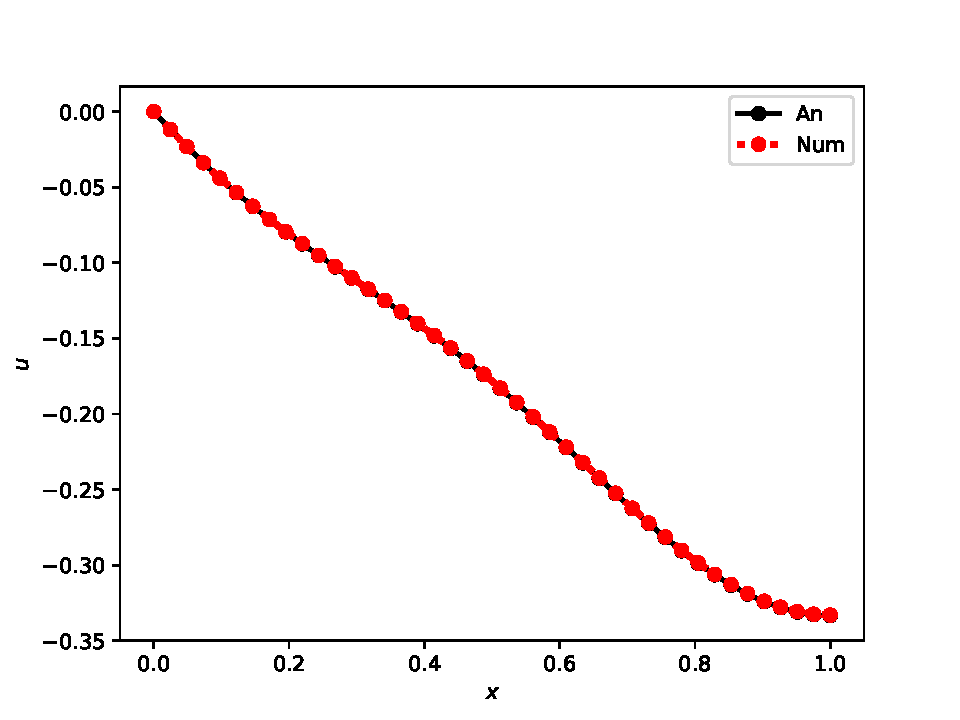
\includegraphics[width=0.85\linewidth]{plots/solutionsTask1a.pdf}\label{fig:part1Task1asolutions}}\hspace{0mm}
\subfloat[Relative error]{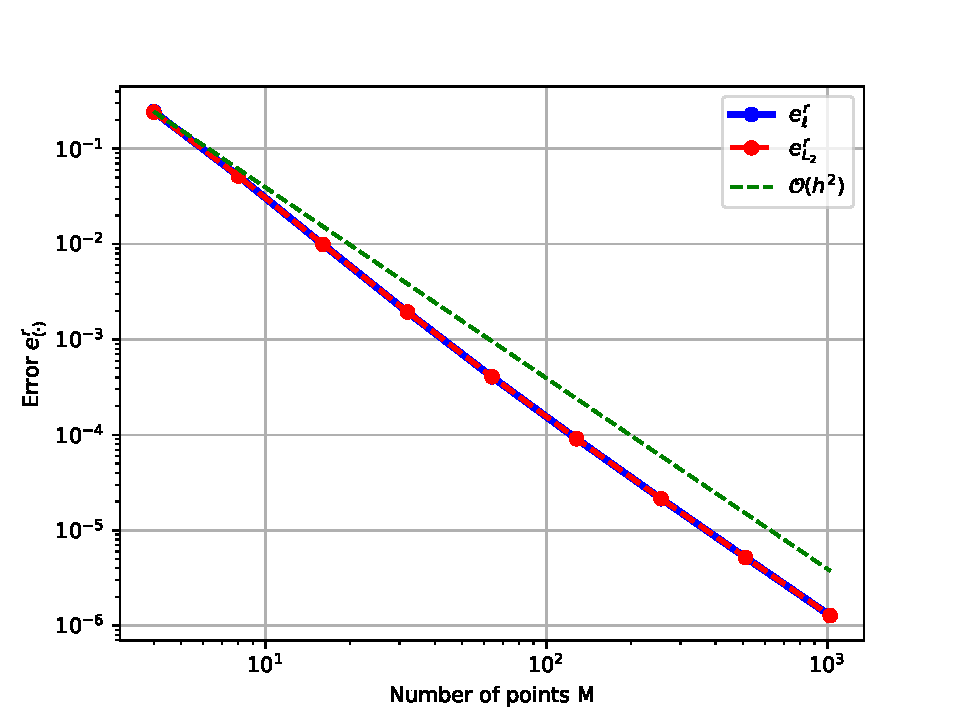
\includegraphics[width=0.85\linewidth]{plots/loglogtask1a.pdf}\label{fig:part1Task1aloglog}}\hspace{0mm}
\caption{Poisson equation with $f(x) := \cos{(2\pi x)} + x$, and boundary conditions $u(0) = 0$ and $u_x(1) = 0$. The analytical and numerical solution, solved and plotted on a grid with $M = 40$ points, is shown in (a). In (b), a "log-log" plot of relative errors when $h \rightarrow 0$ is shown.  $e^r_{L_2}$ is plotted with a dotted red line and $e^r_\ell$ is shown in blue. A green line of order $\mathcal{O}(h^2)$ is added to confirm the convergence order of the method. }
\end{figure}

In order to quantify the convergence of the numerical solution to the analytical solution, the relative errors $e_\ell^r$ and $e_{L_2}^r$, as defined in section \ref{errors.section}, are computed and plotted. 
A "$\log$-$\log$" plot of the relative errors in terms of increasing $M$ (decreasing $h \rightarrow 0$) are shown in figure \ref{fig:part1Task1aloglog}, i.e. $\log$-scales are used on both axes. The relative errors in both norms look very similar, and they show a convergence of order 2. This is, as shown, as expected. 
\newpage
\subsubsection{b)}    

A similar analysis is performed, but the boundary conditions are changed to two Dirichlet conditions

\begin{equation*}
    u(0) = 1, \, u(1) = 1.
\end{equation*}

\noindent In order to calculate the new analytical solution, a similar procedure as in part \textbf{a)} is followed. Thus, the analytical solution is given by 
\begin{equation*}
\begin{split}
    u_{xx} &= \cos{(2\pi x)} + x, \\
    u_x(x) &= \frac{1}{2\pi}\sin{(2\pi x)} + \frac12x^2 + C_1, \\
    u(x) &= -\frac{1}{4\pi^2}\cos{(2\pi x)} + \frac16x^3 + C_1x + C_2, \\
    u(0) &= -\frac{1}{4\pi^2} + C_2 = 1 \implies C_2 = 1+\frac{1}{4\pi^2}, \\
    u(1) &= -\frac{1}{4\pi^2} + \frac16 + C_1 + 1 + \frac{1}{4\pi^2} = 1 \implies C_1 = -\frac16, \\
    \implies u(x) &= -\frac{1}{4\pi^2}\cos{(2\pi x)} + \frac16x^3 -\frac16x + 1 + \frac{1}{4\pi^2}.
\end{split}
\end{equation*}
The linear system $A_h\boldsymbol{U} = \boldsymbol{f}$ is constructed, with 
\begin{equation*}
    A_h = \frac{1}{h^2}\begin{pmatrix} 
    -2 & 1 & 0 & \dots & 0 \\
    1 & -2 & 1 & \ddots & 0 \\
    \ddots & \ddots & \ddots & \ddots & \ddots \\
    0 & \ddots & 1 & -2 & 1 \\
    0 & \ddots & \ddots & 1 & -2
    \end{pmatrix}, \, 
    \boldsymbol{U} = \begin{pmatrix}
    U_1 \\
    U_2 \\
    \vdots \\
    U_M \\
    \end{pmatrix}, \, \boldsymbol{f} = \begin{pmatrix}
    f(x_1) - \frac{1}{h^2} \\
    f(x_2) \\
    \vdots \\
    f(x_M) - \frac{1}{h^2}\\
    \end{pmatrix}.
\end{equation*}
In this case, the central difference approximation \eqref{centralDiff1a)} is used for all points on the grid, except for the end points, where the function values are know. The analytical solution, as well as the numerical solution, is plotted in figure \ref{fig:part1Task1bsolutions}. Second order convergence is expected, because the central finite difference scheme has a local truncation error of order $\mathcal{O}(h^2)$. The "$\log$-$\log$" plot, shown in figure \ref{fig:part1Task1bloglog}, confirms that the convergence is of second order. 

\begin{figure}
\centering
\subfloat[Analytical and numerical solution]{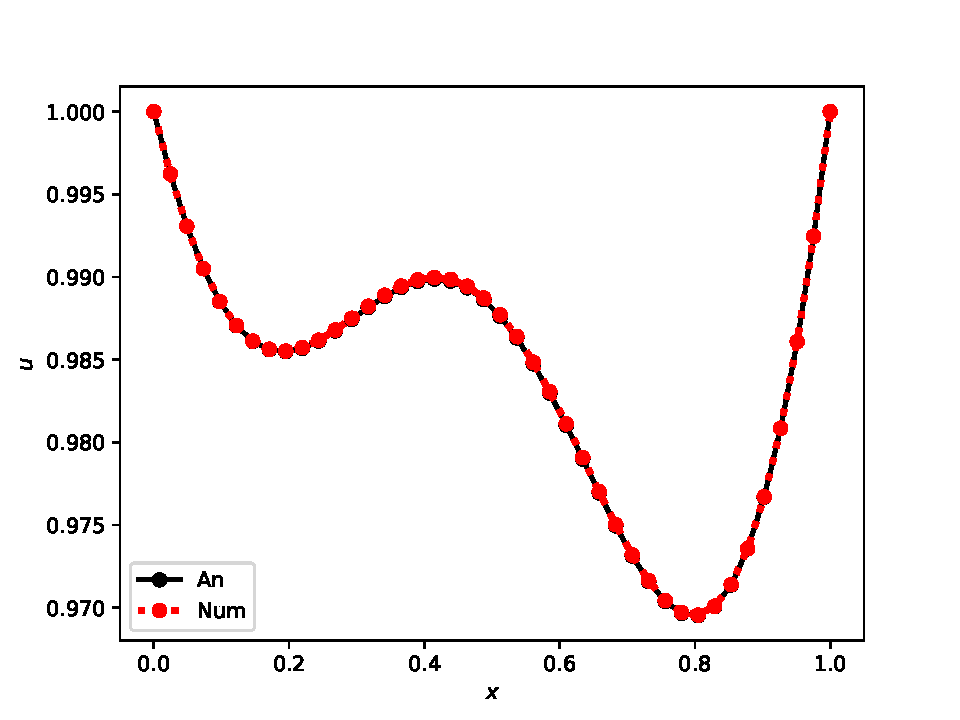
\includegraphics[width=0.85\linewidth]{plots/solutionsTask1b.pdf}\label{fig:part1Task1bsolutions}}\hspace{0mm}
\subfloat[Relative error]{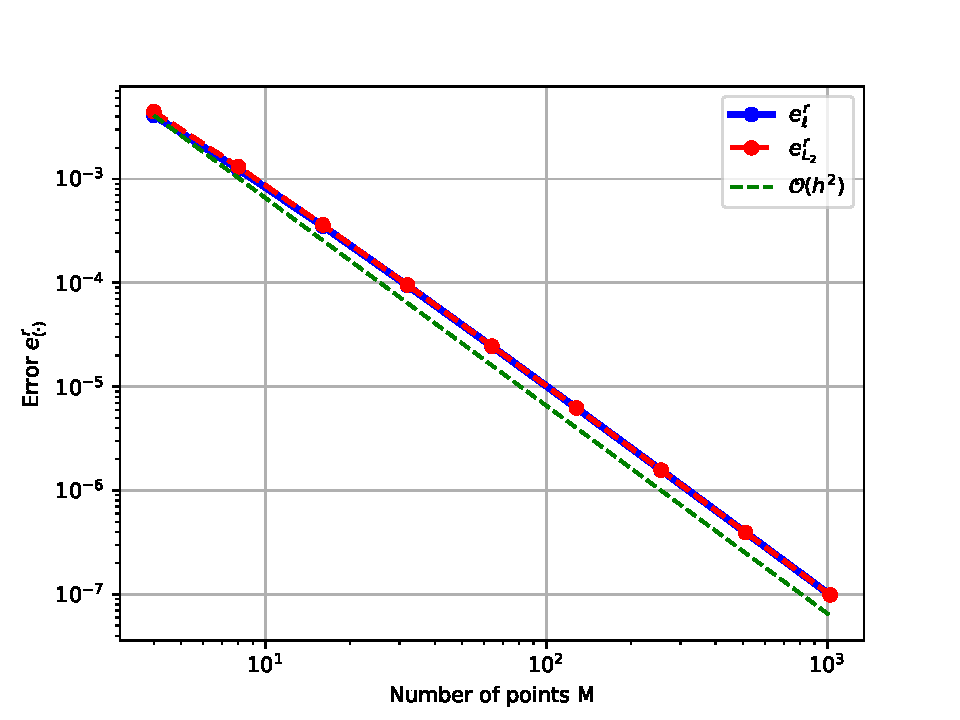
\includegraphics[width=0.85\linewidth]{plots/loglogtask1b.pdf}\label{fig:part1Task1bloglog}}\hspace{0mm}
\caption{Poisson equation with $f(x) := \cos{(2\pi x)} + x$, and boundary conditions $u(0) = 1$ and $u(1) = 1$. The analytical and numerical solution, solved and plotted on a grid with $M = 40$ points, is shown in (a). In (b), a "log-log" plot of relative errors when $h \rightarrow 0$ is shown. $e^r_{L_2}$ is plotted with a dotted red line and $e^r_\ell$ is shown in blue. A green line of order $\mathcal{O}(h^2)$ is added to confirm the convergence order of the method. }
\end{figure}

\subsubsection{c)}

The same problem is considered, but with two Neumann boundary conditions $u_x(0) = 0, \, u_x(1) = \frac{1}{2}$ instead. The issue with this specification is that the two Neumann conditions are the only conditions imposed, so the solution of the equation is ambiguous. The equation has either infinitely many solutions or zero solutions. This can be readily seen when solving the equation analytically, since there is one extra constant, $C_2$, that cannot be determined without imposing more conditions. A remedy could be to add a Dirichlet condition in at least one of the endpoints. In this way, one unambiguous solution can be determined down to the constant $C_2$. If this is done, the problem becomes very similar to the problem of task \textbf{a)}, and the numerical solution can be found in a similar manner. 

Another way to notice that the system is ambiguous is to consider a finite difference scheme with two fictitious nodes. A second order discretization of the Neumann boundary conditions using two fictitious external nodes $x_{-1}$ and $x_{M+2}$ is given by 
\begin{equation*}
    \frac{U_{1}-U_{-1}}{2h} = 0, \hspace{3mm} \frac{U_{M+2}-U_{M}}{2h} = \frac12.
\end{equation*}
These approximate boundary conditions lead to the elimination of the fictitious nodes $U_{-1} = U_1$ and $U_{M+2} = h + U_M$. Combining this with the second order central difference approximation \eqref{centralDiff1a)}, where the numerical solutions $U_m$ are inserted and the truncation error neglected, gives the equation for $m = 0$ 

\begin{comment}
    \begin{equation}
    \label{centralDifference}
        \frac{1}{h^2}(U_{m-1} - 2U_m + U_{m+1}) = f_m, \hspace{3mm} m = 0, \dots, M+1,
    \end{equation}
\end{comment}

\begin{equation*}
    \frac{U_1 - U_0}{h} = \frac{h}{2}f(x_0)
\end{equation*}
and the equation for $m = M+1$ 
\begin{equation*}
    \frac{U_M-U_{M+1}}{h} = \frac{h}{2}f(x_{M+1}) - \frac{1}{2}
\end{equation*}
Hence, the linear system takes the form

\begin{equation*}
    A_h = \frac{1}{h^2}\begin{pmatrix} 
    -h & h & 0 & \dots & 0 \\
    1 & -2 & 1 & \ddots & 0 \\
    \ddots & \ddots & \ddots & \ddots & \ddots \\
    0 & \ddots & 1 & -2 & 1 \\
    0 & \dots & \dots & h & -h
    \end{pmatrix}, \, 
    \boldsymbol{U} = \begin{pmatrix}
    U_0 \\
    U_1 \\
    \vdots \\
    U_{M+1} 
    \end{pmatrix}, \, \boldsymbol{f} = \begin{pmatrix}
    \frac{h}{2}f(x_0) \\
    f(x_1) \\
    \vdots \\
    \frac{h}{2}f(x_{M+1}) - \frac{1}{2}
    \end{pmatrix}.
\end{equation*}
It is apparent that the matrix $A_h$ is singular. Finally, the conclusion is that it cannot be solved.

\subsubsection{d)}

In this problem, the function $u(x) = \exp{\left(-\frac{1}{\epsilon}(x-\frac{1}{2})^2\right)}$ will be used as a manufactured solution for the boundary value problem 
\begin{equation}
    u_{xx} = f(x) \hspace{2mm} \text{in} \hspace{2mm} \Omega = (0,1),
\end{equation}
with Dirichlet boundary conditions $u(0) = \exp{\left(-\frac{1}{4\epsilon}\right)}$ and $u(1) = \exp{\left(-\frac{1}{4\epsilon}\right)}$. The constant $\epsilon$ determines the "steepness" of the curve, where the value $\epsilon = 0.01$ is used in our implementation. The function $f(x)$ can be calculated analytically from the manufactured solution

\begin{equation*}
\begin{split}
    f(x) &= \frac{\mathrm{d}^2}{\mathrm{d}x^2}\left(\exp{\left(-\frac{1}{\epsilon}\left(x-\frac{1}{2}\right)^2\right)}\right)\\ &= \frac{\mathrm{d}}{\mathrm{d}x}\left(-\frac{2}{\epsilon}\left(x-\frac{1}{2}\right)\exp{\left(-\frac{1}{\epsilon}\left(x-\frac{1}{2}\right)^2\right)}\right) \\
    &= -\frac{2}{\epsilon}\exp{\left(-\frac{1}{\epsilon}\left(x-\frac{1}{2}\right)^2\right)} + \frac{2}{\epsilon}\left(x-\frac{1}{2}\right)\frac{2}{\epsilon}\left(x-\frac{1}{2}\right)\exp{\left(-\frac{1}{\epsilon}\left(x-\frac{1}{2}\right)^2\right)} \\
    &= \frac{2}{\epsilon^2}\exp{\left(-\frac{1}{\epsilon}\left(x-\frac{1}{2}\right)^2\right)}\left(2\left(x-\frac{1}{2}\right)^2 -\epsilon \right).
\end{split}
\end{equation*}

How the numerical solutions converges to the manufactured solution is investigated for both second and first order methods using uniform mesh refinement (UMR) and adaptive mesh refinement (AMR).  

UMR will be used first, starting with the \textbf{first order method}. As seen from \eqref{Theory_approx_double_derivative} in section \ref{section_2.2}, applying the forward difference operator twice gives a first order approximation to the second derivative
\begin{equation*}
    \begin{split}
        &u_{xx}(x_m) = \frac{1}{h^2}\Delta^2u(x_m) + \mathcal{O}(h)\\
        \Rightarrow &f(x_m) = \frac{1}{h^2}(U_m-2U_{m+1}+U_{m+2}) \text{,} \hspace{2mm} 0 \leq m \leq M-1.
    \end{split}
\end{equation*}

\begin{comment}
\textcolor{red}{Old version;}
UMR will be used first, starting with the \textbf{first order method}. Applying the forward difference operator twice gives a first order approximation to the second derivative 
\begin{equation*}
\begin{split}
    u_{xx}(x_m) &= \frac{1}{h^2}\Delta^2u(x_m) + h\partial_x^3u(x_m) + \dots \\
    &= \frac{1}{h^2}\Delta(u(x_{m+1})-u(x_m)) + h\partial_x^3u(x_m) + \dots \\
    &= \frac{1}{h^2}(u(x_{m+2})-2u(x_{m+1}) + u(x_m)) + h\partial_x^3u(x_m) + \dots \\
    \implies
    f(x_i) &= \frac{1}{h^2}(U_i - 2U_{i+1} + U_{i+2}).
\end{split}
\end{equation*}
\textcolor{red}{Stop old version.}
\end{comment}

\noindent The implication follows from inserting the numerical approximation $U_m$ at each grid point $x_m$ and neglecting the truncation error $\mathcal{O}(h)$. 
\begin{figure}[t]
\centering
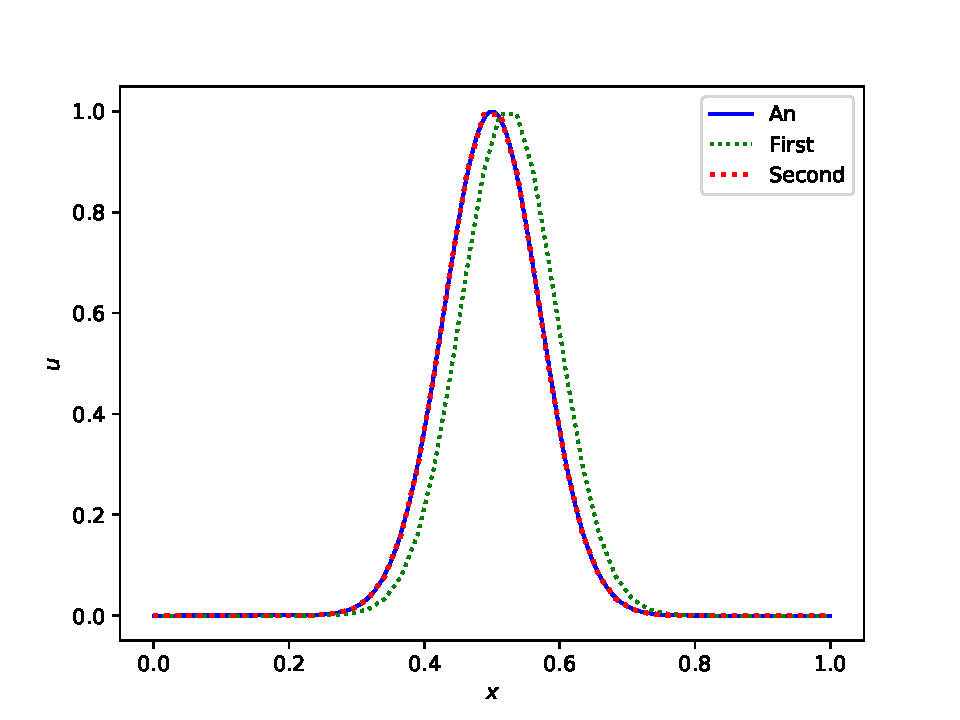
\includegraphics[width=0.85\linewidth]{plots/solutionTask1dUMR.pdf}
\caption{Poisson equation with manufactured solution $u(x) = \exp{\left(-\frac{1}{\epsilon}(x-\frac{1}{2})^2\right)}$, with Dirichlet boundary conditions $u(0) = u(1) = \exp{\left(-\frac{1}{4\epsilon}\right)}$. The manufactured solution, and numerical solutions solved with \textbf{UMR}, are plotted on a grid with $M = 40$ points. "First" refers to the solution using the first order method, while "Second" refers to the solution using the second order method.}
\label{fig:part1Task1dSolutionUMR}
\end{figure}
Adding the boundary conditions $U_0 = \alpha_1$ and $U_{M+1} = \alpha_2$ gives the linear system $A_h\boldsymbol{U} = \boldsymbol{f}$, with 

\begin{equation*}
    A_h = \frac{1}{h^2}\begin{pmatrix} 
    -2 & 1 & 0 & \dots & 0 \\
    1 & -2 & 1 & \ddots & 0 \\
    \ddots & \ddots & \ddots & \ddots & \ddots \\
    0 & \ddots & 1 & -2 & 1 \\
    0 & \dots & \dots & 1 & -2
    \end{pmatrix}, \, 
    \boldsymbol{U} = \begin{pmatrix}
    U_1 \\
    U_2 \\
    \vdots \\
    U_M 
    \end{pmatrix}, \, \boldsymbol{f} = \begin{pmatrix}
    f(x_0) - \alpha_1/h^2 \\
    f(x_1) \\
    \vdots \\
    f(x_{M-1}) - \alpha_2/h^2
    \end{pmatrix}.
\end{equation*}

The \textbf{second order method} is 

\begin{equation*}
    A_h = \frac{1}{h^2}\begin{pmatrix} 
    -2 & 1 & 0 & \dots & 0 \\
    1 & -2 & 1 & \ddots & 0 \\
    \ddots & \ddots & \ddots & \ddots & \ddots \\
    0 & \ddots & 1 & -2 & 1 \\
    0 & \dots & \dots & 1 & -2
    \end{pmatrix}, \, 
    \boldsymbol{U} = \begin{pmatrix}
    U_1 \\
    U_2 \\
    \vdots \\
    U_M 
    \end{pmatrix}, \, \boldsymbol{f} = \begin{pmatrix}
    f(x_1) - \alpha_1/h^2 \\
    f(x_2) \\
    \vdots \\
    f(x_M) - \alpha_2/h^2
    \end{pmatrix},
\end{equation*}

\noindent where a central difference scheme, as in equation \eqref{centralDiff1a)}, is used. The manufactured solution and numerical solutions when using both first and second order methods with UMR are shown in figure \ref{fig:part1Task1dSolutionUMR}. A "$\log$-$\log$" plot of the relative errors when using both first and second order methods with UMR are shown in figure \ref{fig:part1Task1dloglogUMR}. It is apparent that the convergence orders obtained in practice match the expected theoretical convergence orders for both schemes. These expectations are based on the $\mathcal{O}(h)$ truncation error of the first order method and the $\mathcal{O}(h^2)$ truncation error of the second order method.\newline


\begin{figure}
\centering
\subfloat[]{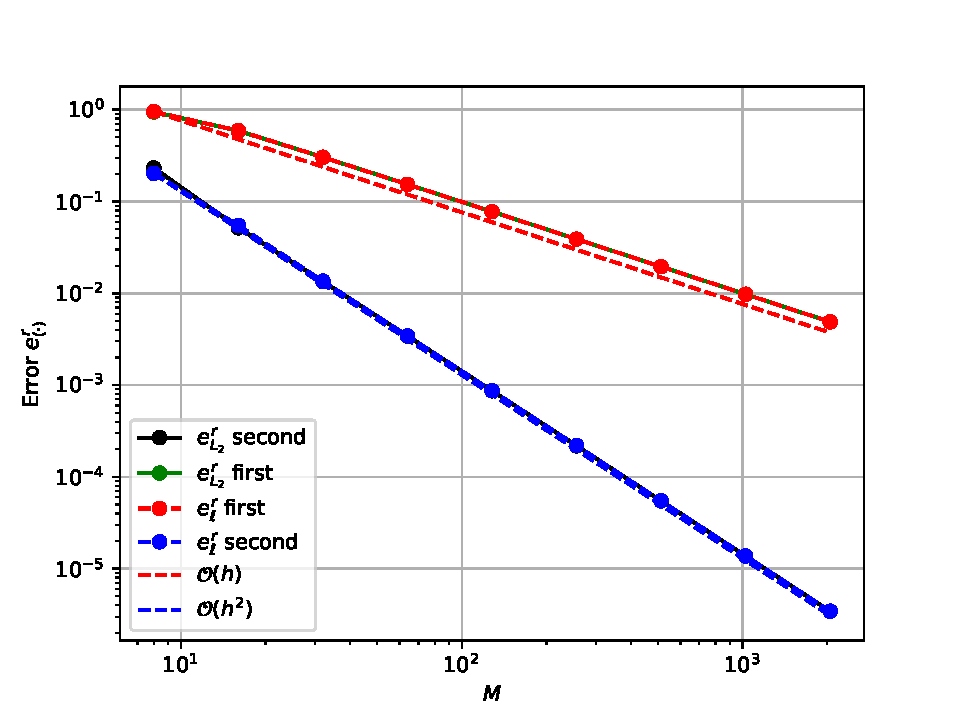
\includegraphics[width=0.85\linewidth]{plots/1d_UMR.pdf}\label{fig:part1Task1dloglogUMR}}\hspace{0mm}
\subfloat[]{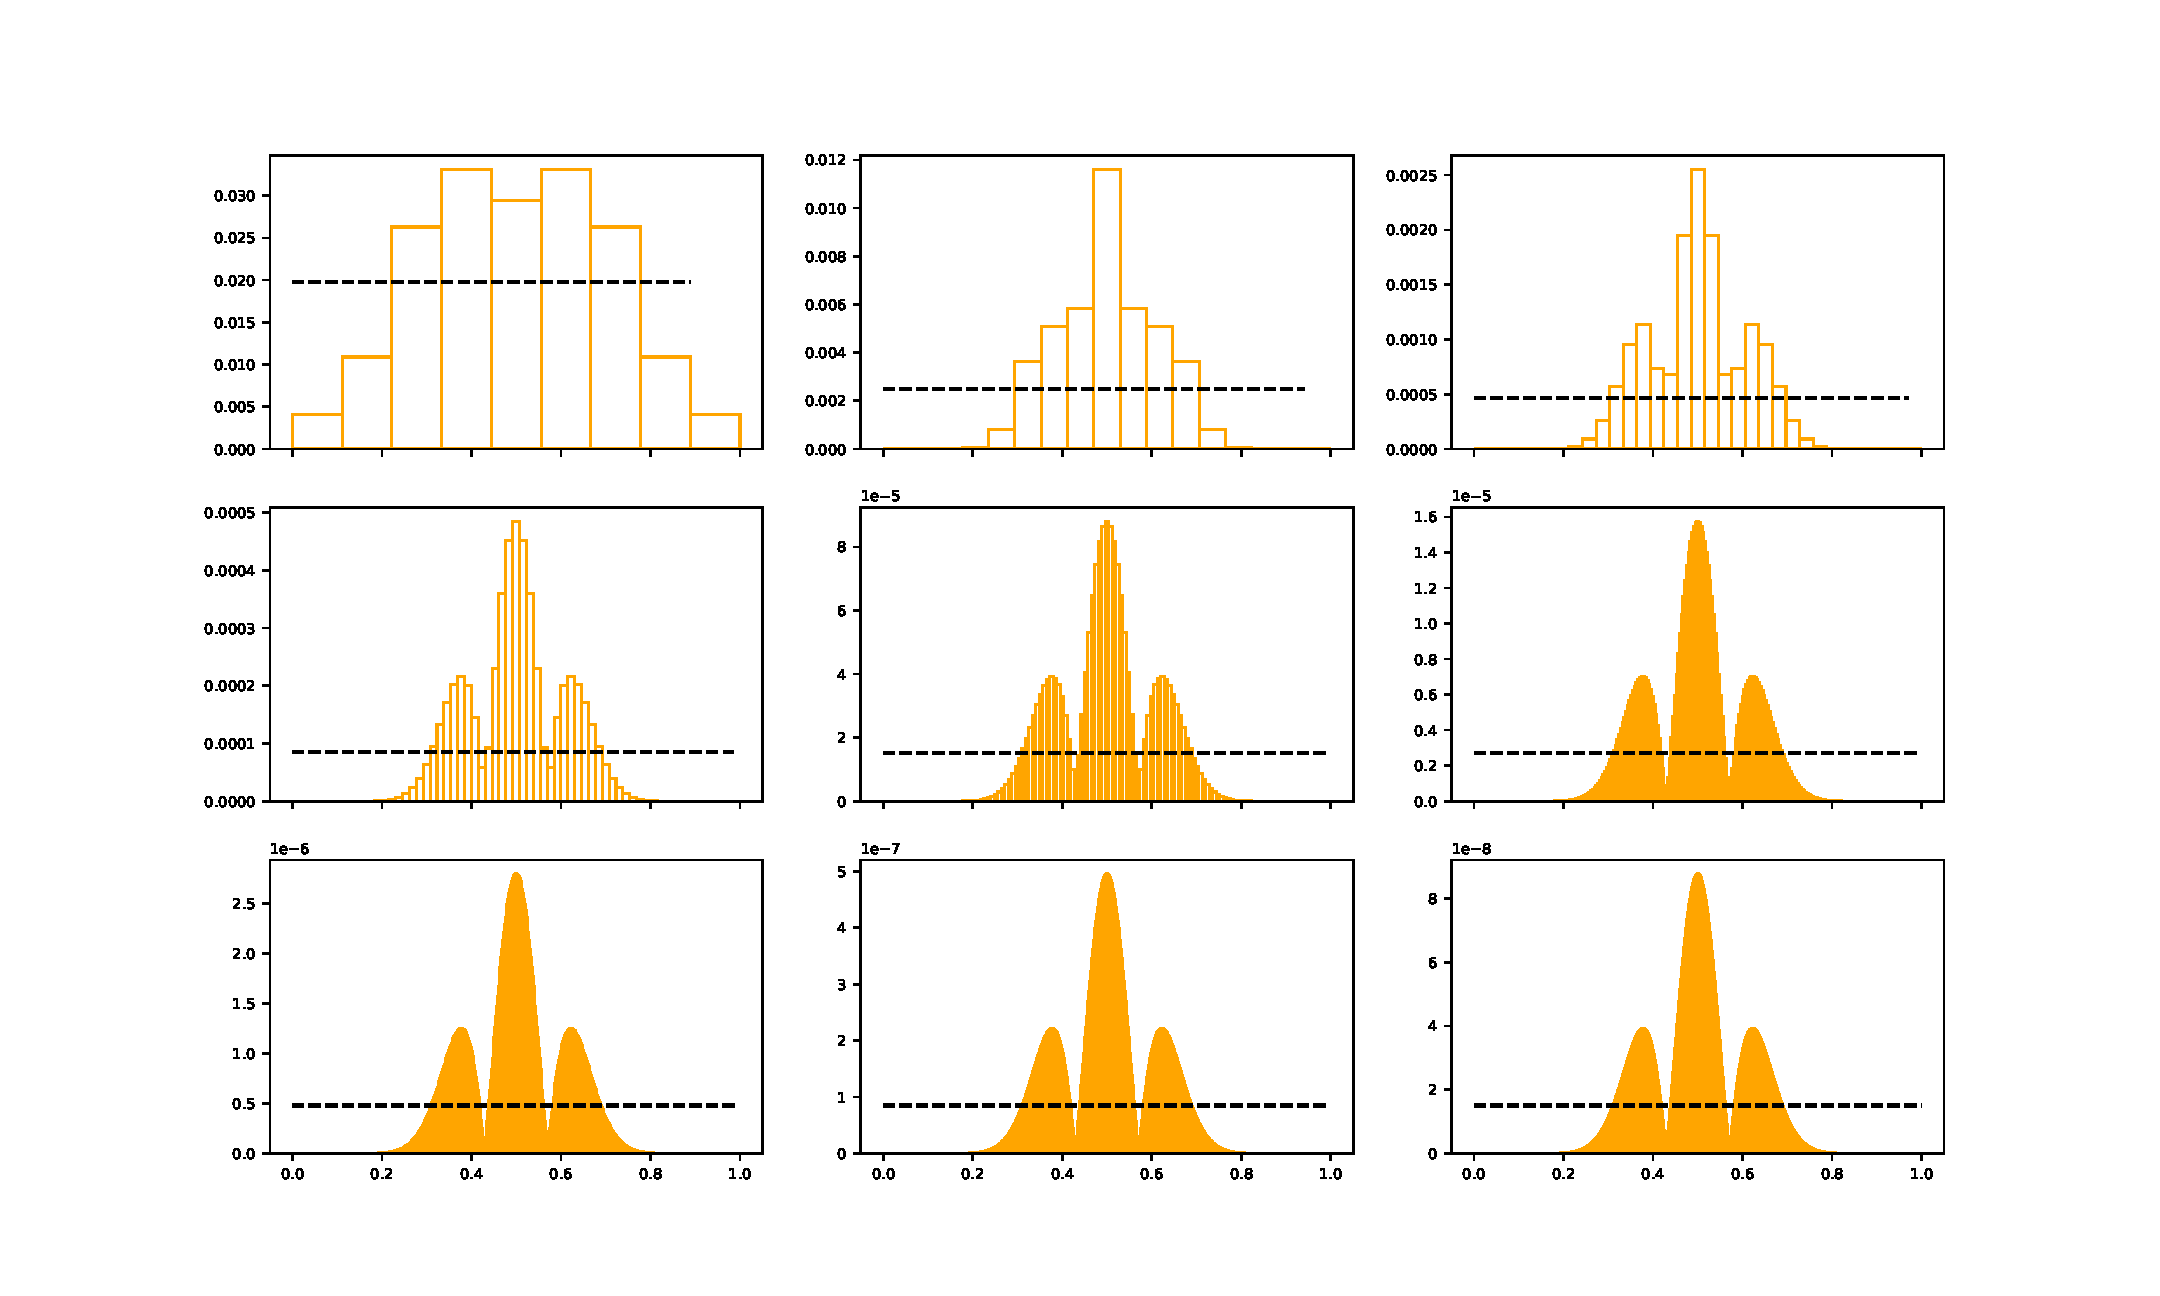
\includegraphics[width=0.85\linewidth]{plots/1d_UMR_barplot.pdf}\label{1d_UMR_barplot}}\hspace{0mm}

\caption{Poisson equation with manufactured solution $u(x) = \exp{\left(-\frac{1}{\epsilon}(x-\frac{1}{2})^2\right)}$, with Dirichlet boundary conditions $u(0) = u(1) = \exp{\left(-\frac{1}{4\epsilon}\right)}$. (a) A "log-log" plot of relative errors when $h \rightarrow 0$, when solving the problem using \textbf{UMR}, is shown. First and second order functions are added in order to compare to the convergence graphs of the numerical solutions. (b) A bar plot of the error associated with the second order solution on each sub-interval is shown. The dashed line indicates the average error. }
\end{figure}


In order to solve the boundary value problem using AMR, first and second order methods where the coefficients are dependent on the local step size need to be constructed. Liu et al. (1995) present stencils for methods of both orders in the article \textit{A high-resolution finite-difference scheme for nonuniform grids} \cite{Liu}. These are shown below. The implementation of AMR uses the average of the discrete error as the criterion for refinement. The error on each sub-interval of the grid, $I_i$ is modeled as a step-wise constant function, where the error is derived from the left end point of the interval. This means that the interval $I_i$ is split in two if

\textcolor{red}{Alt dette stemmer kanskje ikke overens med koden lenger?}
\begin{equation*}
    |u_i - U_i| \geq \frac{|u_1-U_1| + |u_2-U_2| + \dots + |u_{M-1} - U_N|}{N},
\end{equation*}
where $N$ is the number of sub-intervals at the current iteration and $u_i, U_i$ are the exact and approximate solutions at the left end-point of the $i$'th sub-interval, respectively.

A \textbf{first order method} with AMR is given by the three point stencil \cite{Liu}

\begin{equation*}
    (U_{xx})_m = bU_{m-1} - (b+c)U_{m} + cU_{m+1},
\end{equation*}
where the coefficients are given as 
\begin{equation*}
\begin{split}
    b = \frac{2}{h_{m-1}(h_{m-1}+h_{m})}, \\
    c = \frac{2}{h_{m}(h_{m-1}+h_{m})}, \\
    h_m = x_{m+1} - x_m.
\end{split}
\end{equation*}
With the Dirichlet boundary conditions, the system of equations becomes
\begin{equation*}
\begin{split}
    A_h &= \begin{pmatrix} 
    -(b+c) & c & 0 & \dots & 0 \\
    b & -(b+c) & c & \ddots & 0 \\
    \ddots & \ddots & \ddots & \ddots & \ddots \\
    0 & \ddots & b & -(b+c) & c \\
    0 & \dots & \dots & b & -(b+c)
    \end{pmatrix}, \\ 
    \boldsymbol{U} &= \begin{pmatrix}
    U_1 \\
    U_2 \\
    \vdots \\
    U_M 
    \end{pmatrix}, \, \boldsymbol{f} = \begin{pmatrix}
    f(x_1) - b\alpha_1 \\
    f(x_2) \\
    \vdots \\
    f(x_M) - c\alpha_2
    \end{pmatrix}.
\end{split}
\end{equation*}

A \textbf{second order method} with AMR is given by the four point stencil \cite{Liu}
\begin{equation}
\label{4_point_stencil}
    (U_{xx})_m = aU_{m-2} + bU_{m-1} - (a+b+c)U_m + cU_{m+1}
\end{equation}
where the coefficients are defined as
\begin{equation*}
\begin{split}
    a &= \frac{2(d_{m+1}-d_{m-1})}{d_{m-2}(d_{m-2}+d_{m+1})(d_{m-2}-d_{m-1})} \\
    b &= \frac{2(d_{m-2}-d_{m+1})}{d_{m-1}(d_{m-2}-d_{m-1})(d_{m-1}+d_{m+1})} \\
    c &= \frac{2(d_{m-2}+d_{m-1})}{d_{m+1}(d_{m-1}+d_{m+1})(d_{m-2}+d_{m+1})} \\
    d_{m+1} &=h_m, \hspace{2mm} d_{m-1} =h_{m-1}, \hspace{2mm} d_{m-2}=h_{m-2} + h_{m-1} \\ 
    h_m &= x_{m+1} - x_m.
\end{split}
\end{equation*}
By including the boundary conditions, the complete difference scheme becomes
\begin{equation*}
\begin{split}
    A_h &= \begin{pmatrix} 
    -(a+b+c) & c & 0 & \dots & \dots & 0 \\
    b & -(a+b+c) & c & \ddots & \ddots & 0 \\
    a & b & -(a+b+c) & c & \ddots & \vdots \\
    \ddots & \ddots & \ddots & \ddots & \ddots & \vdots\\
    0 & \ddots & a & b & -(a+b+c) & c \\
    0 & \dots & 0 & a & b & -(a+b+c)
    \end{pmatrix}, \, \\
    \boldsymbol{U} &= \begin{pmatrix}
    U_1 \\
    U_2 \\
    U_3 \\
    \vdots \\
    U_M 
    \end{pmatrix}, \, \hspace{2mm} \boldsymbol{f} = \begin{pmatrix}
    f(x_1) - b\alpha_1 \\
    f(x_2) - a\alpha_1\\
    f(x_3) \\
    \vdots \\
    f(x_M) - c\alpha_2
    \end{pmatrix}.
\end{split}
\end{equation*}

\begin{comment} % Vurdere hvilken som ser best ut
\begin{figure}[t]
  \centering
  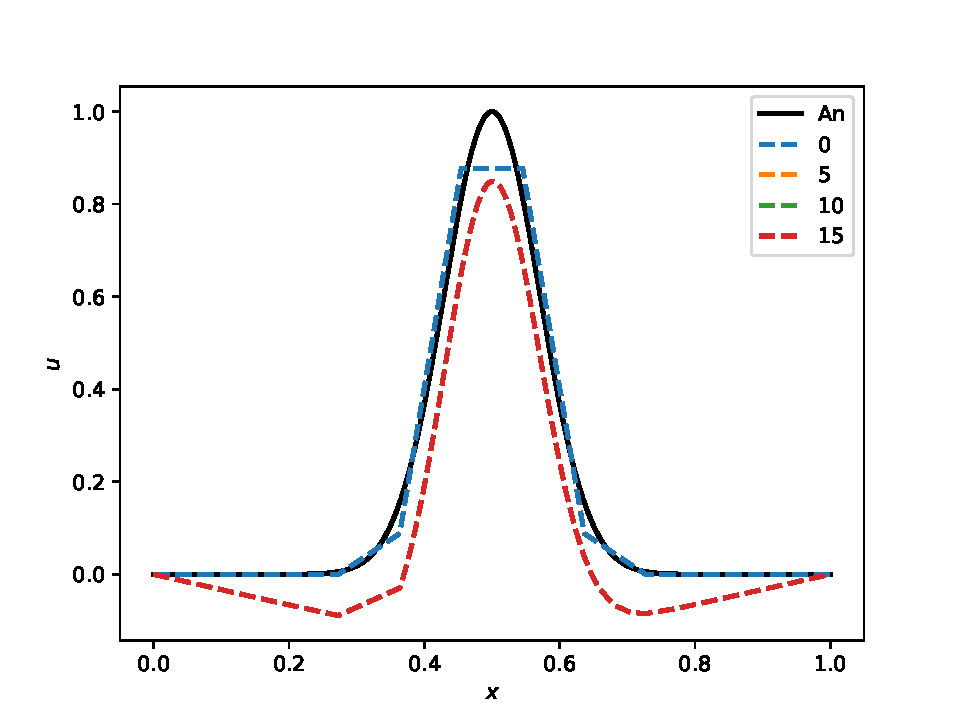
\includegraphics[width=.85\linewidth]{plots/solutionTask1dAMRFirst.pdf}
  \caption{Poisson equation with manufactured solution $u(x) = \exp{\left(-\frac{1}{\epsilon}(x-\frac{1}{2})^2\right)}$, with Dirichlet boundary conditions $u(0) = u(1) = \exp{\left(-\frac{1}{4\epsilon}\right)}$. Manufactured solution, and numerical solution solved with \textbf{AMR} and the \textbf{first order method}, plotted on a starting grid of $M = 10$ points. The grid is refined 7 times, where the integers in the legend refers to the numerical solution after each of the refinements.}

  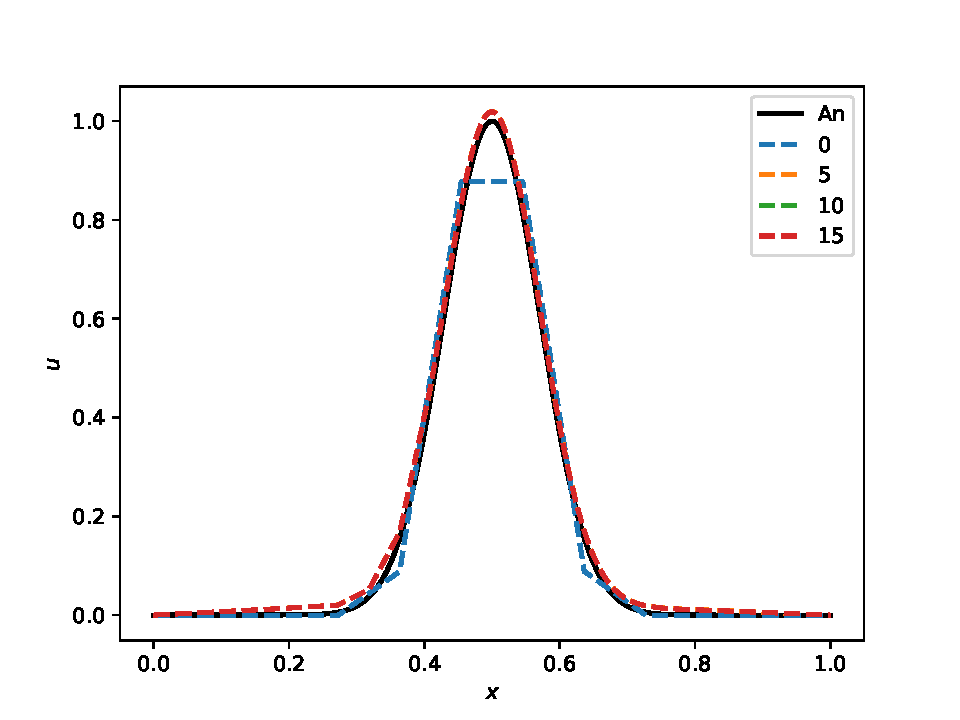
\includegraphics[width=.85\linewidth]{plots/solutionTask1dAMRSecond.pdf}
  \caption{Poisson equation with manufactured solution $u(x) = \exp{\left(-\frac{1}{\epsilon}(x-\frac{1}{2})^2\right)}$, with Dirichlet boundary conditions $u(0) = u(1) = \exp{\left(-\frac{1}{4\epsilon}\right)}$. Manufactured solution, and numerical solution solved with \textbf{AMR} and the \textbf{second order method}, plotted on a starting grid of $M = 10$ points. The grid is refined 7 times, where the integers in the legend refers to the numerical solution after each of the refinements.}
\end{figure}
\end{comment}

\begin{comment}
\begin{figure}[t]
\centering
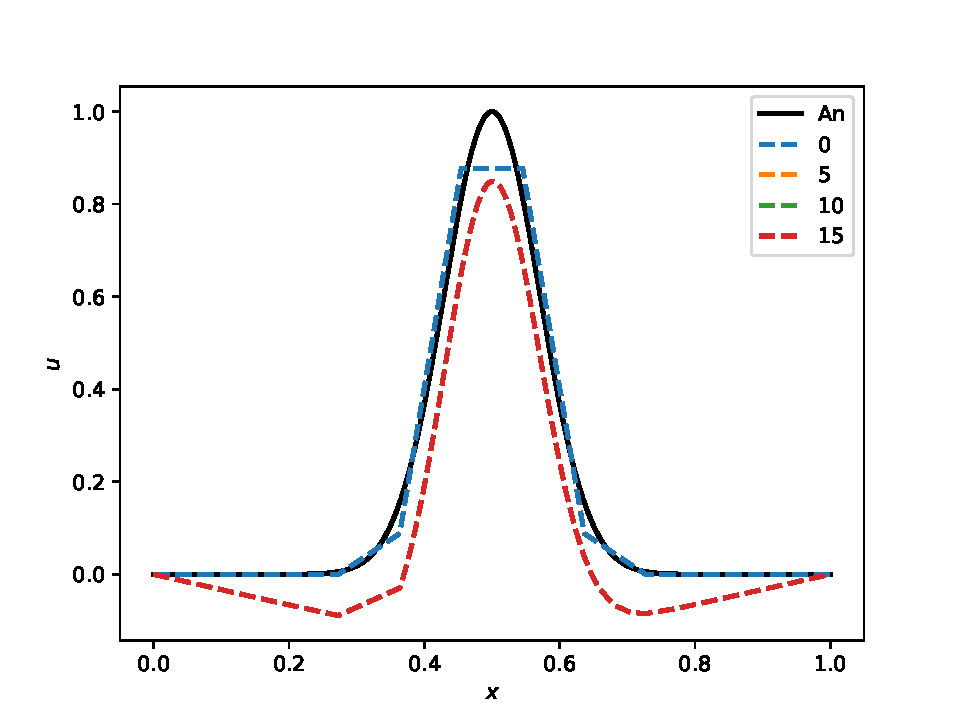
\includegraphics[width=\linewidth]{plots/solutionTask1dAMRFirst.pdf}
\caption{Poisson equation with manufactured solution $u(x) = \exp{\left(-\frac{1}{\epsilon}(x-\frac{1}{2})^2\right)}$, with Dirichlet boundary conditions $u(0) = u(1) = \exp{\left(-\frac{1}{4\epsilon}\right)}$. Manufactured solution, and numerical solution solved with \textbf{AMR} and the \textbf{first order method}, plotted on a starting grid of $M = 10$ points. The grid is refined 7 times, where the integers in the legend refers to the numerical solution after each of the refinements.}
\label{fig:part1Task1dSolutionAMRFirst}
\end{figure}

\begin{figure}[t]
\centering
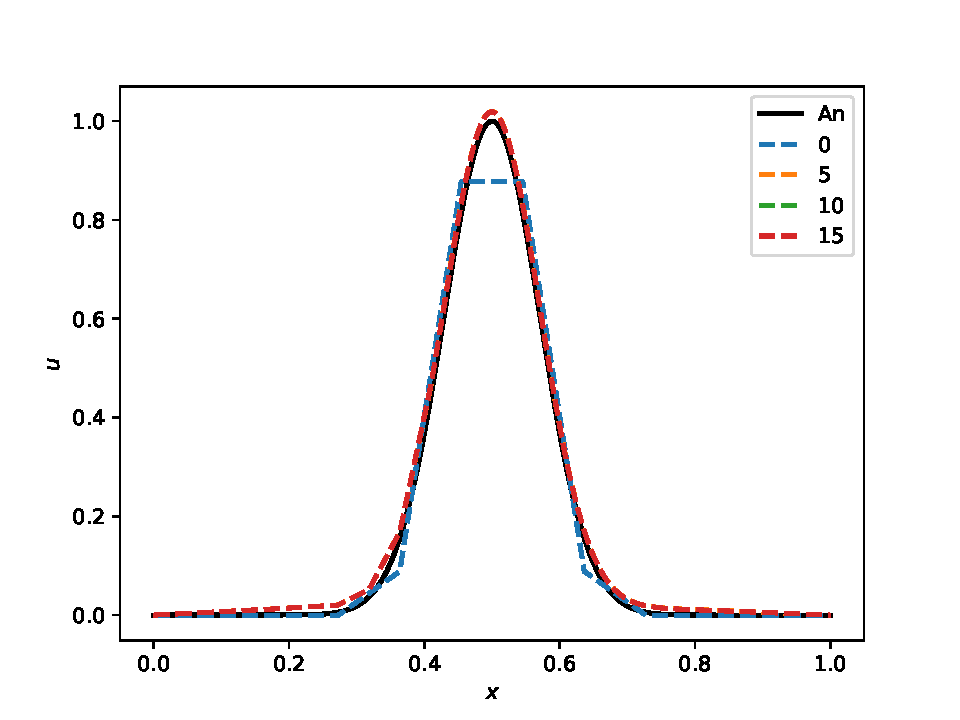
\includegraphics[width=\linewidth]{plots/solutionTask1dAMRSecond.pdf}
\caption{Poisson equation with manufactured solution $u(x) = \exp{\left(-\frac{1}{\epsilon}(x-\frac{1}{2})^2\right)}$, with Dirichlet boundary conditions $u(0) = u(1) = \exp{\left(-\frac{1}{4\epsilon}\right)}$. Manufactured solution, and numerical solution solved with \textbf{AMR} and the \textbf{second order method}, plotted on a starting grid of $M = 10$ points. The grid is refined 7 times, where the integers in the legend refers to the numerical solution after each of the refinements.}
\label{fig:part1Task1dSolutionAMRSecond}
\end{figure}
\end{comment}

We remark that for $m=1$ in equation \eqref{4_point_stencil}, the fictitious node $U_{-1}$ becomes an unknown in the linear system. To fix this, we immediately set $a_1 = 0$, by ensuring that $h_0 = h_1$ for the first two intervals. Hence, the fictitious node $U_{-1}$ is eliminated from the equation and the first equation in the linear system yields $(U_{xx})_1=\frac{1}{h_0^2}(U_0-2U_1+U_2)$. This equation also has a convergence order of $\mathcal{O}(h^2)$, because of the central difference approximation, so that the order in this AMR method is conserved.

The manufactured solution is plotted together with the numerical solutions using AMR, with both the first and second order methods, in figure \ref{fig:part1Task1dSolutionAMR}. The starting discretization of the grid in the unit interval has $M = 10$ points and the grid is possibly refined 15 times. This means that the AMR algorithm is run for 15 iterations. Whether any of the sub-intervals on the grid is refined or not during each iteration depends on whether or not the criterion is met. The numerical solution calculated after a selected set of iterations is shown. Figure \ref{fig:part1Task1dloglogAMR} shows a "log-log" plot of the discrete and continuous relative errors with AMR. It is apparent from this figure that the convergence order is more unstable with growing $M$ when using AMR compared to when using UMR. Despite this, the general trend shows that the mean convergence order follows $\mathcal{O}(h)$ for the three point stencil and $\mathcal{O}(h^2)$ for the four point stencil, which agrees with the theoretical results. \textcolor{red}{Legge til feil-plott?? :-)}

\begin{figure}
\centering
\subfloat[\textbf{AMR first order}]{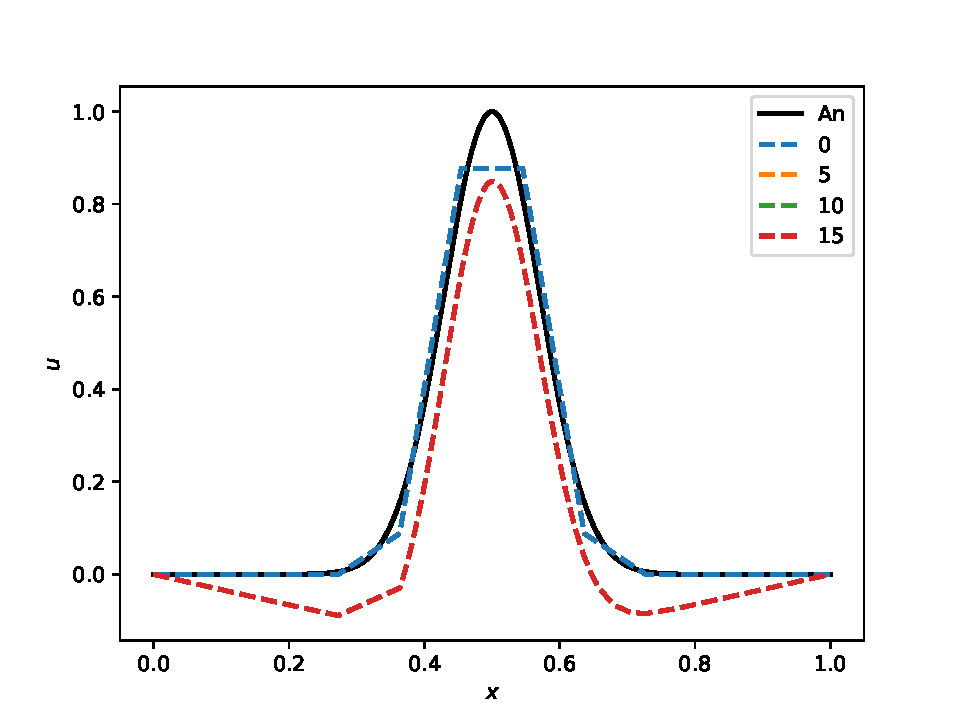
\includegraphics[width=0.85\linewidth]{plots/solutionTask1dAMRFirst.pdf}}\hspace{0mm}
\subfloat[\textbf{AMR second order}]{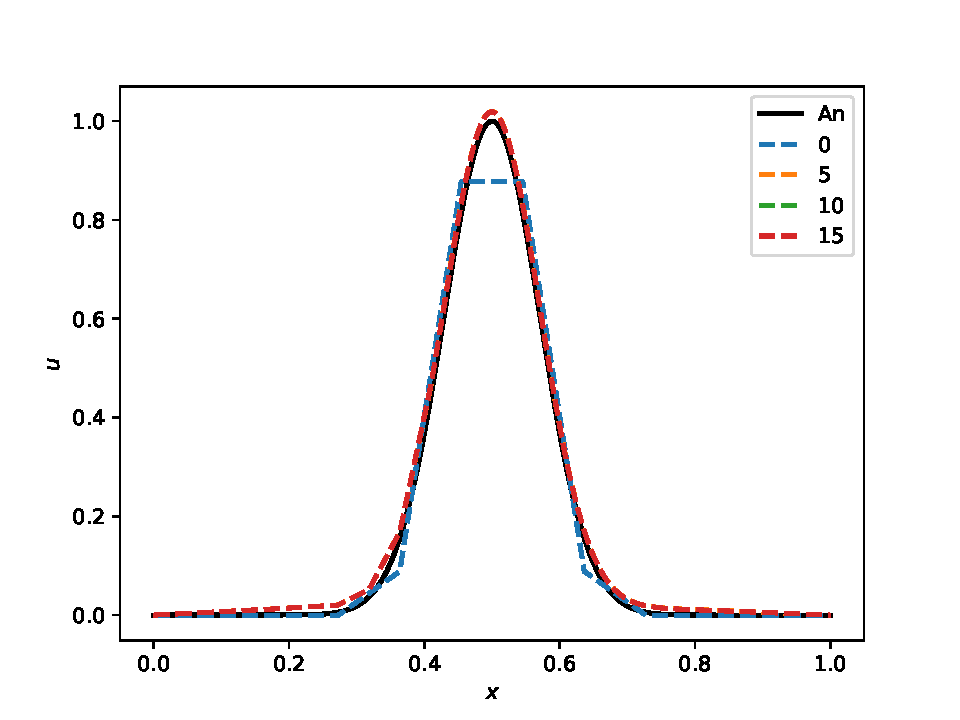
\includegraphics[width=0.85\linewidth]{plots/solutionTask1dAMRSecond.pdf}}\hspace{0mm}
\caption{Poisson equation with manufactured solution $u(x) = \exp{\left(-\frac{1}{\epsilon}(x-\frac{1}{2})^2\right)}$, with Dirichlet boundary conditions $u(0) = u(1) = \exp{\left(-\frac{1}{4\epsilon}\right)}$.  The numerical solution is computed with \textbf{AMR}, combined with a  \textbf{first order method} (a) and \textbf{second order method} (b). The integers in the legend refer to the number of iterations in the refinement, i.e. 15 refers to a solution where the grid maximally has been adaptively refined 15 times, depending on if the chosen criterion is met. The initial grid  has $M = 10$ points.}
\label{fig:part1Task1dSolutionAMR}
\end{figure}

\begin{figure}[t]
\centering
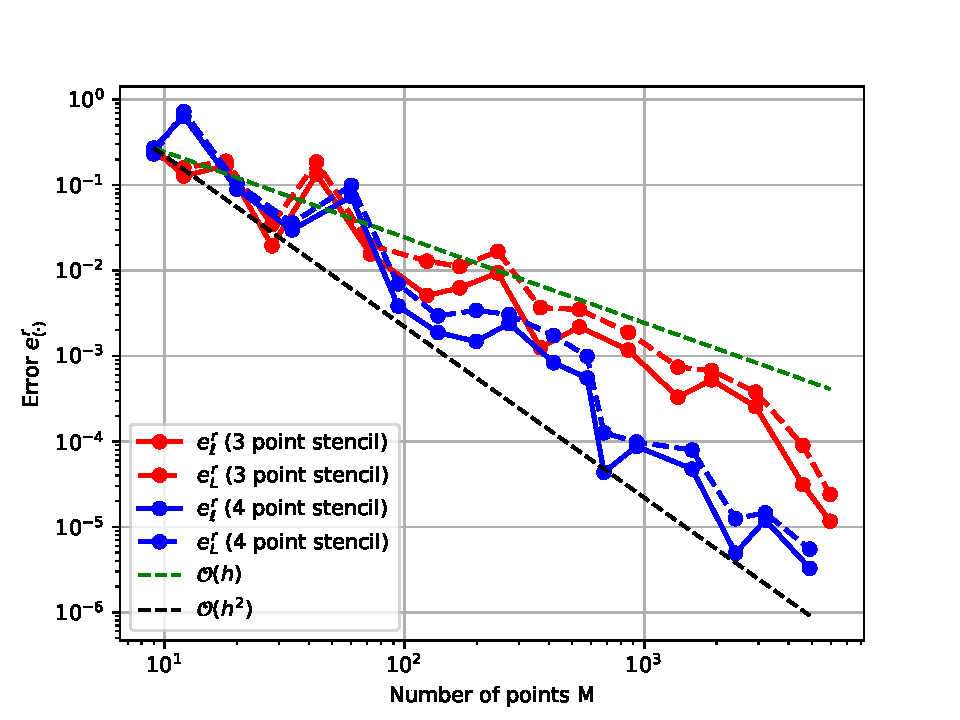
\includegraphics[width=0.85\linewidth]{plots/loglogtask1dAMR.pdf}
\caption{Poisson equation with manufactured solution $u(x) = \exp{\left(-\frac{1}{\epsilon}(x-\frac{1}{2})^2\right)}$, with Dirichlet boundary conditions $u(0) = u(1) = \exp{\left(-\frac{1}{4\epsilon}\right)}$. The graph depicts a "log-log" plot of relative errors when $h \rightarrow 0$, when solving the problem using \textbf{AMR}. First and second order functions of $h$ are added in order to compare the convergence of the numerical solution to the theoretical results.}
\label{fig:part1Task1dloglogAMR}
\end{figure}


\newpage
\ 
\newpage

\newpage

\section{Problem 2 - Heat and Inviscid Burgers' Equations}
\subsubsection{a)}
The heat equation 

\begin{equation}
    u_t = u_{xx}, \hspace{1mm} u_x(0,t) = u_x(1,t) = 0, \hspace{1mm} u(x,0) = 2\pi x - \sin{(2\pi x)},
\label{heat_eq}
\end{equation}
on $x \in [0,1], t > 0$, with Neumann boundary conditions will be studied in this problem. An equidistant grid of points in the $x$-direction

\begin{equation*}
    x_0 = 0, \, x_1 = \frac{1}{M+1}, \, \dots, \, x_M = \frac{M}{M+1}, \, x_{M+1} = 1,
\end{equation*}
will be utilized when computing the numerical solution. Semi-discretization will be used to solve the problem numerically; the PDE is discretized in the $x$-direction, before the resulting ODEs are solved with first and second order methods in time. Let $v_m(t) \approx u(x_m,t)$ for $0 \le m \le M + 1$, i.e. the numerical solution along the line $(x_m, t)$ is denoted by $v_m(t)$. For ease of notation, the explicit $t$-dependency may not be included in the following, i.e let $v_m := v_m(t)$. Furthermore, we require that 

\begin{equation}
    \dot{v}_m = \frac{1}{h^2} \delta^2 v_m = \frac{1}{h^2}(v_{m-1} - 2v_m + v_{m+1}) \quad 1 \le m \le M,
\label{cd}
\end{equation}
where $\dot{v}_m = \frac{\mathrm{d}v_m(t)}{\mathrm{d}t}$ and $h = \frac{1}{M+1}$. The boundary conditions will be discretized with both first and second order methods.
\subsubsection{First Order Discretization of Boundary Conditions}


%Discretization in the x-direction, using a forward difference scheme, gives a method of order one in x. The forward difference operator will be denoted by $\Delta u(x) = u(x+h) - u(x)$. It can be shown by Taylor expansion that $\frac{\Delta^2u(x)}{h^2}$ is an approximation of order 1 to the second derivative $u_{xx}$. This gives


%\begin{equation}
    %u_t(x_m, t) = u_{xx}(x_m, t) = \frac{1}{h^2}\Delta^2u(x_m,t) + %h\partial_x^3u(x_m,t) + \dots.
%\end{equation}

%In a similar fashion, the boundary conditions can be discretized to the first order by

%\begin{equation}
%\begin{split}
    %\partial_xu(0,t) &= 0, \\
    %\Delta u(x_0, t) &= 0 + \frac12h\partial_x^2u(x) + \dots, \\
    %\frac{u_1-u_0}{h} &= \frac12h\partial_x^2u(x) + \dots, 
%\end{split}
%\end{equation}

%and 

%\begin{equation}
%\begin{split}
    %\partial_xu(1,t) &= 0, \\
    %\Delta u(x_{M+1}, t) &= 0 + \frac12h\partial_x^2u(x) + \dots, \\
    %\frac{u_{M+2}-u_{M+1}}{h} &= \frac12h\partial_x^2u(x) + \dots, 
%\end{split}
%\end{equation}

%where we have added a fictitious node at $x_{M+2} = 1 + h$. \textcolor{red}{Usikker på om vi kunne brukt en backwards difference her i stedet, men prøver dette først i så fall. I ettertid ser det ut som at dette gjøres på side 44 i heftet, well well. Kunne jo også brukt noe annet en forward difference også, for å få en metode av orden 1.} 

%Let $v_m(t) \approx u(x_m,t)$ for $0 \le m \le M + 1$. For the method to be of order 1 and to avoid fictitious nodes, we use forward differences is the $M$ first points and backward differences in the two last points. The discretization becomes

%\begin{equation}
%\begin{split}
%\label{firstOrder}
     %&\dot{v}_m = \frac{1}{h^2}\Delta^2v(x_m,t), \quad 0\leq m \leq M-1, \\
     %&\dot{v}_m = \frac{1}{h^2}\nabla^2v(x_m,t), \quad m = M, M + 1, 
%\end{split}
%\end{equation} 


First, the left and right end points are discretized with forward and backward differences, respectively. Using the above notation, require that 

\begin{equation}
\begin{split}
     &\dot{v}_m = \frac{1}{h^2} \delta^2 v_m \quad 1 \le m \le M, \\
     &\dot{v}_0 = \frac{1}{h^2}\Delta^2v_0 \\
     &\dot{v}_{M+1} = \frac{1}{h^2}\nabla^2v_{M+1}, 
\label{diff1}
\end{split}
\end{equation} 
The boundary conditions are also discretized with forward and backward differences, which yields the following first order approximations in $h$

\begin{equation}
\begin{split}
     &-\frac{v_1-v_0}{h} = 0, \\ 
     &\frac{v_{M+1}-v_{M}}{h} = 0.
\label{bc1}
\end{split}
\end{equation} 
Combining (\ref{diff1}) and (\ref{bc1}) gives

\begin{equation}
\begin{split}
     &\dot{v}_0 = \frac{1}{h^2}(v_2 - v_0), \\
     &\dot{v}_{M+1} = \frac{1}{h^2}(v_{M-1}-v_{M+1}).
\label{bc2}
\end{split}
\end{equation} 
Finally, a linear system of ordinary differential equations can be assembled as 

\begin{equation*}
    \dot{\boldsymbol{v}} = \frac{1}{h^2}Q\boldsymbol{v},
\end{equation*}
where 

\begin{equation*}
Q = \begin{pmatrix}
    -1 & 0 & 1 & & \\
     & 1 & -2 & 1 & \\
    & & \ddots & \ddots & \ddots &\\
     & & & 1 & -2 & 1 \\
     &  & & 1& 0 & -1
    \end{pmatrix} \in \mathbb{R}^{(M+2) \times (M+2)}, \, 
    \dot{\boldsymbol{v}} = \begin{pmatrix}
    \dot{v_0} \\
    \dot{v_1} \\
    \vdots \\
    \dot{v}_{M+1} 
    \end{pmatrix} \in \mathbb{R}^{M+2}.
\end{equation*}

\subsubsection{Second Order Discretization of Boundary Conditions}

The same notation as above is adopted in this section. In order to use central differences on the boundary conditions, the fictitious nodes $x_{-1} = -h$ and $x_{M + 2} = 1 + h$ are introduced. The discretization of the boundary conditions becomes

\begin{equation}
    -\frac{v_1 -v_{-1}}{2h} = \frac{v_{M+2} - v_M}{2h} = 0.
\label{bc}
\end{equation}
Also, let

\begin{equation}
    \dot{v}_m = \frac{1}{h^2}(v_{m-1} - 2v_m + v_{m+1}) \quad 0 \le m \le M + 1.
\label{cd}
\end{equation}
Combining (\ref{bc}) with (\ref{cd}) gives $\dot{v}_0 = \frac{2}{h^2}(v_{1} - v_{0})$ and $\dot{v}_{M+1} = \frac{2}{h^2}(v_{M} - v_{M+1})$. Thus, the following system of equations

\begin{equation*}
    \dot{\boldsymbol{v}} = \frac{1}{h^2}Q\boldsymbol{v},
\end{equation*}
where 
\begin{equation*}
Q = \begin{pmatrix}
    -2 & 2 & & & \\
    1 & -2 & 1 & & \\
    & \ddots & \ddots & \ddots &\\
     & & 1 & -2 & 1 \\
     &  & & 2 & -2
    \end{pmatrix}, 
\end{equation*}
is constructed.

\subsubsection{Solution of the System of ODEs}
After a discretization of the boundary conditions is chosen and the system of ODEs

\begin{equation*}
    \dot{\boldsymbol{v}} = \frac{1}{h^2}Q\boldsymbol{v},
\end{equation*}
is assembled, a procedure for calculating the evolution of $\boldsymbol{v}$ in time needs to be chosen. This can be done with the trapezoidal rule, which amounts to the Crank-Nicolson method (hereafter denoted by CN). The Backward Euler method (hereafter denoted by BE) can also be used. Letting  $\boldsymbol{V}^0 = (u(x_0,0), \dots, u(x_{M+1},0))^T$, CN may be written as

\begin{equation*}
    \boldsymbol{V}^{n+1} = \boldsymbol{V}^n + \frac{k}{2}\left(\frac{1}{h^2}Q\boldsymbol{V}^n + \frac{1}{h^2}Q\boldsymbol{V}^{n+1} \right), 
\end{equation*}

\noindent where $k=\frac{T}{N}$ is the step length in time and $n$ denotes the current iteration. The system of equations is solved iteratively from $n=0$ to $n=N-1$ until the solution at $t_N=T$ is found. Equivalently, the method can be written as

\begin{equation}
    (I - \frac{k}{h^2}Q)\boldsymbol{V}^{n+1} = (I + \frac{k}{h^2}Q)\boldsymbol{V}^n \quad (\text{Crank-Nicolson}).
    \label{CN}
\end{equation}
Moreover, BE can be written as

\begin{equation}
    (I - \frac{k}{h^2}Q)\boldsymbol{V}^{n+1} = \boldsymbol{V}^n \quad (\text{Backward Euler}).
    \label{BE}
\end{equation}

 \noindent The local truncation error of CN and BE with second order discretization of boundary conditions are

\begin{equation}
    \begin{split}
        \tau_{CN} &= \mathcal{O}(k^2 + h^2), \\
        \tau_{BE} &= \mathcal{O}(k + h^2),
    \end{split}
\label{orders}
\end{equation}
respectively. These truncation errors can be shown using Taylor expansions around $(x_m, t_n)$. Inserting the exact solutions $\boldsymbol{U}^n = (u(x_0,t_n), \dots, u(x_{M+1},t_n))^T$ into BE gives the truncation error

\begin{equation*}
    k\tau_{BE} = (I - \frac{k}{h^2}Q)\boldsymbol{U}^{n+1} - \boldsymbol{U}^n.
\end{equation*}

\noindent Considering the system before boundary conditions are implemented, it can be written row-wise as 

\begin{equation*}
\begin{split}
    k\tau_{BE} &= (1 - \frac{k}{h^2}\delta_x^2)u_m^{n+1} - u_m^n, \quad 0 \leq m \leq M + 1\\
    &= \left(1 - k(\partial_x^2 + \mathcal{O}(h^2))(1 + k\partial_t + \frac{1}{2}k^2\partial_t^2 + \mathcal{O}(k^3))\right)u_m^n - u_m^n \\
    &= \left(k\partial_t + \frac{1}{2}k^2\partial_t^2 - k(\partial_x^2 + \mathcal{O}(h^2)) - k^2(\partial_x^2 + \mathcal{O}(h^2))\partial_t + \mathcal{O}(k^3)\right)u_m^n \\
    &= \left(-\frac{1}{2}k^2\partial_t^2 + \mathcal{O}(kh^2)\right)u_m^n \\
    &= \mathcal{O}(k^2 + kh^2), 
\end{split}
\end{equation*}
which shows that $\tau_{BE} = \mathcal{O}(k + h^2)$. A similar proof can be applied to show the order of the local truncation of CN \cite{Owren}. 

The numerical solution using CN (with second order discretization of boundary conditions) is plotted in figure \ref{2a_sol}.

\begin{figure}
\centering
\subfloat[Numerical Solution]{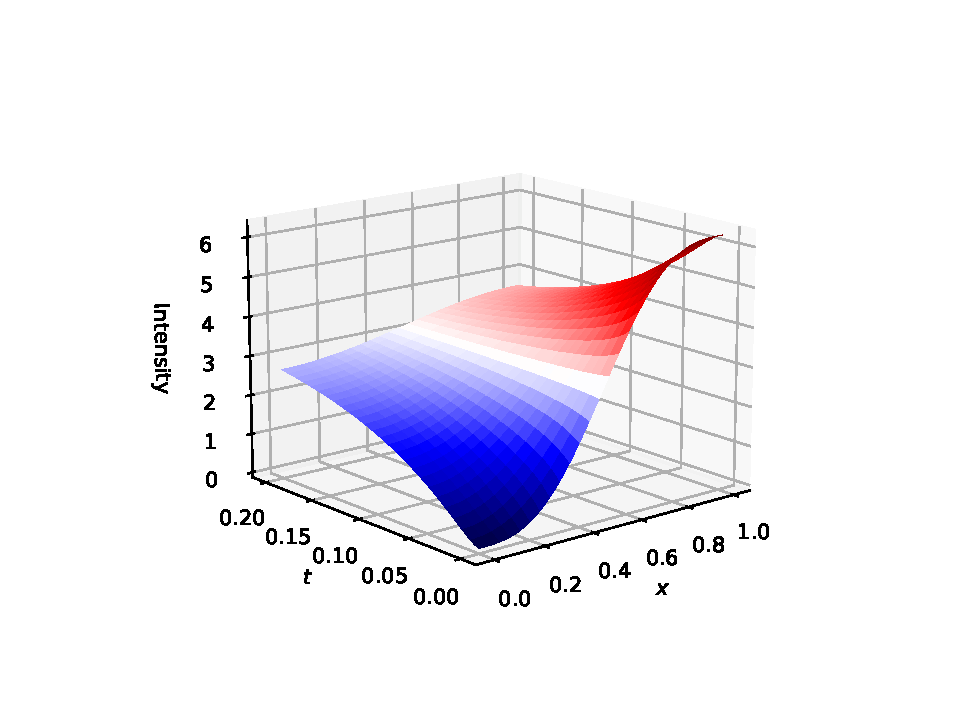
\includegraphics[width=0.9\linewidth]{plots/2a_sol.pdf}\label{2a_sol}}\hspace{0mm}
\subfloat[Relative error with $h$-refinement, 1st and 2nd order discretization of BC's]{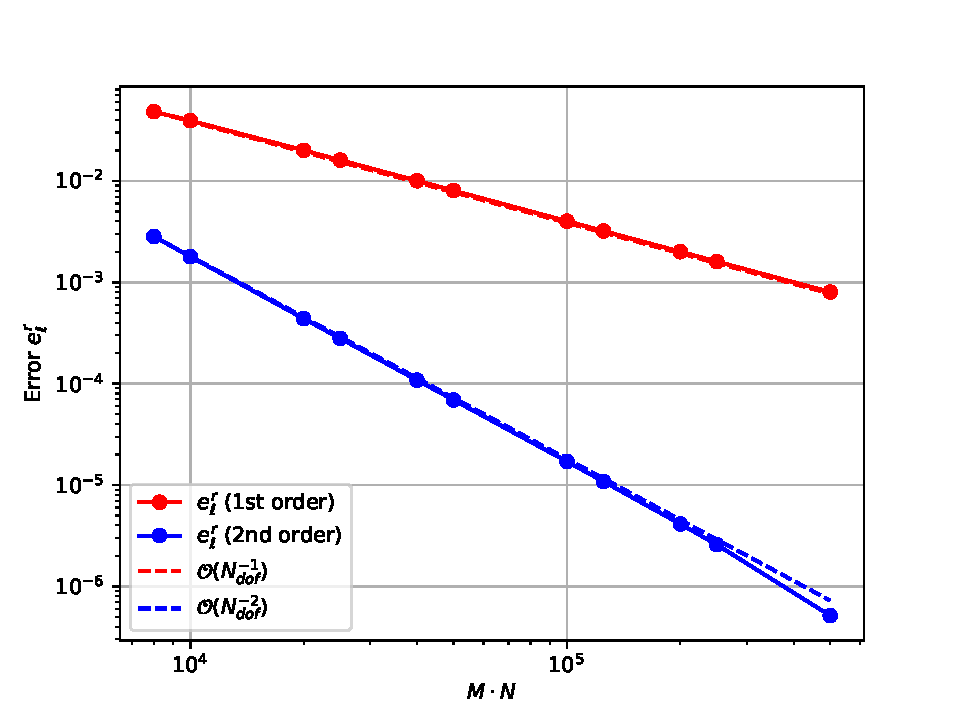
\includegraphics[width=0.85\linewidth]{plots/2a_comp.pdf}\label{2a_comp}}\hspace{0mm}
\caption{Heat equation with two Neumann boundary conditions and initial condition $u(x,0) = 2\pi x - \sin{(2\pi x)}$ on $x \in [0,1]$ and $t \in [0,0.2]$. The numerical solution, calculated using CN with $M=N=50$ and a second order discretization of the boundary conditions, is plotted in (a). The relative error with $h$-refinement for first and second order discretizations of the boundary conditions, is plotted in (b). CN was used also here with $N=1000$. The $x$-axis shows the number of degrees of freedom in the linear system.}
\end{figure}

\begin{comment}
\begin{figure}[t]
    \centering
    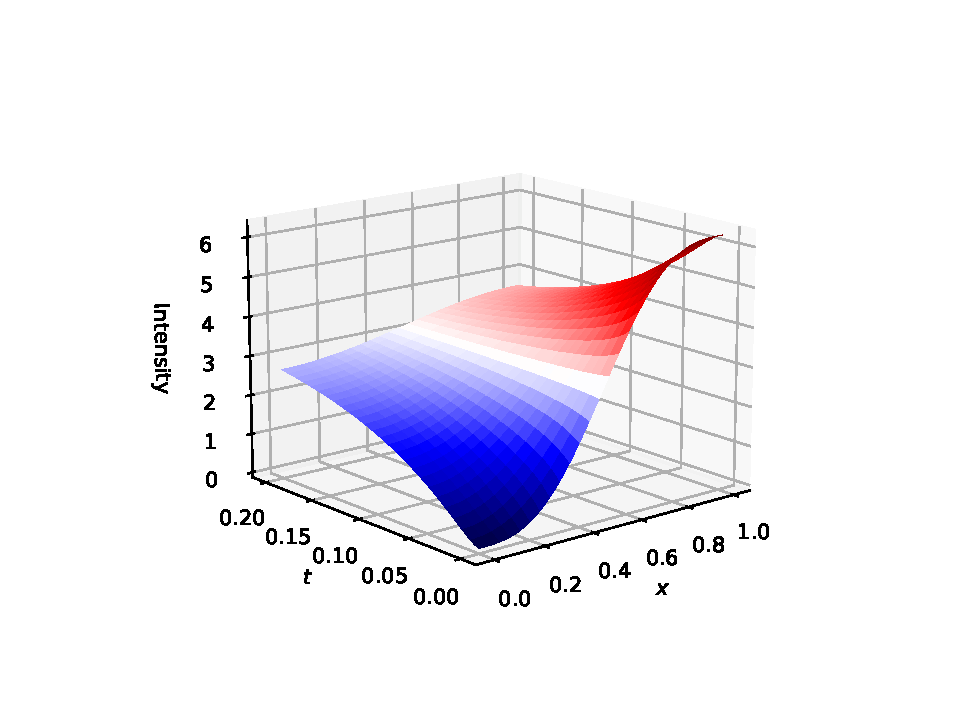
\includegraphics[width = \linewidth]{plots/2a_sol.pdf}
    \caption{Heat equation with two Neumann boundary conditions and initial condition $u(x,0) = 2\pi x - \sin{(2\pi x)}$. The numerical solution is plotted, where second order discretizations of the boundary conditions and CN is used to calculate it.}
    \label{2a_sol}
\end{figure}

\begin{figure}[t]
    \centering
    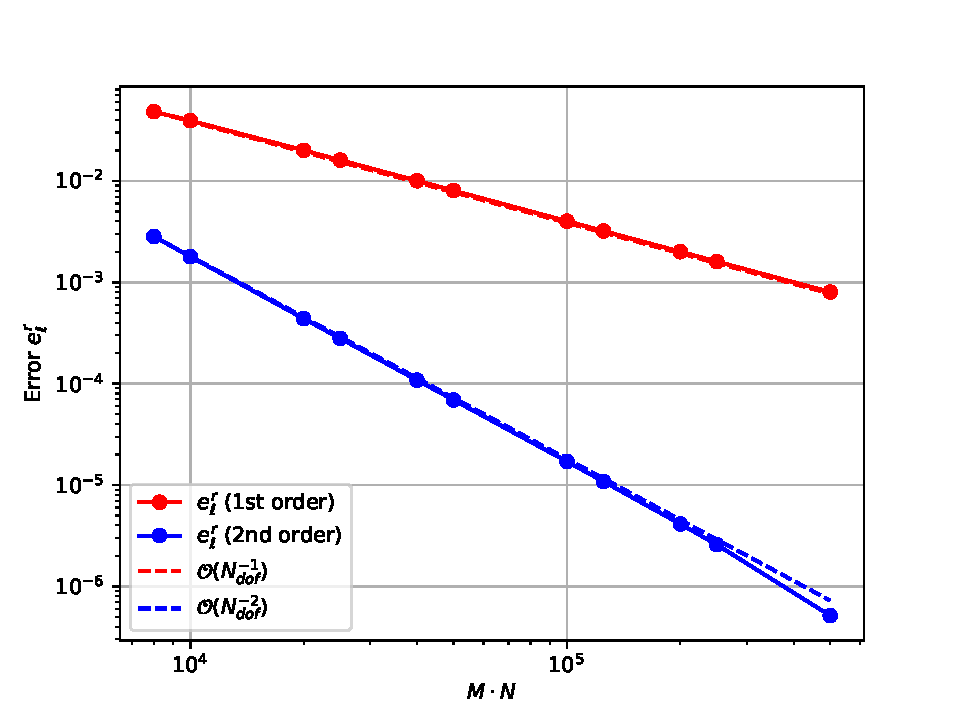
\includegraphics[width = 0.85\linewidth]{plots/2a_comp.pdf}
    \caption{Heat equation with two Neumann boundary conditions and one Dirichlet initial condition. The relative error with $h$-refinement for first and second order discretization of boundary conditions.  \textcolor{red}{Legg gjerne inn $\ell$ og $\mathcal{O}$ i figuren. Jeg har også brukt $\cdot$ på x-aksen ser jeg.}}
    \label{2a_comp}
\end{figure}
\end{comment}


\subsubsection{Convergence Plots}
For this problem, the analytical solution is not available in a closed form. Thus, in order to make convergence plots, a \textit{reference solution}, $\boldsymbol{u}_{M^*}(t)$, must be constructed. It is called a reference solution, since it is a numerical solution with a large number of points $M = M^*$ (small $h = h^*$) in the $x$-direction. Hence, it should be more precise than numerical solutions computed on grids with lower resolutions, which is why it is used as a replacement for the analytical solution when making convergence plots. Throughout this problem, this reference solution has been calculated using $M^* = 1000$ with second order discretizations of the boundary conditions, in combination with CN.

\begin{figure}
\centering
\subfloat[$h$-refinement]{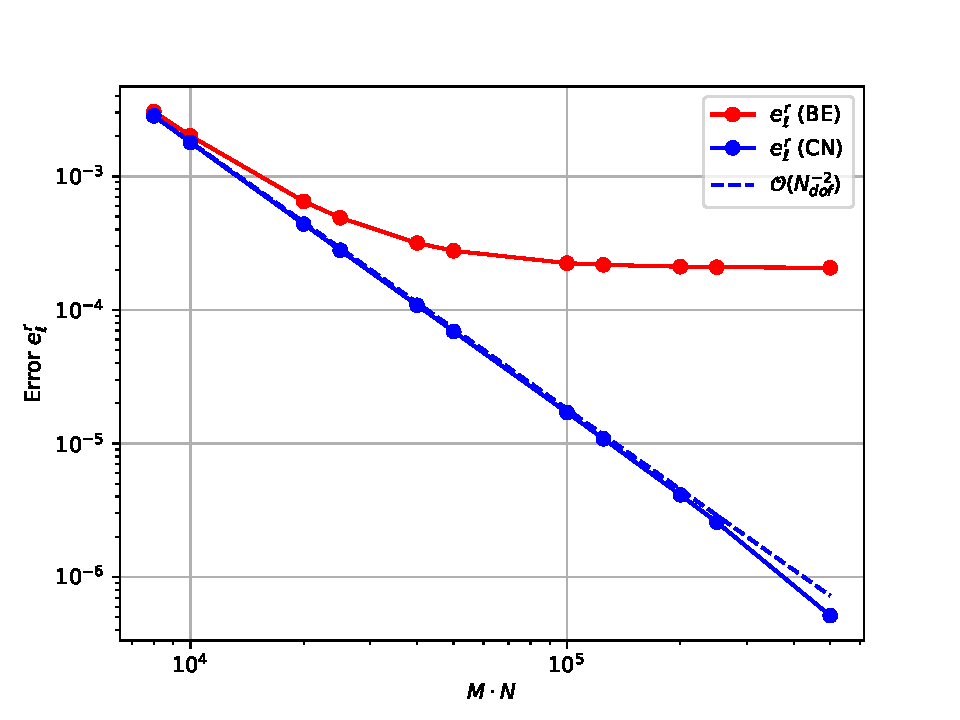
\includegraphics[width=0.85\linewidth]{plots/2a_href.pdf}\label{2a_href}}\hspace{0mm}
\subfloat[$k$-refinement]{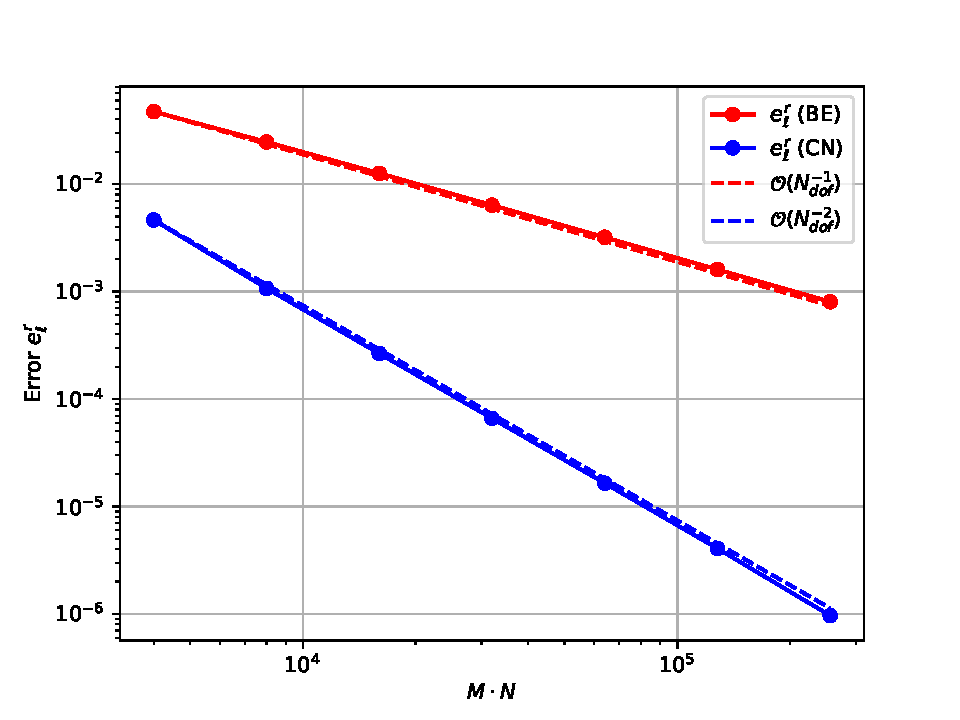
\includegraphics[width=0.85\linewidth]{plots/2a_kref.pdf}\label{2a_kref}}\hspace{0mm}
\caption{Heat equation with two Neumann boundary conditions and initial condition $u(x,0) = 2\pi x - \sin{(2\pi x)}$ on $x \in [0,1]$ and $t \in [0,0.2]$. The relative error obtained with $h$-refinement, with $N=1000$, is plotted in (a). Similarly, the relative error obtained with $k$-refinement, with $M=1000$, is plotted in (b). A second order discretization of the boundary conditions is used when calculating the numerical solution with both BE and CN. The $x$-axis shows the number of degrees of freedom in the linear system.}
\label{fig:2a_hrefAndKref}
\end{figure}

First, how the order of the boundary condition discretization impacts the convergence order with $h$-refinement, is investigated. CN is used, in order to minimize the error in time. The relative error $e_{\ell}^r$, as defined in equation \eqref{discreteRelativeError}, is calculated when increasing the resolution in the $x$-direction. Remember that the analytical solution is replaced by the reference solution in the relative error. The result is depicted in figure \ref{2a_comp}. It is apparent that a first order discretization of the boundary conditions results in first order convergence, even though the finite difference scheme used on the remaining grid points is of second order. Hence, use of the first order discretization of the boundary conditions will be avoided in the following. 

Next, $h$-refinement is considered with both BE and CN. The relative errors are computed and plotted in figure \ref{2a_href}. It is apparent that CN yields second order convergence, while the relative error for BE stagnates at a certain level. This is because BE is less accurate in time; the truncation error for BE is of order one, while for CN it is of order two, as seen in equation \eqref{orders}. In other words, the error in time is dominating the error in BN, which yields no decrease in the relative error when further increasing the spatial resolution. The point of stagnation of the decrease in the relative error for BE could be postponed to a larger number of degrees of freedom and a smaller error by, e.g., increasing the number of time steps $N$.

Furthermore, $k$-refinement, i.e. refinement along the $t$-axis, is considered. The relative errors are computed and plotted in figure \ref{2a_kref}. Note that CN yields second order convergence, while BE yields first order convergence. This is as expected from equation \eqref{orders}, because, in theory, $M$ is set to a large number ($M = 1000$ in the figure), such that the error in $x$ can be neglected, i.e. $\mathcal{O}(k^2 + h^2) = \mathcal{O}(k^2)$ and $\mathcal{O}(k + h^2) = \mathcal{O}(k)$ for CN and BE respectively. 

Finally, $h \propto k$-refinement is considered, This means that the step lengths are proportional, while they are increased at the same rate. The relative errors are calculated and the resulting convergence plot is depicted in figure \ref{rref_2a}. Note that CN yields convergence of first order, while BE yields convergence of order $\frac{1}{2}$. This is in accordance with the expected theoretical convergence orders, which are

\begin{equation*}
    \tau_{CN} = \mathcal{O}(k^2 + h^2) \overset{k \propto h} = \mathcal{O}(kh) = \mathcal{O}\left(\frac{1}{MN}\right) = \mathcal{O}(N_{\mathrm{dof}}^{-1}),
\end{equation*}
and 

\begin{equation*}
    \tau_{BE} = \mathcal{O}(k + h^2) \overset{k \propto h} = \mathcal{O}(h) = \mathcal{O}\left(\frac{1}{M}\right) = \mathcal{O}(N_{\mathrm{dof}}^{-1/2}).
\end{equation*}

\begin{figure}[t]
    \centering
    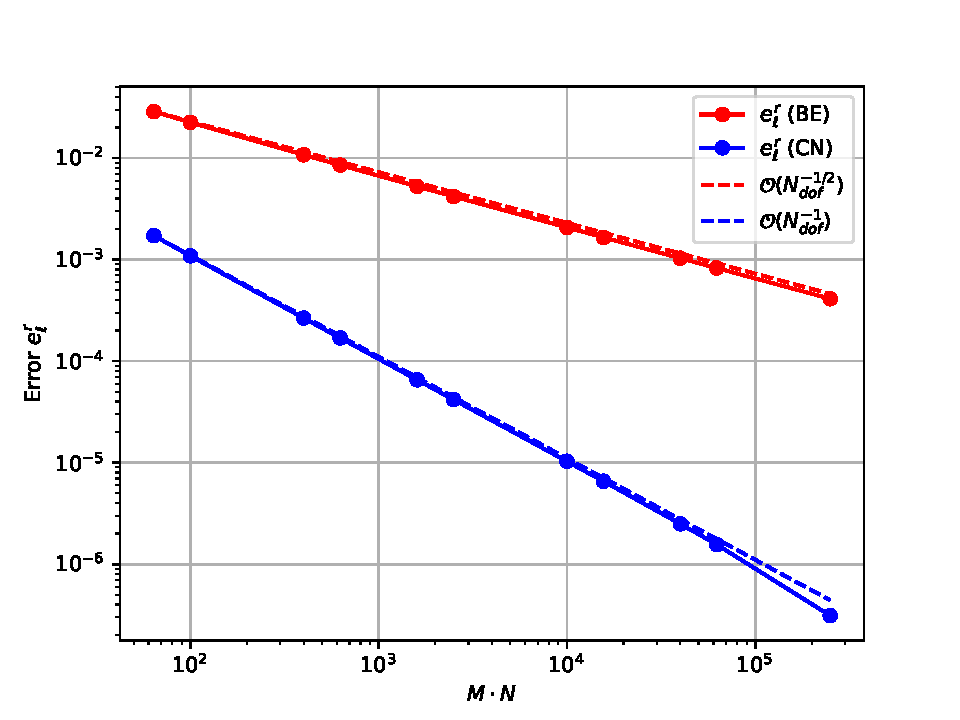
\includegraphics[width = 0.85\linewidth]{plots/rref_BEvsCN1.pdf}
    \caption{Heat equation with two Neumann boundary conditions and initial condition $u(x,0) = 2\pi x - \sin{(2\pi x)}$ on $x \in [0,1]$ and $t \in [0,0.2]$. The relative error obtained with $h \propto k$-refinement, is plotted. CN and a second order discretization of the boundary conditions is used when calculating the numerical solution. The $x$-axis shows the number of degrees of freedom in the linear system.}
    \label{rref_2a}
\end{figure}


\newpage
\subsubsection{b)}
In this subsection, the heat equation 
\begin{equation}
\begin{split}
    &u_t = u_{xx} \hspace{2mm} \text{in} \hspace{2mm} \Omega(x,t): x \in [0,1], t \in [0,T], \\ &u(0,t)=u(1,t)=0,
\label{2b}
\end{split}
\end{equation}
will be solved. $T = 0.2$ is used in the following. By Fourier analysis, a general solution is on the form \cite{Kreyszig}
\begin{equation*}
    u(x,t) = \sum_{n=1}^{\infty} D_n e^{-\pi^2 n^2 t} \sin{(n \pi x)}.
\end{equation*}
Given an initial value $u(x,0)=f(x)$, the coefficients $D_n$ can be determined using the sine orthogonality

\begin{equation*}
    D_n = 2 \int_{0}^{1} f(x) \sin{(n \pi x)} \mathrm{d}x.
\end{equation*}
Now, for simplicity, the initial value $f(x)=3\sin{(2 \pi x)}$ is chosen, which yields a simple manufactured solution on the form 

\begin{equation}
\label{2b-analytical-solution}
    u(x,t) = 3 e^{-4 \pi^2 t} \sin{(2 \pi x)}, 
\end{equation}
since $D_n = 0, \hspace{1mm} \forall n \in \{1\} \cup [3, \infty)$, and $D_2 = \frac12$.
The numerical and manufactured solution is plotted in figure \ref{fig: 2b_sol}.
\begin{figure}[t]
    \centering
    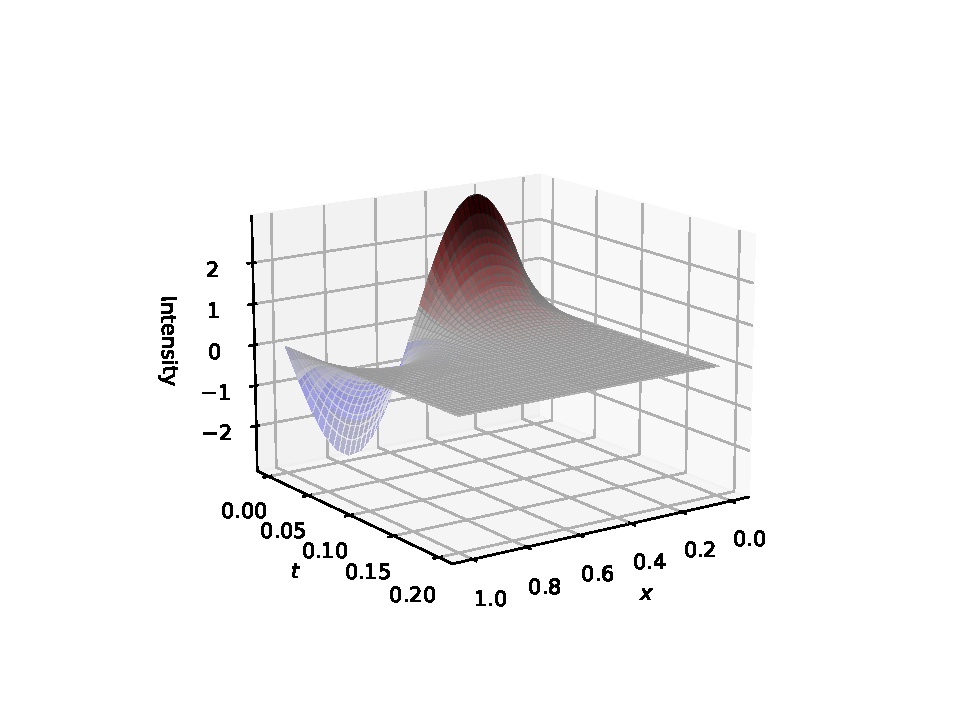
\includegraphics[width = 0.9\linewidth]{plots/2b_sol.pdf}
    \caption{Heat equation on $x \in [0,1]$ and $t \in [0,0.2]$ with homogeneous Dirichlet boundary conditions and initial condition $f(x)=3\sin{(2\pi x)}$. The numerical solution is calculated with CN with $M=N=20$ and plotted with a \textit{seismic} color map. The manufactured solution $u(x,t) = 3 e^{-4 \pi^2 t} \sin{(2 \pi x)}$ is plotted in grey.}
    \label{fig: 2b_sol}
\end{figure}

\subsubsection{Convergence Plots}
In the implementation of the numerical methods, both BE and CN are used to yield a method of second order in space, and first and second order in time, respectively (see equation \eqref{orders}). This means that the schemes \eqref{CN} and \eqref{BE}, with the matrix $Q$ on the form 

\begin{equation*}
Q = \begin{pmatrix}
    -2 & 1 & & & \\
    1 & -2 & 1 & & \\
    & \ddots & \ddots & \ddots &\\
     & & 1 & -2 & 1 \\
     &  & & 1 & -2
    \end{pmatrix}, 
\end{equation*}
are employed. 

\textcolor{red}{Les over dette senere ;)}
We shall consider four types of refinement, namely $h$-, $k$-, $(h=ck)$- and $r$-refinement. Their convergence rates is found by calculating the relative errors in both the $\ell_2$ and $L_2$ norm. The definitions for $e_{\ell}^r$ and $e_{L_2}^r$ can be found in section \ref{errors.section}. The errors are calculated with respect to the analytical solution \eqref{2b-analytical-solution} at the end time for our interval, $T=0.2$, every time the grid is refined. For each type of refinement do we calculate the convergence for both the BE and CN method.

First, $h$-refinement is performed. The convergence plot is depicted in figure \ref{2b_href}. As in problem 2 \mathbf{a)}, the error reaches a minimum when BE is used, due to the error in time. Nevertheless, it can be seen that the convergence is of order 2 when increasing $N$, which is expected from \eqref{orders}, because, in theory, $N$ is set to a large number ($N = 1000$ in the figure) such that the error in $t$ can be neglected, i.e. $\mathcal{O}(k^2 + h^2) = \mathcal{O}(h^2) = \mathcal{O}(N_{\mathrm{dof}}^{-2})$ and $\mathcal{O}(k + h^2) = \mathcal{O}(h^2) = \mathcal{O}(N_{\mathrm{dof}}^{-2})$ for CN and BE respectively. 

Next, $k$-refinement is performed. The convergence plot is depicted in figure \ref{2b_kref}. The convergence plot is in compliance with the truncation orders mentioned in equation \eqref{orders}. The theory predicts these convergence rates because, in theory, $M$ is set to a large number ($M = 1000$ in the figure), such that the error in $x$ can be neglected, i.e. $\mathcal{O}(k^2 + h^2) = \mathcal{O}(k^2) = \mathcal{O}(N_{\mathrm{dof}}^{-2})$ and $\mathcal{O}(k + h^2) = \mathcal{O}(k) = \mathcal{O}(N_{\mathrm{dof}}^{-1})$ for CN and BE respectively.

\begin{figure}
\centering
\subfloat[$h$-refinement]{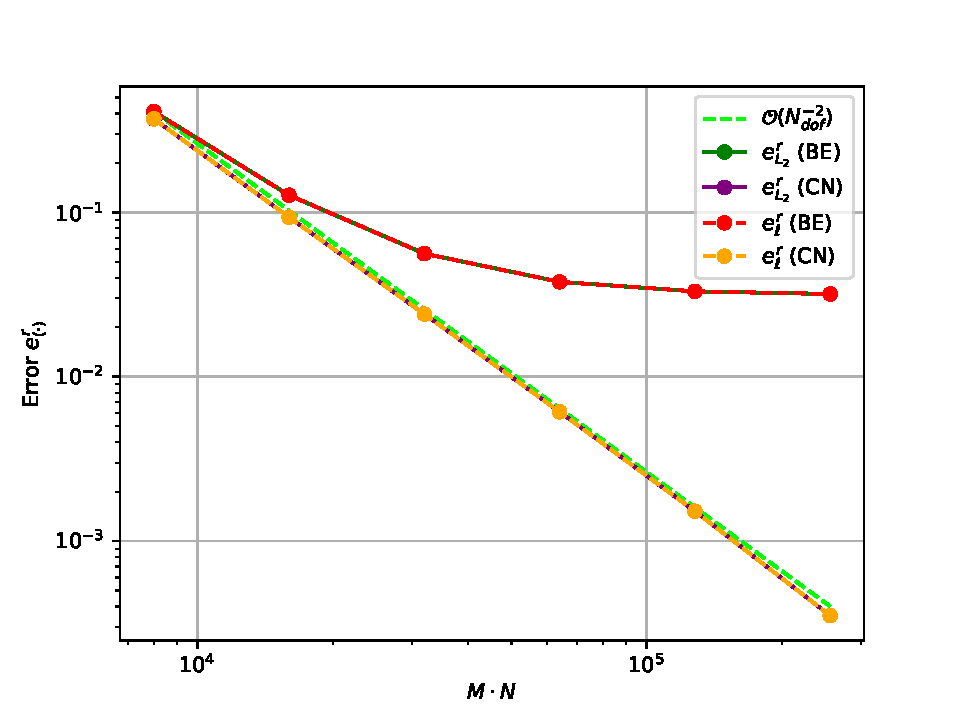
\includegraphics[width=0.85\linewidth]{plots/2b_href.pdf}\label{2b_href}}\hspace{0mm}
\subfloat[$k$-refinement]{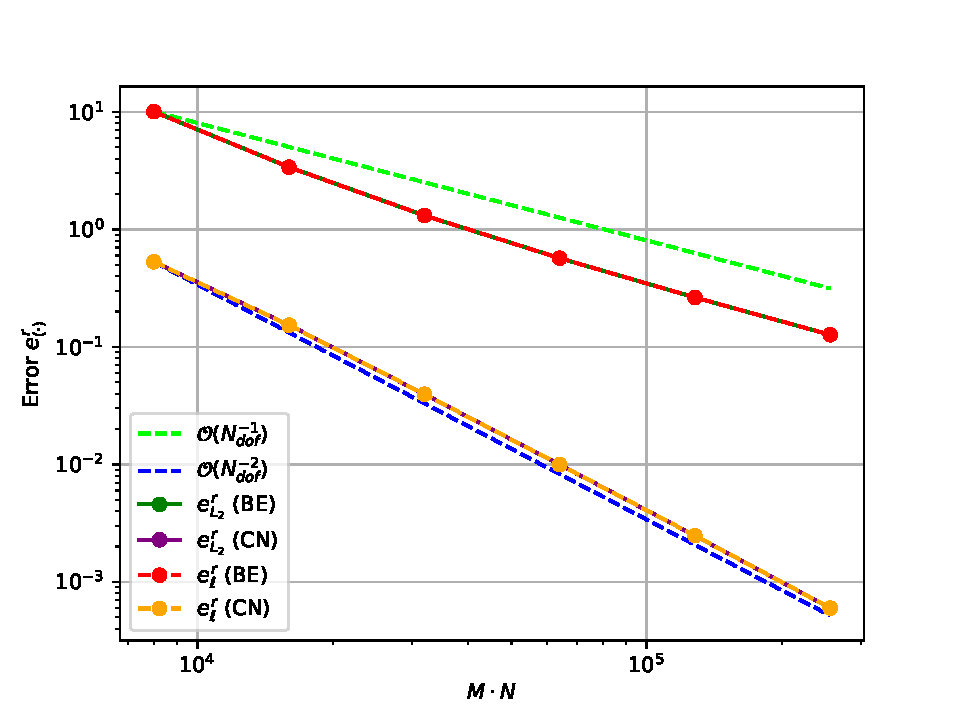
\includegraphics[width=0.85\linewidth]{plots/2b_kref.pdf}\label{2b_kref}}\hspace{0mm}
\caption{ Heat equation with homogeneous Dirichlet boundary conditions, with a manufactured solution $u(x,t) = 3 e^{-4 \pi^2 t} \sin{(2 \pi x)}$, on $x \in [0, 1]$ and $t \in [0, 0.2]$. The relative errors $e_\ell^r$ and $e_{L_2}^r$, obtained with $h$-refinement, are plotted in (a) with $N = 1000$. The relative errors, obtained with $k$-refinement, are plotted in (b) with $M = 1000$. Both BE and CN have been used as integrators. The $x$-axis shows $M \cdot N$, i.e. the number of degrees of freedom of the linear system.}
\end{figure}

Next, mesh refinement where $h = ck$, where $c := 1$, is performed.  From equation \eqref{orders}, it is expected that CN should yield a convergence of order $\mathcal{O}(k^2 + h^2) \overset{k \propto h} = \mathcal{O}(kh) = \mathcal{O}(N_{\mathrm{dof}}^{-1})$. On the other hand, BE is expected to yield convergence of order $\mathcal{O}(k + h^2) \overset{k \propto h} = \mathcal{O}(N_{\mathrm{dof}}^{-\frac{1}{2}} + N_{\mathrm{dof}}^{-1}) = \mathcal{O}(N_{\mathrm{dof}}^{-\frac{1}{2}} )$. The relative errors for both BE and CN are displayed in the convergence plot in figure \ref{2b_r1ref}, which shows that the expectations are met.

\begin{figure}
\centering
\subfloat[$(h = k)$-refinement]{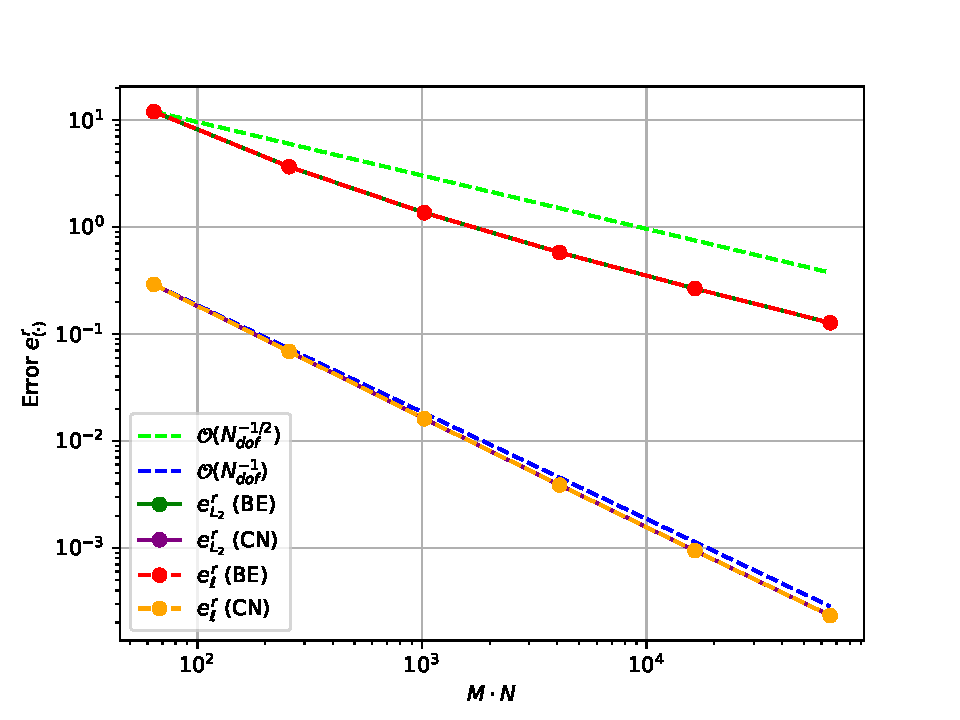
\includegraphics[width=0.85\linewidth]{plots/2b_r1ref.pdf}\label{2b_r1ref}}\hspace{0mm}\subfloat[Mesh refinement with $r = k/h^2$ constant]{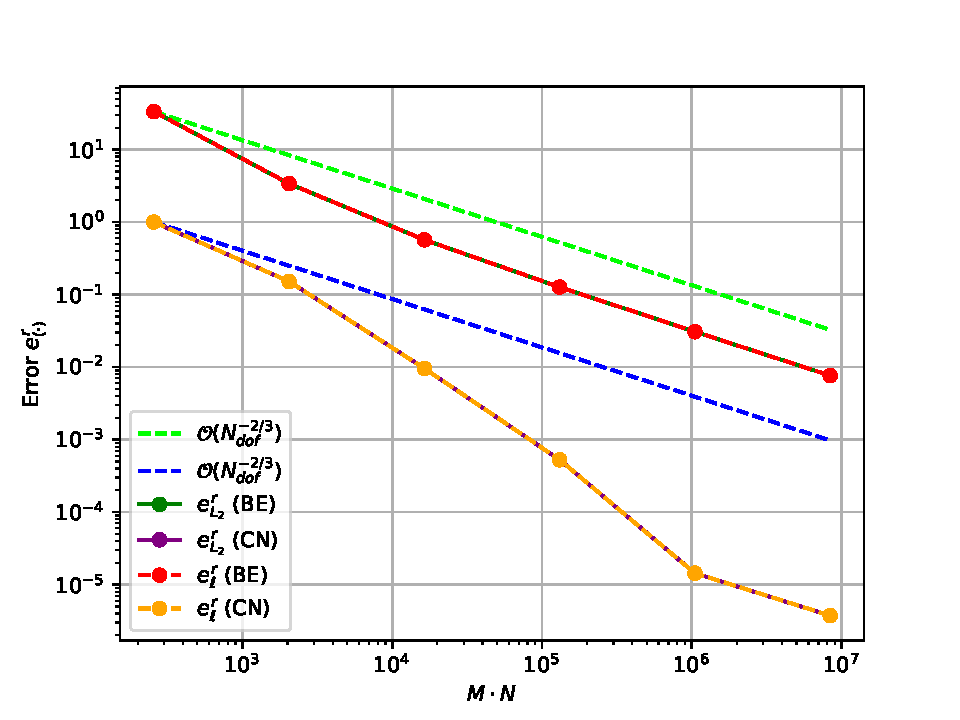
\includegraphics[width=0.85\linewidth]{plots/2b_r2ref.pdf}\label{2b_r2ref}}\hspace{0mm}
\caption{Heat equation with homogeneous Dirichlet boundary conditions, with a manufactured solution $u(x,t) = 3 e^{-4 \pi^2 t} \sin{(2 \pi x)}$, on $x \in [0, 1]$ and $t \in [0, 0.2]$. The relative errors $e_\ell^r$ and $e_{L_2}^r$, obtained with $(h = k)$-refinement, are plotted in (a). The relative errors, obtained with $r = k/h^2$-refinement, are plotted in (b). Both BE and CN have been used as integrators. The $x$-axis shows $M \cdot N$, i.e. the number of degrees of freedom of the linear system.}
\end{figure}

Finally, mesh refinement where $r = \frac{k}{h^2}$ is held constant, is performed. Notice that this implies that $k \propto h^2$ and hence $hk \propto h^3$. Thus, from equation \eqref{orders}, CN is expected to yield convergence of order

\begin{equation*}
    \begin{split}
        \mathcal{O}(k^2 + h^2) &\overset{k^2 \propto h^4}= \mathcal{O}(h^4 + h^2) \\ 
        = \mathcal{O}(h^2) &\overset{hk \propto h^3}= \mathcal{O}((hk)^{\frac{2}{3}}) = \mathcal{O}(N_{\mathrm{dof}}^{-\frac{2}{3}}).
    \end{split}
\end{equation*}
BE is expected to yield the same order of convergence

\begin{equation*}
    \begin{split}
        \mathcal{O}(k + h^2) &= \mathcal{O}(h^2) = \mathcal{O}((hk)^{\frac{2}{3}}) = \mathcal{O}(N_{\mathrm{dof}}^{-\frac{2}{3}}).
    \end{split}
\end{equation*}
The relative errors for both BE and CN are displayed in the convergence plot in figure \ref{2b_r2ref}, which shows that the expectations are partly met.

\newpage
\subsubsection{c)}
The inviscid Burgers' equation

\begin{equation}
    u_t = -uu_x, \, u(0,t) = u(1,t) = 0, \, u(x,0) = \exp{(-400(x-1/2)^2)},
\label{2c.burger}
\end{equation}
will be considered on $x \in [0,1], \, t > 0$. This is a special case of the parabolic Burgers' equation

\begin{equation*}
    u_t = \epsilon u_{xx} - uu_x, \, \epsilon \rightarrow 0.
\end{equation*}
The $x$-axis is discretized such that

\begin{equation*}
    x_0 = 0, \, x_1 = \frac{1}{M+1}, \, \dots, \, x_M = \frac{M}{M+1}, \, x_{M+1} = 1.
\end{equation*}
Let $v_m(t) \approx u(x_m,t)$ for $0 \leq m \leq M+1$ be the numerical solution along the line $(x_m,t)$. Using a central difference approximation for the first spatial derivative, which, from section \ref{section_2.2}, is known to be a second order approximation, leads to 

\begin{equation}
    \dot{v}_m =  - v_m\frac{1}{2h}(v_{m+1}-v_{m-1}), \quad 1 \le m \le M,
\label{burger_disc}
\end{equation}

\noindent All these differential equations can be written in vector format with $\boldsymbol{v}=[v_1,v_2,\dots,v_M]^T$. Combining the boundary conditions $v_0=v_{M+1}=0$  with \eqref{burger_disc} gives 

\begin{equation}
    \dot{\boldsymbol{v}} =: \boldsymbol{F}(\boldsymbol{v}) = \frac{1}{2h} \begin{pmatrix}
    -v_1v_2 \\
    \vdots \\
    -v_m(v_{m+1} - v_{m-1}) \\
    \vdots \\
    v_{M}v_{M-1}
    \end{pmatrix}
\label{2c.ODE}
\end{equation}

\noindent The system \eqref{2c.ODE} is solved in time with the ODE-solving method RK4. For a detailed description of the RK4 method see chapter 4. This yields a breaking time in the interval $t^* \in [0.057,0.060]$, which agrees with the theoretical value of $t^* = -1/ \min\{u'(x,0)\} \approx 0.0583$ found in \cite{Burgers}. Figure \ref{2c.fig} shows a visualization of the breaking point of the numerical solution. 

\begin{figure}[t]
    \centering
    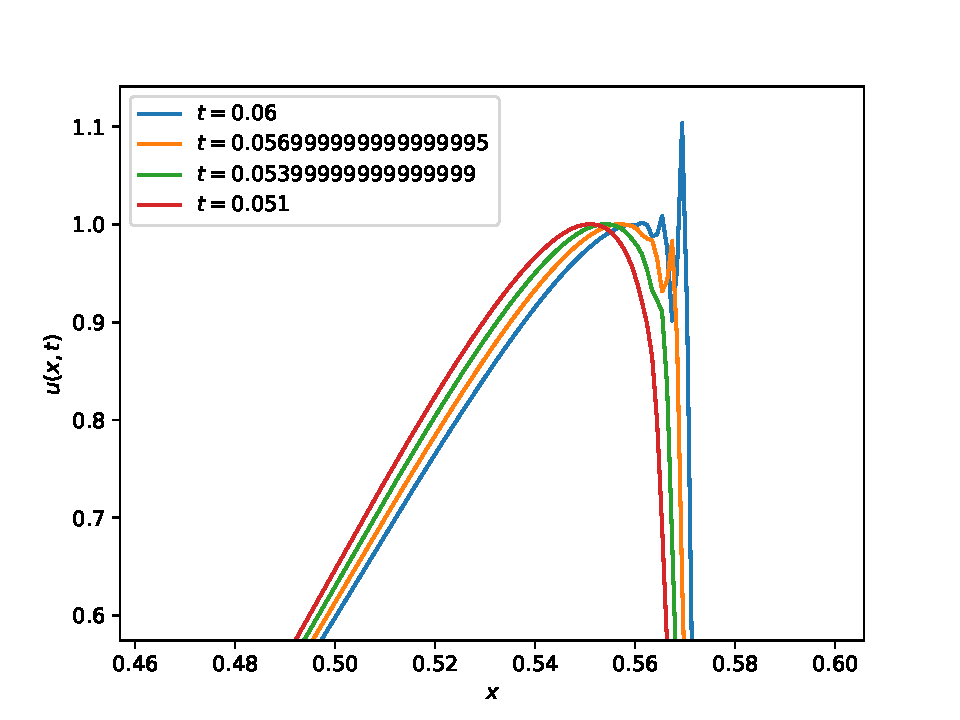
\includegraphics[width = 0.85\linewidth]{plots/2c.pdf}
    \caption{Inviscid Burger's equation on $x \in [0,1], \, t > 0$, with homogeneous Dirichlet boundary conditions and one initial condition. The numerical solution is plotted along the $x$-axis for different values of $t$. The plot illustrates the "breaking" behavior of the solution. }
    \label{2c.fig}
\end{figure}
\newpage
\ 
\newpage
\newpage
\ 
\newpage

\newpage

\section{Problem 3 - Laplace's Equation in Two Dimensions}
In this problem, the 2D Laplace equation on the unit square $(x,y) \in [0,1]^2 =: \Omega$, of the form 
\begin{equation}
\label{2DLaplace}
    \Delta u = u_{xx} + u_{yy} = 0, \hspace{1mm} u(x,y) = g(x,y) \hspace{1mm} \text{where} \hspace{1mm} (x,y) \in \partial \Omega, 
\end{equation}
is considered. The boundary condition $g(x,y)$ is given by 
\begin{equation*}
\begin{split}
    g(0,y) &= 0, \hspace{2mm} 0 \leq y \leq 1, \\
    g(x,0) &= 0, \hspace{2mm} 0 \leq x \leq 1, \\
    g(1,y) &= 0, \hspace{2mm} 0 \leq y \leq 1, \\
    g(x,1) &= \sin{(2\pi x)}, \hspace{2mm} 0 \leq x \leq 1. 
\end{split}
\end{equation*}

\subsubsection{a)}

The analytical solution of equation \eqref{2DLaplace} will be derived by using separation of variables \cite{Owren}. Suppose we are looking for solutions of the form $u(x,y) = X(x)Y(y)$. Inserted into the PDE \eqref{2DLaplace}, this assumption gives
\begin{equation*}
    X''(x)Y(y) + X(x)Y''(y) = 0.
\end{equation*}
This expression may be rearranged to 
\begin{equation*}
    \frac{X''(x)}{X(x)} = -\frac{Y''(y)}{Y(y)} = \lambda, 
\end{equation*}
since the variables $x$ and $y$ are separated. This means that both sides of the PDE must be a constant, denoted by $\lambda$. Hence, the PDE has been transformed into two separated ODE's
\begin{align}
    X''(x)-\lambda X(x) &= 0, \label{SeparatedX}\\
    Y''(y)+\lambda Y(y) &= 0. \label{SeparatedY}
\end{align}
The boundary conditions now become
\begin{align}
    g(0,y) &= X(0)Y(y) = 0, \hspace{2mm} 0 \leq y \leq 1, \label{BoundaryY1}\\
    g(1,y) &= X(1)Y(y) = 0, \hspace{2mm} 0 \leq y \leq 1, \label{BoundaryY2}\\
    g(x,0) &= X(x)Y(0) = 0, \hspace{2mm} 0 \leq x \leq 1, \label{BoundaryX1}\\
    g(x,1) &= X(x)Y(1) = \sin{(2\pi x)}, \hspace{2mm} 0 \leq x \leq 1. \label{BoundaryX2}
\end{align}

We begin by examining equation \eqref{SeparatedX}. The boundary conditions \eqref{BoundaryY1} and \eqref{BoundaryY2} give $X(0) = 0$ and $X(1) = 0$, assuming that $Y(y) \neq 0$, because that would lead to $u(x,y) = X(x)Y(y) = 0$, which is of no interest. When solving the equation \eqref{SeparatedX}, there are three different cases of the constant $\lambda$ we want to consider. Firstly, if $\lambda = 0$, the solution becomes a linear function $X(x) = A_1x+A_2$. The boundary conditions then give $A_2 = A_1 = 0$, which is uninteresting. Secondly, for positive $\lambda$, a general solution is $X(x) = A_1e^{\sqrt{\lambda}x} + A_2e^{-\sqrt{\lambda}x}$. Using the boundary conditions, this gives the linear system 
\begin{equation*}
\begin{split}
    X(0) &= A_1 + A_2 = 0, \\
    X(1) &= A_1e^{\sqrt{\lambda}} + A_2e^{-\sqrt{\lambda}} = 0, 
\end{split}
\end{equation*}
which still gives $A_1 = A_2 = 0$. Finally, if $\lambda$ is negative, say $\lambda = -k^2$, the general solution is $X(x) = A_1 \cos{kx} + A_2\sin{kx}$. Inserting the boundary conditions, the constants become $A_1 = 0$ and 
\begin{equation*}
    X(1) = A_2 \sin{k} = 0 \overset{A_2 \neq 0} \implies \sin{k} = 0 \implies k = n\pi \text{ for } n={\dots} -1,0,1, \dots .
\end{equation*}
Setting $A_2 = 1$ then gives infinitely many solutions $X(x) := X_n(x) = \sin{(n\pi x)}$, which satisfy $X''(x)-\lambda X(x) = 0$ when $\lambda := -k^2 = -n^2\pi^2$. 

Next, the solution of equation \eqref{SeparatedY} is be calculated. Inserting $\lambda := -k^2 = -n^2\pi^2$ gives $Y''(y)-n^2\pi^2Y(y) = 0$. A general solution of this equation is $Y(y) = B_1e^{n\pi y} + B_2e^{-n\pi y}$. Thus, the solution in $n$, determined up to the constants $B_1$ and $B_2$, is
\begin{equation*}
    \label{SeparatedWithConstants}
    u_n(x,y) = (B_1e^{n\pi y} + B_2e^{-n\pi y})\sin{(n\pi x)}.
\end{equation*}
Because the equation \eqref{2DLaplace} is linear and homogeneous, the superposition principle holds, which means that any linear combination of solutions to the PDE is also a solution. Hence, the infinite sum

\begin{equation}
    u(x,y) = \sum_{n=1}^\infty u_n(x,y) = \sum_{n=1}^\infty (B_1e^{n\pi y} + B_2e^{-n\pi y})\sin{(n\pi x)}
    \label{task3aInfiniteSumBeforeBCsFulfilled}
\end{equation}
is a solution of \eqref{2DLaplace}. Note that we only sum over $n \in [1, \infty)$ because $\sin{(-n\pi x)} = -\sin{(n\pi x)}$, which means that this sum incorporates the solutions for $n \in (\infty, 1)$ by means of a change in the coefficients $B_1$ and $B_2$. 

Two remaining boundary conditions still need to be satisfied. The boundary condition \eqref{BoundaryX1} gives 

\begin{equation*}
    0 = u(x,0) = \sum_{n=1}^\infty (B_1 + B_2)\sin{(n\pi x)}, 
\end{equation*}
which, by Fourier analysis, means that $B_1 + B_2 = \int_0^1 0\cdot \sin(n\pi x) \mathrm{d}x = 0$, which trivially gives $B_1 = -B_2$. Hence, this boundary condition is satisfied when the sum \eqref{task3aInfiniteSumBeforeBCsFulfilled} takes the form

\begin{equation*}
    u(x,y) = \sum_{n=1}^\infty B_1(e^{n\pi y} - e^{-n\pi y})\sin{(n\pi x)} = \sum_{n=1}^\infty B^*_n\sinh{(n\pi y)}\sin{(n\pi x)}, 
\end{equation*}
where $B^*_n = 2B_1$. The last boundary condition \eqref{BoundaryX2} gives

\begin{equation*}
    u(x,1) = \sum_{n=1}^\infty B^*_n\sinh{(n\pi)}\sin{(n\pi x)} = \sin{(2\pi x)}, 
\end{equation*}
which, by Fourier analysis, means that $B^*_n\sinh{(n\pi)}= 2\int_0^1\sin{(2\pi x)}\sin(n\pi x)\mathrm{d}x \implies B^*_n = \frac{2}{\sinh{(n\pi)}} \int_0^1\sin{(2\pi x)}\sin(n\pi x)\mathrm{d}x$. Hence, the analytical solution is given by

\begin{equation}
\begin{split}
    u(x,y) &= \sum_{n=1}^\infty B^*_n\sinh{(n\pi y)}\sin{(n\pi x)}, \\
     B^*_n &= \frac{2}{\sinh{(n\pi)}} \int_0^1\sin{(2\pi x)}\sin(n\pi x)\mathrm{d}x.
\end{split}
\label{task3aFinalSolutionBeforeCalcB}
\end{equation}
Next, the coefficients $B^*_n$ are calculated. From the expression of $B^*_n$ in \eqref{task3aFinalSolutionBeforeCalcB} it is apparent that

\begin{equation*}
\begin{split}
    B^*_2 &= \frac{2}{\sinh{(2\pi)}} \int_0^1\sin{(2\pi x)}\sin(2\pi x)\mathrm{d}x \\ 
    &= \frac{2}{\sinh{(2\pi)}} \cdot \frac12 = \frac{1}{\sinh{(2\pi)}}, 
\end{split}
\end{equation*}
is the only non-zero coefficient, since $\sin{(mx)}$ and $\sin{(nx)}$ are orthogonal functions when $m \neq n$. Hence, the final solution is 

\begin{equation}
    u(x,y) = \frac{1}{\sinh{(2\pi)}}\sinh{(2\pi y)}\sin{(2\pi x)}. 
\end{equation}

\subsubsection{b)}

In order to solve equation \eqref{2DLaplace} numerically, the five point formula 

\begin{equation}
    \delta_x^2U_p + \delta_y^2U_p = 0, 
    \label{fivePointFormula}
\end{equation}
where $p$ is the point in which the solution is to be found, is implemented on a grid. The $x$-axis is discretized as 

\begin{equation*}
    x_0 = 0, \, x_1 = \frac{1}{M_x+1}, \, \dots, \, x_{M_x} = \frac{M_x}{M_x+1}, \, x_{M_x+1} = 1,
\end{equation*}
and the $y$-axis is similarly discretized as 

\begin{equation*}
    y_0 = 0, \, y_1 = \frac{1}{M_y+1}, \, \dots, \, y_{M_y} = \frac{M_y}{M_y+1}, \, x_{M_y+1} = 1,
\end{equation*}
Constant step sizes $h = 1/(M_x+1)$ and $k = 1/(M_y+1)$ are used, where $M_x$ and $M_y$ are the number of internal nodes in the discretized grid in the $x$- and $y$-direction, respectively. In the general case, the five point formula yields

\begin{equation*}
    \frac{1}{h^2}(U_W - 2U_p + U_E) + \frac{1}{k^2}(U_S - 2U_p + U_N) = 0, 
\end{equation*}
where the cardinal directions north ($N$), south ($S$), east ($E$) and west ($W$) are shown in figure \ref{stencil} for a regular grid, i.e. $k = h$. When the grid is non-regular, the directions are still the same, but the lengths of the lines shown in figure \ref{stencil} will change. 

By traversing the $x$-axis from left to right, while traversing the $y$-axis from bottom to top, the five point stencil gives rise to a linear system $A\boldsymbol{U} = \boldsymbol{F}$. To illustrate, setting $M_x = M_y = 3$ gives 9 unknowns, and gives rise to the system 

\begin{equation*}
    A = \begin{pmatrix} 
    -4 & 1 & 0 & 1 & 0 & 0 & 0 & 0 & 0\\
    1 & -4 & 1 & 0 & 1 & 0 & 0 & 0 & 0 \\
    0 & 1 & -4 & 0 & 0 & 1 & 0 & 0 & 0\\
    1 & 0 & 0 & -4 & 1 & 0 & 1 & 0 & 0 \\
    0 & 1 & 0 & 1 & -4 & 1 & 0 & 1 & 0\\
    0 & 0 & 1 & 0 & 1 & -4 & 0 & 0 & 1\\
    0 & 0 & 0 & 1 & 0 & 0 & -4 & 1 & 0\\
    0 & 0 & 0 & 0 & 1 & 0 & 1 & -4 & 1 \\
    0 & 0 & 0 & 0 & 0 & 1 & 0 & 1 & -4\\
    \end{pmatrix}, \, 
    \boldsymbol{U} = \begin{pmatrix}
    U_1^1 \\
    U_1^2 \\
    U_1^3 \\
    U_2^1 \\
    U_2^2 \\
    U_2^3 \\
    U_3^1 \\
    U_3^2 \\
    U_3^3 \\
    \end{pmatrix}, \, \boldsymbol{F} = \begin{pmatrix}
    0 \\
    0 \\
    -\sin{(2\pi \frac14)} \\
    0 \\
    0 \\
    -\sin{(2\pi \frac12)} \\
    0 \\
    0 \\
    -\sin{(2\pi \frac34)} \\
    \end{pmatrix}, 
\end{equation*}
where the notation $U_{(\cdot)}^*$ encodes the solution in the $((\cdot), *)$-coordinate of the regular grid. Note that all the unknowns are internal points, since the boundary conditions are given. The solution to this system is shown in figure \ref{fig:task3M3}. Since the solution is very "non-smooth", i.e. a bad approximation of the analytical solution, more internal points need to be added to the grid. 

\tikzset{every label/.style={font=\footnotesize,inner sep=1pt}}
\newcommand{\stencilpt}[4][]{\node[circle,fill,draw,inner sep=1.5pt,label={above left:#4},#1] at (#2) (#3) {}}
\begin{figure}[t]
\centering
\begin{tikzpicture}
  \stencilpt{-2,0}{i-2}{$W$};
  \stencilpt{ 0,0}{i}  {$p$};
  \stencilpt{ 2,0}{i+2}{$E$};
  \stencilpt{0,-2}{j-2}{$S$};
  \stencilpt{0, 2}{j+2}{$N$};
  \draw 
        (j+2) -- (j-2)
        (i-2) -- (i+2);
\end{tikzpicture}
\caption{Five point stencil for the 2D Laplace equation, on a regular grid. }
\label{stencil}
\end{figure}

The linear system obviously changes when $M_x$ and $M_y$ change, but the manner in which the system is solved is similar. An example of a simple system where the grid is non-uniform is given next. Setting $M_y = 2$ and $M_x = 3$, gives $k = \frac{1}{3}$ and $h = \frac{1}{4}$. Then, the linear system is given by

\begin{equation*}
\begin{split}
    A = &\begin{pmatrix} 
    -2(\frac{1}{h^2}+\frac{1}{k^2}) & \frac{1}{k^2} & \frac{1}{h^2} & 0 & 0 & 0\\
    \frac{1}{k^2} & -2(\frac{1}{h^2}+\frac{1}{k^2}) & 0 & \frac{1}{h^2} & 0 & 0 \\
    \frac{1}{h^2} & 0 & -2(\frac{1}{h^2}+\frac{1}{k^2}) & \frac{1}{k^2} & \frac{1}{h^2} & 0 \\
    0 & \frac{1}{h^2} & \frac{1}{k^2} & -2(\frac{1}{h^2}+\frac{1}{k^2}) & 0 & \frac{1}{h^2} \\
    0 & 0 & \frac{1}{h^2} & 0 & -2(\frac{1}{h^2}+\frac{1}{k^2}) & \frac{1}{k^2} \\
    0 & 0 & 0 & \frac{1}{h^2} & \frac{1}{k^2} & -2(\frac{1}{h^2}+\frac{1}{k^2}) \\
    \end{pmatrix}, \\ &\boldsymbol{U} = \begin{pmatrix}
    U_1^1 \\
    U_1^2 \\
    U_2^1 \\
    U_2^2 \\
    U_3^1 \\
    U_3^2 \\
    \end{pmatrix}, \, \boldsymbol{F} = \begin{pmatrix}
    0 \\
    -\frac{1}{k^2}\sin{(2\pi \cdot h)} \\
    0 \\
    -\frac{1}{k^2}\sin{(2\pi \cdot 2h)} \\
    0 \\
    -\frac{1}{k^2}\sin{(2\pi \cdot 3h)} \\
    \end{pmatrix}, 
\end{split}
\end{equation*}
The solution of this system is not displayed, since it is very non-smooth, similarly to the previous example. Instead, as a visual confirmation of the similarities between the numerical and the analytical solution, figure \ref{task3M50} shows the solution with $M_x = M_y = 50$, i.e. 2500 internal grid points. The solution looks relatively smooth in this case. \newline 

\begin{figure}
\centering
\subfloat[$M_x = M_y = 3$]{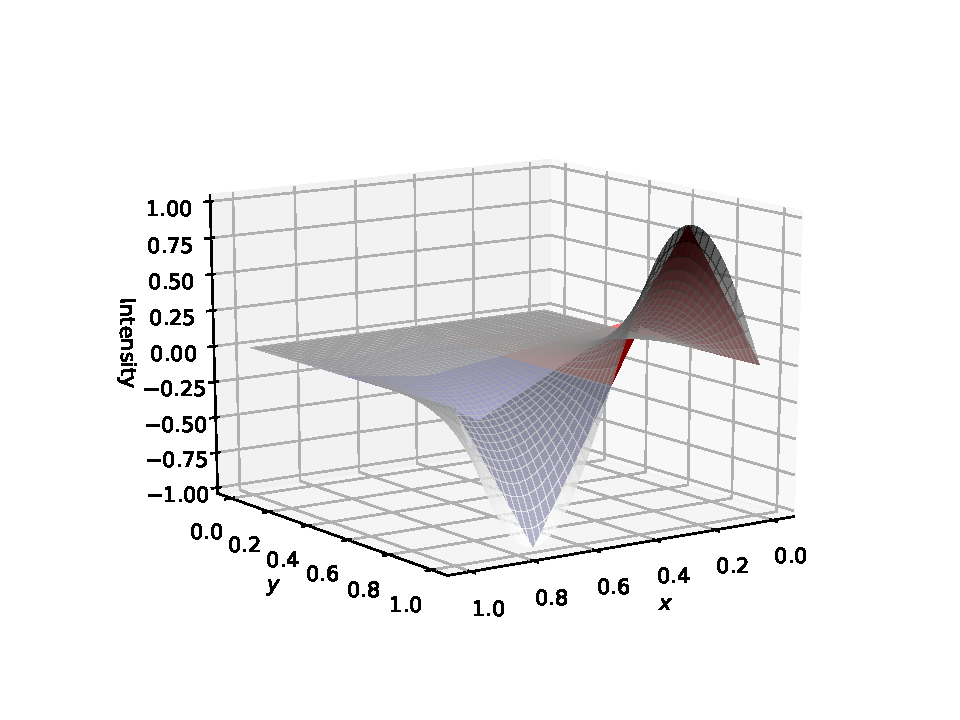
\includegraphics[width=0.9\linewidth]{plots/AnPlusNumSolM3Task3.pdf}\label{fig:task3M3}}\hspace{0mm}
\subfloat[$M_x = M_y = 50$]{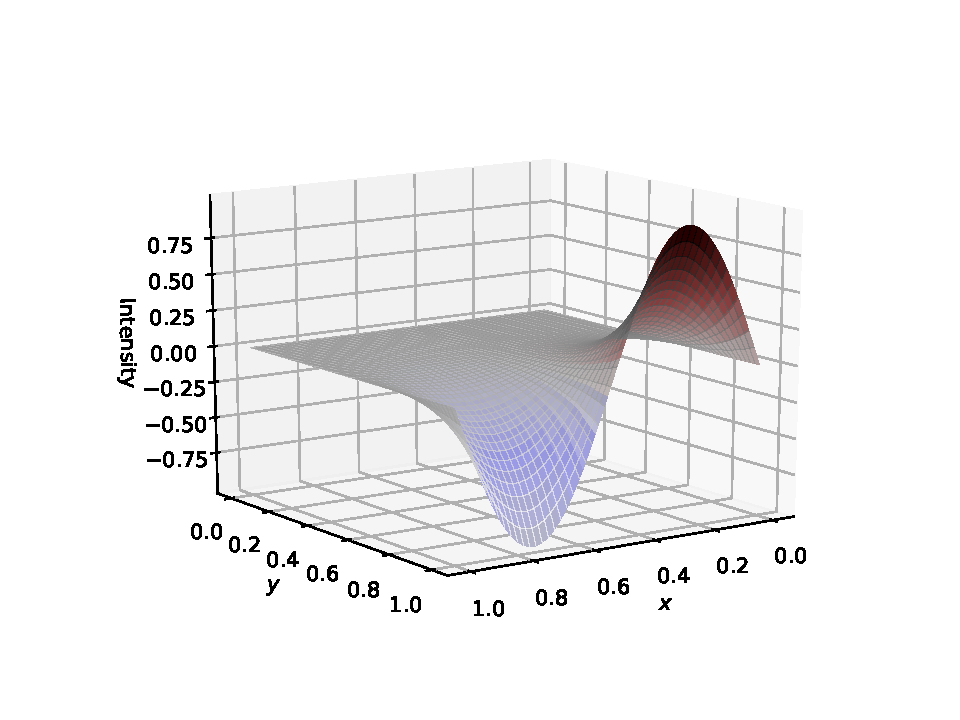
\includegraphics[width=0.9\linewidth]{plots/AnPlusNumSolM50Task3.pdf}\label{task3M50}}\hspace{0mm}
\caption{Two-Dimensional Laplace Equation, considered on the unit square. The analytical solution is shown in grey. The numerical solution is displayed in a \textit{seismic} color map. In (a), the numerical solution is calculated with $M_x = M_y = 3$, i.e. with 9 unknowns on a regular grid. In (b), the numerical solution is calculated with $M_x = M_y = 50$, i.e. with 2500 unknowns on a regular grid.}
\end{figure}
\newpage
In the next sections, the convergence of the numerical solution to the analytical solution will be quantified. Since the five point formula \eqref{fivePointFormula} uses a second order central difference approximation, as defined in section \ref{section_2.2}, in both directions $x$ and $y$, the truncation error is of order $\mathcal{O}(h^2 + k^2)$. The relative error $e^r_{\ell}$ for three different types of grids is displayed in "$\log$-$\log$"-convergence plots. The types of grids are 

\begin{itemize}
    \item $h$-refinement: $M_x$ increasing and $M_y$ constant
    \item $k$-refinement: $M_y$ increasing and $M_x$ constant
    \item $(h = k)$-refinement: Both $M_x$ and $M_y$ increasing at the same rate
\end{itemize}

\subsubsection*{Convergence with $h$-refinement}
Convergence plots for increasing $M_x$, with arbitrary constant values of $M_y$, are shown in figure \ref{subfigurestask3b1}. In all the cases presented, the convergence order is approximately $\mathcal{O}(N_{\mathrm{dof}}^{-2})$ up to a certain point, where the convergence order "flattens out". This matches the expected convergence rate, which is 

\begin{equation*}
\begin{split}
    \mathcal{O}(h^2 + k^2) &= \mathcal{O}(h^2) \overset{h \propto N_{\mathrm{dof}}^{-1}}= \mathcal{O}(N_{\mathrm{dof}}^{-2}), 
\end{split}
\end{equation*}
where $N_{\mathrm{dof}} = M_x\cdot M_y$. This is expected since $h$-refinement is being performed, which means that $k$ is assumed to be a small enough number such that $h$ will dominate the error. This is observed in practice when $M_x$ is increased. Note that the point where the convergence rate becomes asymptotic is shifted towards smaller errors and larger degrees of freedom when the constant $M_y$ is increased. This is clearly observed in the sequence of plots from (a) to (d). 

\begin{figure}[t]
\begin{subfigure}{.5\textwidth}
  \centering
  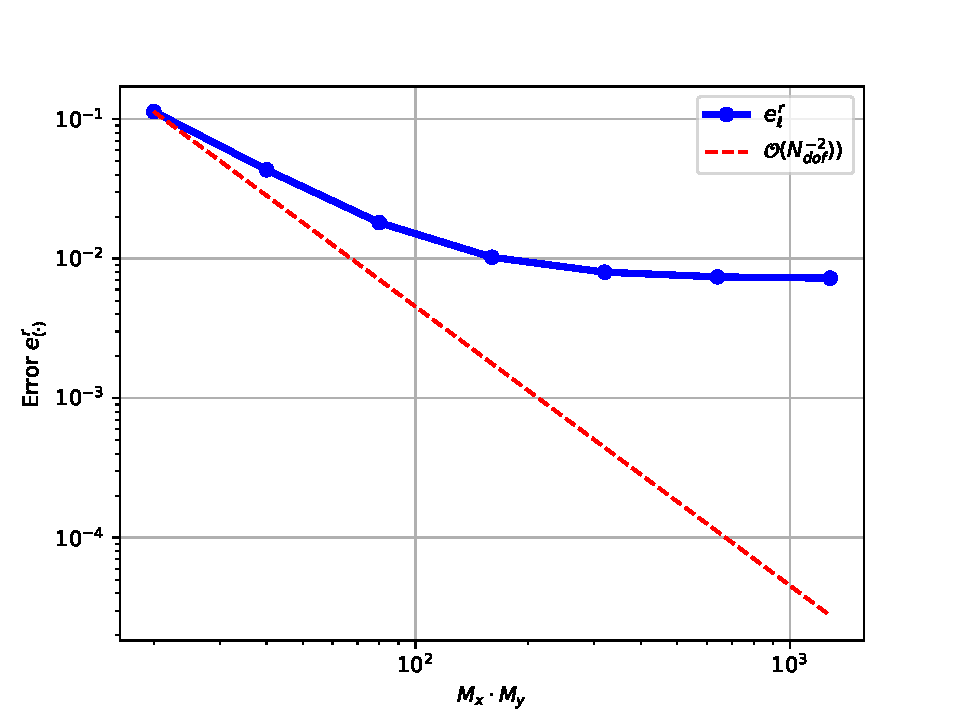
\includegraphics[width=\linewidth]{plots/task3bMy20.pdf}
  \caption{$M_y = 10$ and $M_x$ increasing}
\end{subfigure}
\begin{subfigure}{.5\textwidth}
  \centering
  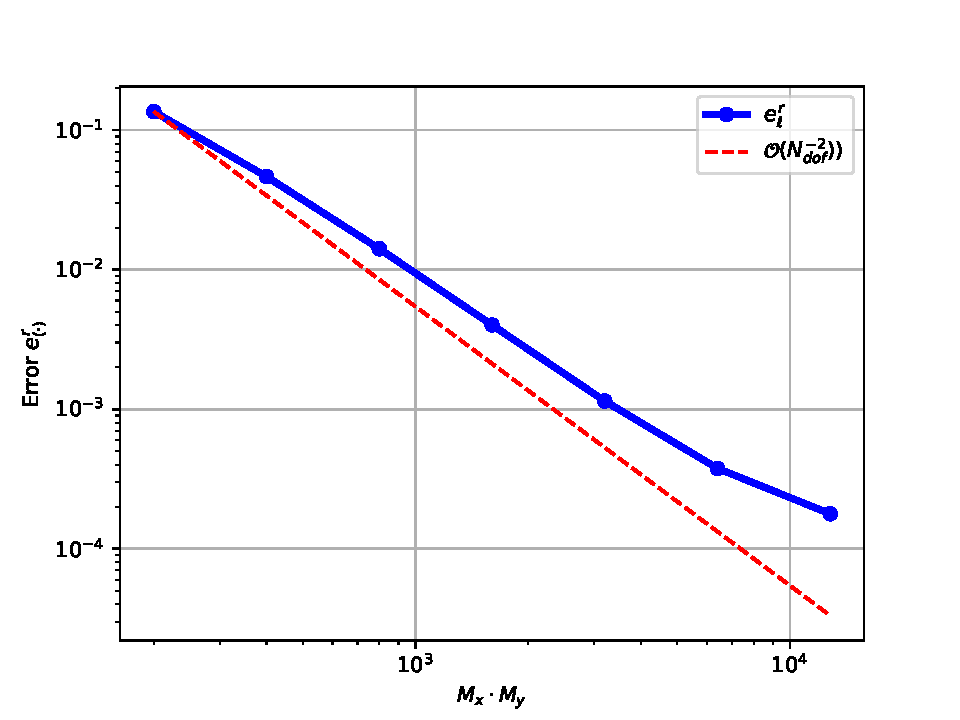
\includegraphics[width=\linewidth]{plots/task3bMy50.pdf}
  \caption{$M_y = 100$ and $M_x$ increasing}
\end{subfigure}
\begin{subfigure}{.5\textwidth}
  \centering
  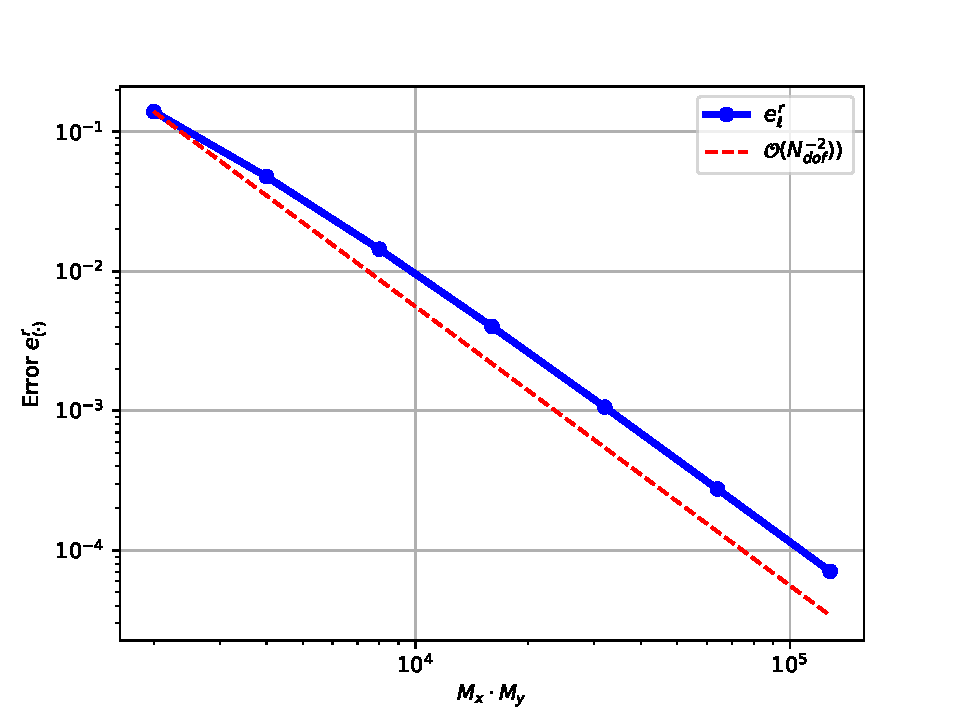
\includegraphics[width=\linewidth]{plots/task3bMy100.pdf}
  \caption{$M_y = 10^3$ and $M_x$ increasing}
\end{subfigure}
\begin{subfigure}{.5\textwidth}
  \centering
  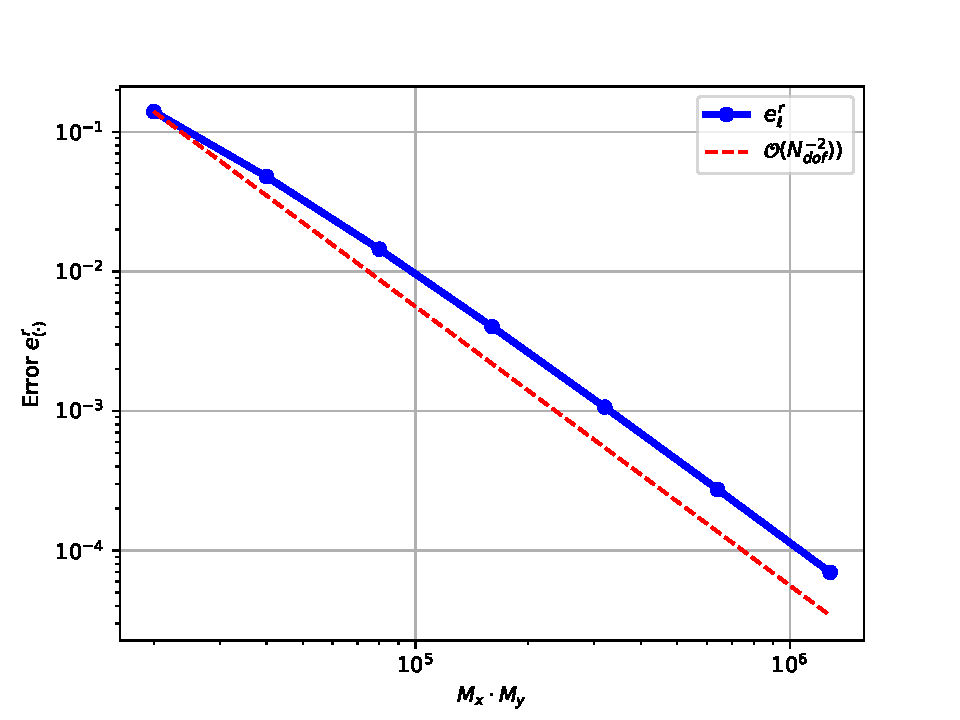
\includegraphics[width=\linewidth]{plots/task3bMy500.pdf}  \caption{$M_y = 10^4$ and $M_x$ increasing}
\end{subfigure}
\caption{Two-Dimensional Laplace Equation, considered on the unit square. The relative error $e^r_{\ell}$ is shown for some arbitrary constant values of $M_y$ and increasing $M_x$ ($h$-refinement). The $x$-axis shows $M_x \cdot M_y$, i.e. the number of degrees of freedom of the linear system.}
\label{subfigurestask3b1}
\end{figure}

\subsubsection*{Convergence with $k$-refinement}
Convergence plots for increasing $M_y$, with arbitrary constant values of $M_x$, are shown in figure \ref{subfigurestask3b2}. The expected convergence order, in this case, is

\begin{equation*}
\begin{split}
    \mathcal{O}(h^2 + k^2) &= \mathcal{O}(k^2) \overset{k \propto N_{\mathrm{dof}}^{-1}}= \mathcal{O}(N_{\mathrm{dof}}^{-2}). 
\end{split}
\end{equation*}
The reasoning of this expectation is similar as for $h$-refinement. In this case, $h$ is assumed to be a small number, such that the error stemming from $k$ will be asymptotically larger. In case (a) and (b), the expected convergence order of $\mathcal{O}(N_{\mathrm{dof}}^{-2})$ is not reached. The reason for this is that the constant $M_x$ is not large enough, which is assumed when neglecting the $h^2$-term when calculating the expected convergence order. Therefore, when the constant is increased, the expected convergence order is met, as observed in figures (c) and (d). Note that the point where the convergence rate becomes asymptotic is shifted towards larger errors and larger degrees of freedom when the constant $M_x$ is increased. Moreover, comparing to the plots in figure \ref{subfigurestask3b1}, it can be inferred that the refinement in the $x$-direction is crucial for reaching the expected convergence order. In other words, $x$ requires a finer grid compared to $y$. 

\begin{figure}[t]
\begin{subfigure}{.5\textwidth}
  \centering
  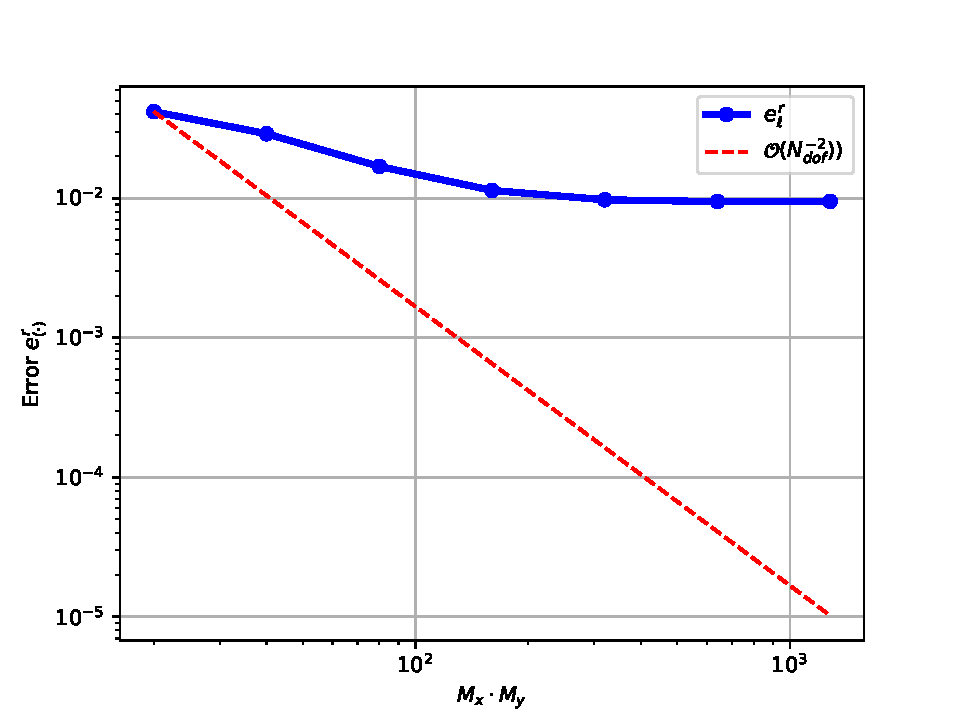
\includegraphics[width=\linewidth]{plots/task3bMx20.pdf}
  \caption{$M_x = 10$ and $M_y$ increasing}
\end{subfigure}
\begin{subfigure}{.5\textwidth}
  \centering
  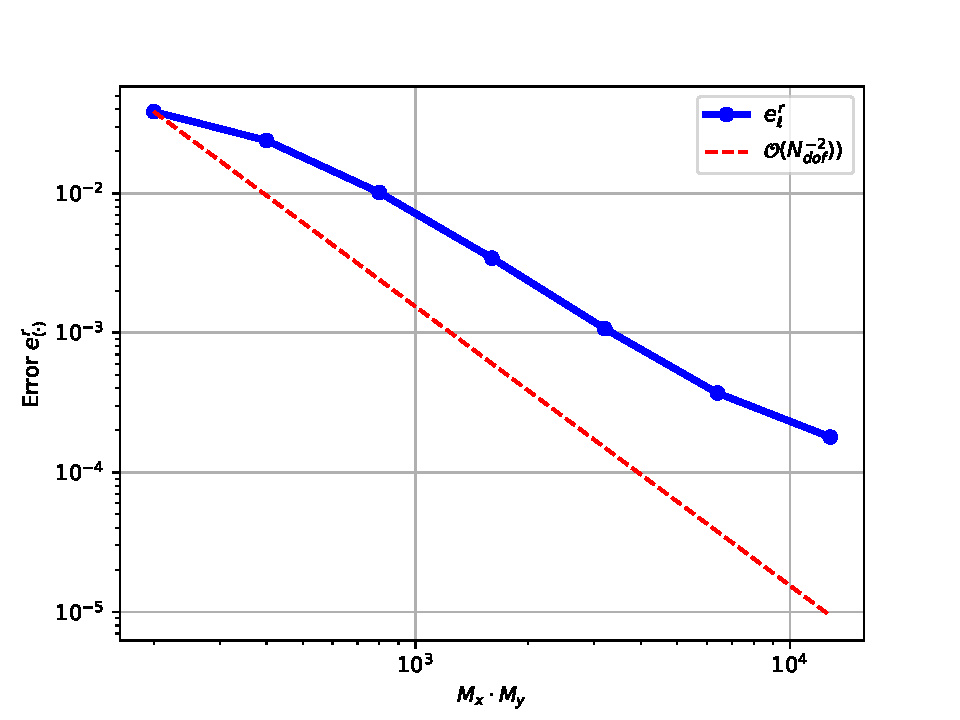
\includegraphics[width=\linewidth]{plots/task3bMx50.pdf}
  \caption{$M_x = 100$ and $M_y$ increasing}
\end{subfigure}
\begin{subfigure}{.5\textwidth}
  \centering
  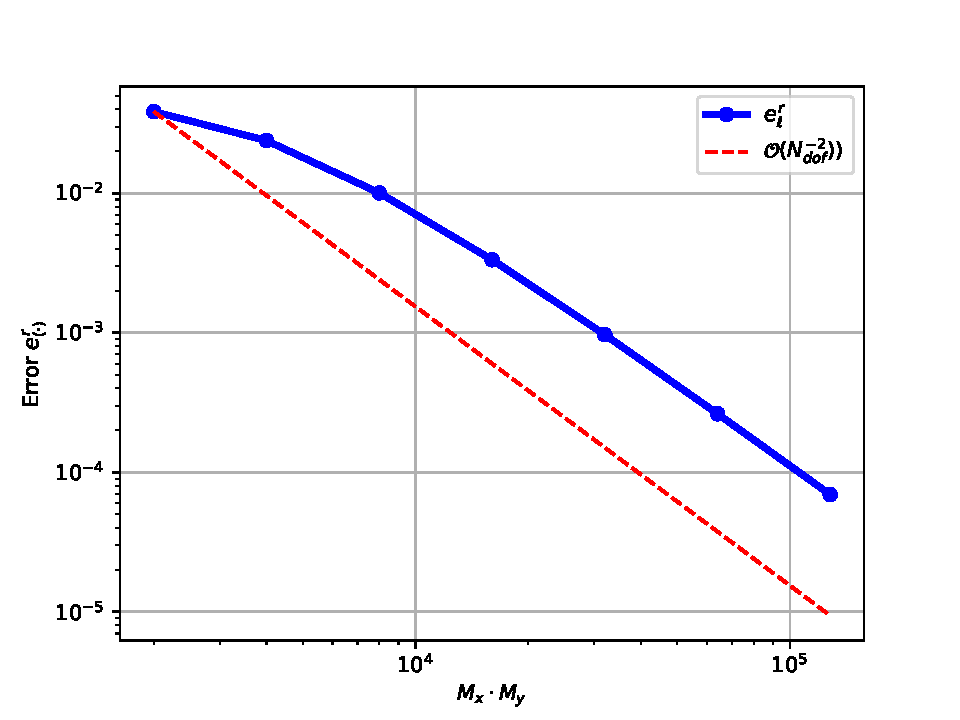
\includegraphics[width=\linewidth]{plots/task3bMx100.pdf}
  \caption{$M_x = 10^3$ and $M_y$ increasing}
\end{subfigure}
\begin{subfigure}{.5\textwidth}
  \centering
  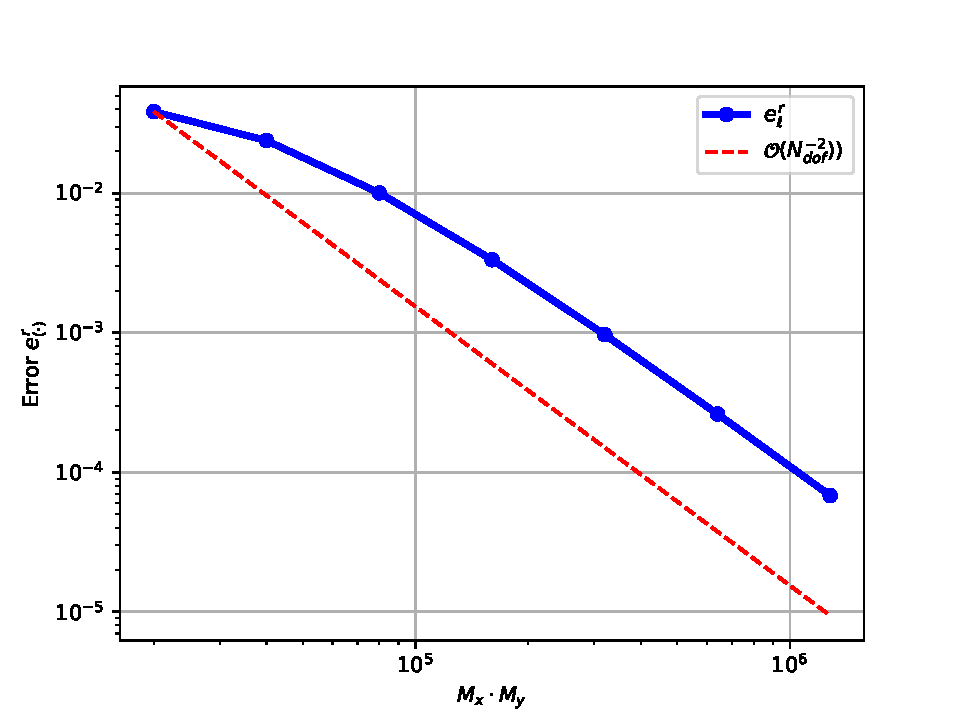
\includegraphics[width=\linewidth]{plots/task3bMx500.pdf}
  \caption{$M_x = 10^4$ and $M_y$ increasing}
\end{subfigure}
\caption{Two-Dimensional Laplace Equation, considered on the unit square. The relative error $e^r_{\ell}$ is shown for some arbitrary constant values of $M_x$ and increasing $M_y$ ($k$-refinement). The $x$-axis shows $M_x \cdot M_y$, i.e. the number of degrees of freedom of the linear system.}
\label{subfigurestask3b2}
\end{figure}

\subsubsection*{Convergence plot $(h = k)$-refinement}

A convergence plot where both $M_x$ and $M_y$ are increasing, at the same pace, i.e. $M_x = M_y$ at all times, is shown in figure \ref{task3bConvergenceBothVary}. As seen from the plot, the convergence order is approximately $\mathcal{O}(N_{\mathrm{dof}}^{-1})$. This is in accordance with the expected order of convergence, which is
\begin{equation*}
    \mathcal{O}(h^2+k^2) \overset{h = k} = \mathcal{O}(hk) = \mathcal{O}(N_{\mathrm{dof}}^{-1}).
\end{equation*}

\begin{figure}[t]
    \centering
    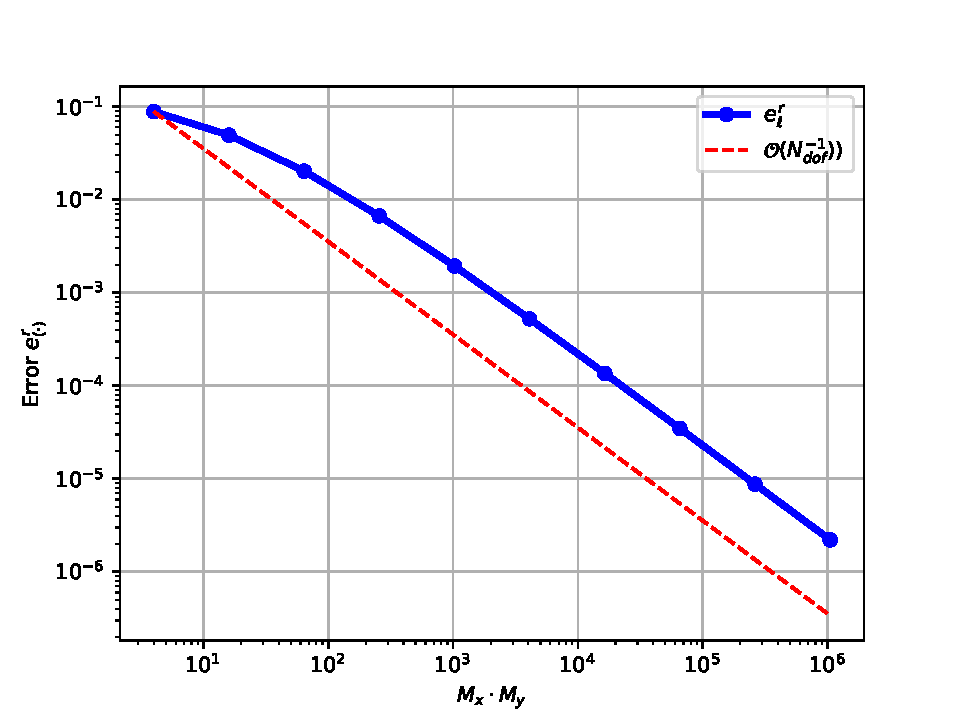
\includegraphics[width=0.85\linewidth]{plots/task3bBothVary.pdf}
    \caption{Two-Dimensional Laplace Equation, considered on the unit square. Plot of the relative error $e^r_{\ell}$ where both $M_x$ and $M_y$ are increasing monotonically ($(h=k)$-refinement). The $x$-axis shows $M_x \cdot M_y$, i.e. the number of degrees of freedom of the linear system.}
    \label{task3bConvergenceBothVary}
\end{figure}
\newpage
\ 
\newpage
\newpage
\ 
\newpage

\newpage

\section{Problem 4 - Linearized Korteweg-deVries Equation}
In this problem, the following linearized Korteweg-deVries (KdV) equation is considered on the interval $x \in [-1, 1], \hspace{1mm} t > 0, $

\begin{equation}
\label{KdV}
    u_t + (1+\pi^2)u_x + u_{xxx} = 0, \hspace{1mm} u(x,0) = \sin{(\pi x)}.
\end{equation}
A periodic boundary condition with period 2, i.e. $u(x+2, t) = u(x,t)$, is assumed. Hence, the function may be studied only on the interval $[-1, 1]$. The grid points

\begin{equation*}
    x_0 = -1, \, x_1 = -1 + \frac{2}{M}, \, \dots, \, x_M = 1,
\end{equation*}
are considered.

\subsubsection{a)}
In order to solve equation \eqref{KdV} numerically, it has to be discretized in time and space. Let $u_m^n := u(x_m,t_n)$ where $x_m=-1+mh \text{,  } 0 \leq m \leq M$ and $h=\frac{2}{M}$. The central difference approximation for the first derivative defined in \eqref{Theory_approx_first_derivative} in section \ref{section_2.2} is used to approximate the first spatial derivative. Thus, the approximation of $(u')_m:=u_x(x_m)$ at time step $t=t_n$ is

\begin{equation}
\begin{split}
\label{task4firstdisc}
 (u')_m &= \frac{1}{h} \mu \delta_x u_m + \mathcal{O}(h^2) \\ &= \frac{1}{2h} \left(u_{m+1} - u_{m-1}\right) + \mathcal{O}(h^2).
\end{split}
\end{equation}
Similarly, a discrete approximation for the third derivative $(u''')_m:=u_{xxx}(x_m)$ at $t=t_n$ is

\begin{equation}
\begin{split}
\label{task4thirdisc}
 (u''')_m &= \frac{1}{h^3} (\mu \delta_x)^3 u_m + \mathcal{O}(h^2) = \frac{1}{2h^3} (\mu \delta_x)^2 \left(u_{m+1}-u_{m-1}\right) + \mathcal{O}(h^2) \\ &= \frac{1}{4h^3} \mu \delta_x \left(u_{m+2}-2u_m + u_{m-2}\right) + \mathcal{O}(h^2) \\ &= \frac{1}{8h^3} \left(u_{m+3}-3u_{m+1}+3u_{m-1}-u_{m-3}\right) + \mathcal{O}(h^2). 
\end{split}
\end{equation}
Both these discretizations have a local truncation error of $\mathcal{O}(h^2)$. For the discretization in the temporal direction, both Euler's method and the Crank-Nicolson (trapezoidal) method are used. \newline

The temporal discretization using Euler's method can be derived as follows. The step size in the temporal direction is denoted by $k$. An expansion of the exact solution $u_m^{n+1}$ for constant $x = x_m$ around $t = t_n$ yields 

\begin{equation*}
\begin{split}
    u_m^{n+1} &= u_m^n + k \partial_tu_m^n + \frac12k^2\partial^2_tu_m^n + \dots \\ 
    &= u_m^n - k((1+\pi^2)(u')_m + (u''')_m) + \mathcal{O}(k^2), 
\end{split}
\end{equation*}
where equation \eqref{KdV} has been used in the second equality. Now, inserting the two spacial discretizations \eqref{task4firstdisc} and \eqref{task4thirdisc} gives

\begin{equation}
\begin{split}
\label{task4EulerExact}
    u_m^{n+1} &= u_m^n - k((1+\pi^2)(u')_m + (u''')_m) + \mathcal{O}(k^2)\\ 
    &= u_m^n - k\left(\frac{1+\pi^2}{2h}(u_{m+1}^n - u_{m-1}^n) + \frac{1}{8h^3}(u_{m+3}^n - 3u_{m+1}^n + 3u_{m-1}^n - u_{m-3}^n)\right) \\& \hspace{10mm} + \mathcal{O}(k^2 + kh^2)\\
    &= u_m^n - \frac{k}{2h}\left(\frac{1}{4h^2}u_{m+3}^n+\left[1+\pi^2 - \frac{3}{4h^2}\right]u_{m+1}^n-\left[1+\pi^2 - \frac{3}{4h^2}\right]u_{m-1}^n-\frac{1}{4h^2}u_{m-3}^n\right) \\& \hspace{10mm} + \mathcal{O}(k^2 + k h^2),
\end{split}
\end{equation}
which has a truncation error, $\tau_m^n$, of order $\mathcal{O}(k + h^2)$, since $k\tau_m^n = \mathcal{O}(k^2 + kh^2)$. The notation $U_m^n$ is adopted to specify the approximate solution of $u_m^n$, i.e. in the point $(x_m, t_n)$. Inserting this approximate solution into the equation \eqref{task4EulerExact} and neglecting the truncation error yields the difference scheme 

\begin{equation}
\label{task4discEuler}
    U_m^{n+1} = U_m^n + k\left(-aU_{m+3}^n-b U_{m+1}^n+bU_{m-1}^n+aU_{m-3}^n\right),
\end{equation}
where the coefficients $a$ and $b$ are defined as

\begin{equation}
\label{constants_spatialdiscretization}
    a = \frac{1}{8h^3} \text{,} \hspace{4mm}
    b = \frac{1+\pi^2}{2h} - \frac{3}{8h^3}.
\end{equation}
\newline

Crank-Nicolson is based on the trapezoidal rule, which gives a slightly different derivation of the temporal discretization when using this method. The fundamental theorem of calculus, together with the trapezoidal quadrature, yield

\begin{equation*}
\begin{split}
    u(x_m, t_{n+1}) - u(x_m, t_n) & = \int_{t_n}^{t_{n+1}} u_t(x_m, t)\mathrm{d}t \\
    &= \frac{t_{n+1}-t_n}{2} \left(u_t(x_m,t_{n+1}) + u_t(x_m,t_n))\right) + \mathcal{O}((t_{n+1}-t_n)^3) \\
    &= \frac{1}{2}k \left(u_t(x_m,t_{n+1})+u_t(x_m,t_n))\right) + \mathcal{O}(k^3).
\end{split}
\end{equation*}
This expression, together with the (KdV)-equation \eqref{KdV}, leads to 

\begin{equation}
\begin{split}
    u_m^{n+1} &= u_m^n + \frac12k(\partial_tu_m^n + \partial_tu_m^{n+1}) + \mathcal{O}(k^3) \\
    &= u_m^n - \frac12k((1+\pi^2)(u')_m^{n} + (u''')_m^{n}+(1+\pi^2)(u')_m^{n+1} + (u''')_m^{n+1}) + \mathcal{O}(k^3) \\
    &= u_m^n - \frac12k((1+\pi^2)((u')_m^{n} + (u')_m^{n+1}) + (u''')_m^{n} + (u''')_m^{n+1}) + \mathcal{O}(k^3), 
\end{split}
\end{equation}
where the $\mathcal{O}(k^3)$-error stems from the trapezoidal quadrature. Also, a superscript $n$ or $n+1$ is added to the derivative approximations, to signal at which point in time the functions are evaluated. Inserting the two spacial discretizations \eqref{task4firstdisc} and \eqref{task4thirdisc} yields

\begin{equation}
\begin{split}
\label{task4CrankExact}
    u_m^{n+1} &= u_m^n - \frac12k((1+\pi^2)((u')_m^{n} + (u')_m^{n+1}) + (u''')_m^{n} + (u''')_m^{n+1}) + \mathcal{O}(k^3) \\
    &= u_m^n - \frac12k\left(\frac{1+\pi^2}{2h}(u_{m+1}^n - u_{m-1}^n + u_{m+1}^{n+1} - u_{m-1}^{n+1}) \right.\\ &\left.+ \frac{1}{8h^3}(u_{m+3}^n - 3u_{m+1}^n + 3u_{m-1}^n - u_{m-3}^n + u_{m+3}^{n+1} - 3u_{m+1}^{n+1} + 3u_{m-1}^{n+1} - u_{m-3}^{n+1})\right) + \mathcal{O}(k^3 + k h^2)\\
    &= u_m^n + \frac{k}{2}\left( \frac{1}{8h^3}(-u_{m+3}^{n+1} + u_{m-3}^{n+1}-u_{m+3}^n + u_{m-3}^n) \right.\\ &\left.+ \left(\frac{1+\pi^2}{2h}-\frac{3}{8h^3}\right) (-u_{m+1}^{n+1} + u_{m-1}^{n+1}-u_{m+1}^n+u_{m-1}^n) \right) + \mathcal{O}(k^3 + k h^2).
\end{split}
\end{equation}
Finally, insertion of the approximate solution $U$ into the equation \eqref{task4CrankExact}, while neglecting the truncation error, and making use of the coefficients defined in \eqref{constants_spatialdiscretization}, gives the difference scheme 

\begin{equation}
\begin{split}
\label{task4discCrank}
    U_m^{n+1} = U_m^n + \frac{k}{2}\left(-a U_{m+3}^{n+1} - b U_{m+1}^{n+1} + b U_{m-1}^{n+1} + a U_{m-3}^{n+1} - a U_{m+3}^n - b U_{m+1}^n + b U_{m-1}^n +a U_{m-3}^n \right).
\end{split}
\end{equation}

\subsubsection*{Von Neumann stability}
Next in line is to examine if these two discretization methods are Von Neumann stable. The discretization based on Euler's method \eqref{task4discEuler} is examined first. Assume solutions of the form $U_m^n = \xi^n \mathrm{e}^{i\beta x_m}$ with $x_m = -1 + mh$. Insertion into the discretization formula yields an equation where all the terms contain the expression $\mathrm{e}^{-i\beta}$. Dividing the equation by this exponential expression yields 

\begin{equation*}
    \xi^{n+1} \mathrm{e}^{i\beta mh} = \xi^n \mathrm{e}^{i\beta mh} + k\xi^n (-a \mathrm{e}^{i\beta (m+3)h} - b\mathrm{e}^{i\beta (m+1)h} +b\mathrm{e}^{i\beta (m-1)h} +a \mathrm{e}^{i\beta (m-3)h}).
\end{equation*}
Moreover, dividing the equation by $\xi^n \mathrm{e}^{i\beta m h}$ leads to 

\begin{equation*}
\begin{split}
    \xi &= 1 + k(-a \mathrm{e}^{3 i\beta h} - b \mathrm{e}^{i\beta h} + b\mathrm{e}^{-i\beta h} + a\mathrm{e}^{-3 i\beta h}) \\
    &= 1 - 2ki(a \sin{(3 \beta h)} + b \sin{(\beta h)}).\\
\end{split}
\end{equation*}
Now, using the fact that $\sin{(3x)} = 3\sin{(x)} - 4\sin^3{(x)}$ and that $b = \frac{1+\pi^2}{2h} - 3a$, yields

\begin{align}
    \xi &= 1 - 2ki\left(3a\sin{(\beta h)}-4a\sin^3{(\beta h)}+\left(\frac{1+\pi^2}{2h}-3a\right)\sin{(\beta h)}\right) \nonumber\\
    &= 1 -2ki\left(\left(\frac{1+\pi^2}{2h}\right)\sin{(\beta h)}-4a\sin^3{(\beta h)}\right)\nonumber \\
    &= 1 + i\frac{k}{h}\sin{(\beta h)} \left(\frac{\sin^2{(\beta h)}}{h^2}-(1+\pi^2)\right),
    \label{xiEulerTask4a}
\end{align}
where $a=\frac{1}{8h^3}$ has been inserted in the last step. To achieve Von Neumann stability, the condition $|\xi| \leq 1 + \mu k$, where $\mu \geq 0$ is a constant independent of $h$ and $k$, needs to be satisfied. The Von Neumann stability criterion is equivalently stated as 

\begin{equation*}
    |\xi|^2 \leq 1 + 2\mu k + (\mu k)^2.
\end{equation*}
The squared modulus of equation \eqref{xiEulerTask4a} is given as
\begin{align*}
    |\xi|^2 &= 1 + \frac{k^2}{h^2}\sin^2{(\beta h)} \left(\frac{\sin^2{(\beta h)}}{h^2}-(1+\pi^2)\right)^2 \nonumber \\ &= 1 + k^2 \beta_h^2 \left(\beta_h^2 - C^2\right)^2,
    %\label{xi^2Euler}
\end{align*}
where the quantities $C:=\sqrt{1+¨\pi^2}$ and $\beta_h:=\frac{\sin{(\beta h)}}{h}$ are defined. Assuming (by contradiction) that the Von Neumann criterion is satisfied gives

\begin{equation*}
    \begin{split}
        & 2\mu k + \mu^2 k^2 -k^2 \beta_h^2 \left(\beta_h^2 - C^2\right)^2 \geq 0\\ & \Rightarrow \mu^2 k^2 + 2\mu k - k^2 \beta_h^2\left(\beta_h^2 -C^2\right)^2 = D \text{,} \hspace{2mm} D \geq 0 \\ \text{(abc-formula) }&\Rightarrow \mu = \frac{1}{k} \left(-1 \pm \sqrt{1 + D + k^2 \beta_h^2 (\beta_h^2-C^2)^2}\right).
    \end{split}
\end{equation*}
Observe that it is possible for $\mu$ to be a non-negative constant if the positive solution of the quadratic formula is chosen. Furthermore, independence of $\mu$ from $h$ and $k$ is only possible if $\mu=0$. These observations yield

\begin{equation*}
    \begin{split}
        &\mu = 0 \Rightarrow -1 + \sqrt{1 + D + k^2 \beta_h^2 (\beta_h^2-C^2)^2} = 0 \\ & \Rightarrow D = -k^2 \beta_h^2(\beta_h^2-C^2)^2.
    \end{split}
\end{equation*}
The last equation is clearly a contradiction to the criterion that $D \geq 0$. Hence, there exists no positive constant $\mu$ independent of $h$ and $k$ that satisfies the Von Neumann criterion. Conclusively, the discretization based on Euler's method \eqref{task4discEuler} is not Von Neumann stable. 
\begin{comment}
\textcolor{red}{The old version;}
For Euler's method, such a constant $\mu$ does not exist, because

\begin{align}
    |\xi|^2 &= 1 + \frac{k^2}{h^2}\sin^2{(\beta h)} \left(\frac{\sin^2{(\beta h)}}{h^2}-(1+\pi^2)\right)^2 \nonumber \\
    &= 1 + \frac{k^2}{h^2}\sin^2{(\beta h)}\left(\frac{\sin^4{(\beta h)}}{h^4} - 2\frac{\sin^2{(\beta h)}}{h^2}(1+\pi^2) + (1+\pi^2)^2\right) \nonumber \\
    &= 1 + \frac{k^2}{h^2}\sin^2{(\beta h)}\left(\frac{\sin^4{(\beta h)}}{h^4} - 2\frac{\sin^2{(\beta h)}}{h^2}C + C^2\right),
    \label{xi^2Euler}
\end{align}
where the constant value $C = (1+\pi^2)$ is highlighted by redefinition. It is apparent that it is impossible to bound \eqref{xi^2Euler} by $1 + 2\mu k + (\mu k)^2$, since a constant $\mu \geq 0$ independent of $h$ and $k$ is not possible to define. In fact, asymptotically, the expression \eqref{xi^2Euler}  is bounded by $u = 1 + \mathcal{O}(h^{-6})$, where $u \overset{h \rightarrow 0} \longrightarrow \infty$. The forward Euler method \eqref{task4discEuler} is therefore not Von Neumann stable.\textcolor{red}{stop old version.} \newline
\end{comment}

Next, the discretization based on Crank-Nicolson \eqref{task4discCrank}, is examined. In a similar manner, it is assumed that $U_m^n = \xi^n \mathrm{e}^{i\beta x_m}$ and $x_m = -1 + mh$. Insertion into the discretization formula and dividing the equation by $\xi^n \mathrm{e}^{i \beta m h}\mathrm{e}^{-i\beta}$ yields

\begin{equation*}
\begin{split}
    \xi  &= 1+ \frac{k}{2} \left(-a\xi \mathrm{e}^{3i \beta h} -b\xi \mathrm{e}^{i \beta h} + b\xi \mathrm{e}^{-i \beta h}+a\xi \mathrm{e}^{-3 i \beta h} - a\mathrm{e}^{3i \beta h}-b\mathrm{e}^{i \beta h}+b\mathrm{e}^{-i \beta h}+a\mathrm{e}^{-3i \beta h}\right)\\
    &= 1 -k i\left(a\xi \sin{(3 \beta h)} +b\xi \sin{(\beta h)} + a\sin{(3\beta h)}+b\sin{(\beta h)} \right)\\ \vspace{2mm}
    &\Rightarrow \xi + k i \xi \left(a \sin{(3\beta h)}+b\sin{(\beta h)}\right) = 1 - ki\left(a\sin{(3\beta h)+b\sin{(\beta h)}} \right)\\
    &\Rightarrow \xi = \frac{1 -ki\left(a \sin{(3\beta h)}+b\sin{(\beta h)}\right)}{1+ki\left(a\sin{(3\beta h)}+b\sin{(\beta h)}\right)}.
\end{split}
\end{equation*}
Inserting values for the coefficients $a \text{ and }b$ and, once more, making use of the identity $\sin{(3x)} = 3\sin{(x)} - 4\sin^3{(x)}$, yields

\begin{equation*}
    \begin{split}
        \xi &= \frac{1-ki\left(\frac{1+\pi^2}{2h}\sin{(\beta h)}-\frac{4}{8h^3}\sin^3{(\beta h)}\right)}{1+ki\left( \frac{1+\pi^2}{2h}\sin{(\beta h)}-\frac{4}{8h^3}\sin^3{(\beta h)}\right)}\\
        & = \frac{1+i\frac{k}{2h}\sin{(\beta h)}\left(\frac{\sin^2{(\beta h)}}{h^2}-(1+\pi^2)\right)}{1-i\frac{k}{2h}\sin{(\beta h)}\left(\frac{\sin^2{(\beta h)}}{h^2}-(1+\pi^2)\right)}.
    \end{split}
\end{equation*}
The modulus of $\xi$ is thus

\begin{equation*}
    \begin{split}
        |\xi| &= \frac{|1+i\frac{k}{2h}\sin{(\beta h)}\left(\frac{\sin^2{(\beta h)}}{h^2}-(1+\pi^2)\right)|}{|1-i\frac{k}{2h}\sin{(\beta h)}\left(\frac{\sin^2{(\beta h)}}{h^2}-(1+\pi^2)\right)|}\\
        &= \left[\frac{1+\frac{k^2}{4h^2}\sin^2{(\beta h)}\left(\frac{\sin^2{(\beta h)}}{h^2}-(1+\pi^2)\right)^2}{1+\frac{k^2}{4h^2}\sin^2{(\beta h)}\left(\frac{\sin^2{(\beta h)}}{h^2}-(1+\pi^2)\right)^2}\right]^{\frac{1}{2}} = 1.
    \end{split}
\end{equation*}
Hence, the stability criterion is fulfilled and the Crank-Nicolson method is Von Neumann stable. 

\subsubsection{b)}\label{ssect:4b}

The analytical solution of the problem \eqref{KdV} is given by $u(x,t) = \sin{(\pi(x-t))}$. In this section, the complete difference schemes, including the boundary conditions, are shown for both discretizations based on the Euler method and the Crank-Nicolson method. Results from the numerical implementation with the Crank-Nicolson method \eqref{task4discCrank} will be shown. The discretization based on the Euler method has been implemented numerically for visualization purposes, but, as the theory predicts, it cannot be used to approximate the analytical solution in any reasonable manner.   
\begin{comment}
Writing the discretization based on Euler's method again \textcolor{red}{Dette er kanskje ikke nødvendig?}
\begin{equation}
\label{task4discEuler2}
    v_m^{n+1} = v_m^n + k\left(-av_{m+3}^n-b v_{m+1}^n+bv_{m-1}^n+av_{m-3}^n\right) \text{,} \hspace{2mm} 0 \leq m \leq M,
\end{equation}
\end{comment}

When studying the discretization based on Euler's method, given in equation \eqref{task4discEuler}, it becomes apparent that there are fictitious nodes in the system of equations. Using the periodic boundary condition $u(x+2,t)= u(x,t)$, the fictitious nodes can be eliminated. In particular,

\begin{equation*}
\begin{split}
    U_0 = U_M \text{,} \hspace{2mm} &U_{-1} = U_{M-1} \text{,} \hspace{2mm} U_{-2}= U_{M-2} \text{,} \hspace{2mm} U_{-3}= U_{M-3} \\ \text{and likewise } &U_{M+1} = U_{1} \text{,} \hspace{2mm} U_{M+2}= U_{2} \text{,} \hspace{2mm} U_{M+3}= U_{3}.
\end{split}
\end{equation*}
The terms inside the parentheses in \eqref{task4discEuler}, known as the spatial discretization, can be represented with a cyclic matrix $Q$. The matrix has the form 

\begin{equation*}
    Q := \begin{pmatrix} 
    0 & -b & 0 & -a & 0 & \dots & a & 0 & b & 0\\
    b & 0 & -b & 0 & -a & 0 & \dots & a & 0 & 0\\
    0 & b & 0 & -b & 0 & -a & 0 & \dots & a & 0\\
    a & 0 & b & 0 & -b & 0 & -a & 0 & \dots & 0\\
    \ddots & \ddots & \ddots & \ddots &\ddots&\ddots&\ddots&\ddots&\ddots&\ddots \\
    0 &  \dots & \dots & a & 0 & b & 0 & -b & 0 & -a \\
    0 & -a & 0  & \dots & a & 0 & b & 0 & -b & 0 \\
    0 & 0 & -a & 0 & \dots & a & 0 & b & 0 & -b \\
    0 & -b & 0 & -a & 0 & \dots & a & 0 & b & 0 \\
    \end{pmatrix},
\end{equation*}
and the linear system of equations \eqref{task4discEuler} becomes 

\begin{equation*}
    \boldsymbol{U}^{n+1} = (I+k Q) \boldsymbol{U}^{n},
\end{equation*}
where

\begin{equation*}
    \boldsymbol{U}^n = [U_0^n,U_1^n,\dots, U_{M-1}^n, U_{M}^n]^T,
\end{equation*}
and $I$ is the identity matrix matching the dimensions of $Q$. 

Similarly, a rearrangement of the discretization based on Crank-Nicolson's method \eqref{task4discCrank}, yields the system

\begin{equation*}
\begin{split}
&U_m^{n+1} - \frac{k}{2}\left(-a U_{m+3}^{n+1} - b U_{m+1}^{n+1} + b U_{m-1}^{n+1} + a U_{m-3}^{n+1}\right) \\ &= U_m^n + \frac{k}{2} \left(-a U_{m+3}^n - b U_{m+1}^n + b U_{m-1}^n +a U_{m-3}^n\right) \text{,} \hspace{2mm} 0 \leq m \leq M,
\end{split}
\end{equation*}

\noindent where the spatial discretization for $\boldsymbol{U}^{n+1}$ and $\boldsymbol{U}^n$ can be written in terms of the matrix $Q$. Here the periodic boundary conditions are once again used to eliminate fictitious nodes. The linear system of equation \eqref{task4discCrank} then becomes 

\begin{equation*}
    (I - \frac{k}{2}Q) \boldsymbol{U}^{n+1} = (I+\frac{k}{2}Q) \boldsymbol{U}^{n}.
\end{equation*}

The $t$-axis is discretized on an equidistant grid of points, in a similar manner to the discretization of the $x$-axis from earlier. This reads
\begin{equation*}
    t_0 = 0 \text{,} \hspace{2mm} t_1 = \frac{T}{N} \text{,} \dots \text{,} \hspace{2mm} t_{N-1} = \frac{T(N-1)}{N} \text{,} \hspace{2mm} t_{N} =T, 
\end{equation*}
where the step length is defined as $k=\frac{T}{N}$.

The analytical and numerical solution to the linearized KdV-equation \eqref{KdV} is shown in figure \ref{fig:task4b_numSol}. Once again, only the numerical solution based on the Crank-Nicolson method is shown due to the fact the numerical solution with Euler is unstable.

\begin{figure}
\centering
\subfloat[Numerical and analytical solution]{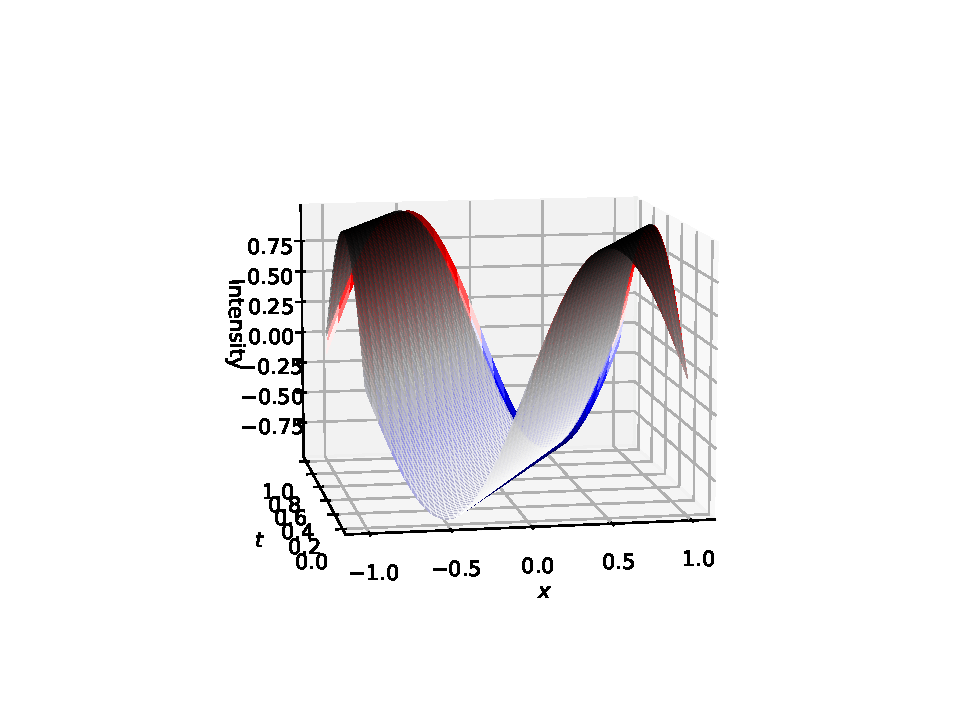
\includegraphics[width=0.85\linewidth]{plots/task4b_numSol.pdf}\label{fig:task4b_numSol}}\hspace{0mm}
\subfloat[Relative error $e^r_{\ell}$]{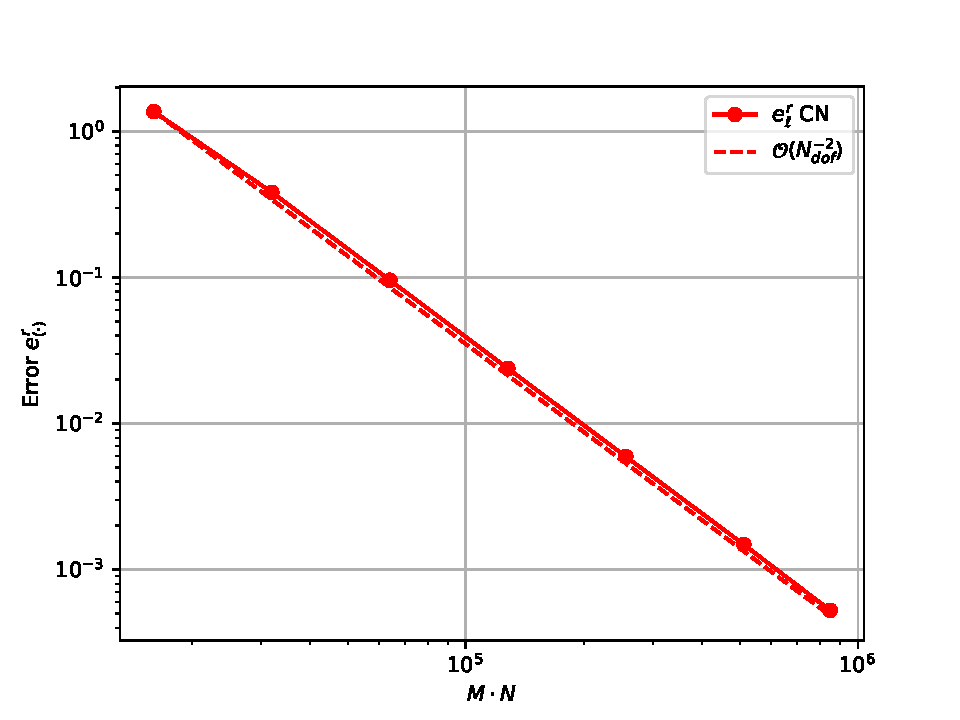
\includegraphics[width=0.85\linewidth]{plots/task4b_error.pdf}\label{fig:task4b_error}}\hspace{0mm}
\caption{Linearized Korteweg-deVries equation on $x \in [-1,1]$ and $t \in [0,1]$, with a periodic boundary condition and initial condition $u(x,0)=\sin{(\pi x)}$. In (a), the analytical solution is shown in grey and the numerical solution is plotted with a \textit{seismic} color map. The numerical solution is calculated using Crank-Nicolson with $M=N=50$. In (b), the relative error $e^r_{\ell}$ at $t=1$ is plotted with the $x$-axis as the number of degrees of freedom. The numerical solution is calculated with Crank-Nicolson where $N=1000$ and $M$ increases exponentially.}
\end{figure}

In order to quantify the convergence of the numerical solution to the analytical solution, the relative error, defined as in equation \eqref{discreteRelativeError}, is calculated. The convergence plot in figure \ref{fig:task4b_error} shows that the discrete $\ell_2$ error goes as $\mathcal{O}(N_{\mathrm{dof}}^{-2})$, as expected, given the truncation error term in \eqref{task4CrankExact}.

\subsubsection{c)}
In this section, a proof of the fact that the continuous $L_2$ norm of the analytical solution in problem \eqref{KdV} is conserved over time, as long as a periodic boundary condition is imposed, will be constructed. The analytical solution can be expressed in a Fourier series on the form

\begin{equation*}
    u(x,t) = \sum_{k \in \mathbb{Z}}\widehat{u}(k,0)\exp{(-i\pi k(1+\pi^2)t + i\pi^3k^3t)}\exp{(i\pi kx)}.
\end{equation*}
Using the notation $u(x,t)^*$ for the complex conjugate of $u(x,t)$, the absolute value of $u(x,t)$ can be expressed with a double summation on the form 

\begin{equation*}
    \begin{split}
        |u(x,t)|^2 &= u(x,t)^* u(x,t) \\ &= \left(\sum_{k \in \mathbb{Z}}\widehat{u}(k,0)^* \mathrm{e}^{i\pi k(1+\pi^2)t - i\pi^3 k^3 t}\mathrm{e}^{-i\pi kx}\right) \left(\sum_{k \in \mathbb{Z}}\widehat{u}(k,0) \mathrm{e}^{-i\pi k(1+\pi^2)t +i\pi^3 k^3t}\mathrm{e}^{i\pi kx}\right) \\ &= \sum_{k\in \mathbb{Z}}\sum_{l \in \mathbb{Z}} \widehat{u}(k,0)^*\widehat{u}(l,0) \mathrm{e}^{i\pi k(1+\pi^2)t-i\pi^3 k^3t}\mathrm{e}^{-i\pi l(1+\pi^2)t+i\pi^3 l^3t }\mathrm{e}^{-i\pi kx}\mathrm{e}^{i\pi lx}.
    \end{split}
\end{equation*}
Integrating over $x \in [-1,1]$ and using the orthogonality of Fourier basis functions, namely that $\int_{-1}^{1} \exp{(-i\pi kx)}\exp{(i\pi lx)} \mathrm{d}x =2\delta_{k,l}$, yields

\begin{equation*}
    \begin{split}
        \int_{-1}^{1} |u(x,t)|^2 \mathrm{d}x &= \sum_{k\in \mathbb{Z}}\sum_{l \in \mathbb{Z}} \widehat{u}(k,0)^*\widehat{u}(l,0) \mathrm{e}^{i\pi k(1+\pi^2)t-i\pi^3 k^3t}\mathrm{e}^{-i\pi l(1+\pi^2)t+i\pi^3 l^3t } \int_{-1}^{1} \mathrm{e}^{-i\pi kx}\mathrm{e}^{i\pi lx} \mathrm{d}x \\ &= 2\sum_{k \in \mathbb{Z}} \widehat{u}(k,0)^*\widehat{u}(k,0) \mathrm{e}^{(i\pi k(1+\pi^2)t-i\pi^3 k^3t)} \mathrm{e}^{-(i\pi k(1+\pi^2)t-i\pi^3 k^3t)} \\ &= 2 \sum_{k \in \mathbb{Z}} \widehat{u}(k,0)^* \widehat{u}(k,0).
    \end{split}
\end{equation*}
In a similar manner, the integral of $|u(x,0)|^2$ can be calculated as 

\begin{equation*}
    \begin{split}
        \int_{-1}^{1} |u(x,0)|^2  &= \sum_{k \in \mathbb{Z}}\sum_{l \in \mathbb{Z}} \widehat{u}(k,0)^*\widehat{u}(l,0) \int_{-1}^{1} \mathrm{e}^{-i\pi kx} \mathrm{e}^{i\pi lx} \mathrm{d}x \\ &= 2\sum_{k \in \mathbb{Z}} \widehat{u}(k,0)^* \widehat{u}(k,0).
    \end{split}
\end{equation*}
Observe that the two integrals are identical to each other. The definition of the $L_2$ norm gives 

\begin{equation*}
\begin{split}
    ||u(x,t)|| &:= \sqrt{\frac{1}{2}\int_{-1}^{1} |u(x,t)|^2\mathrm{d}x} = \sqrt{\frac{1}{2}\int_{-1}^{1} |u(x,0)|^2\mathrm{d}x} \\ &= \sqrt{\sum_{k \in \mathbb{Z}} |\widehat{u}(k,0)|^2}.
\end{split}
\end{equation*}
Hence, the $L_2$ norm is conserved for any time $t > 0$. $\square$

\begin{comment}
One can alternatively show that $\frac{\mathrm{d}}{\mathrm{d}t}|u(x,t)|^2 = 0$. We have 

\begin{equation}
    \frac{\mathrm{d}}{\mathrm{d}t}|u(x,t)|^2 = u_t(x,t)^* u(x, t) + u_t(x, t) u(x, t)^* 
\label{time_der}
\end{equation}

We consider the first term of \eqref{time_der}:

\begin{equation*}
    \begin{split}
        u_t(x,t)^* u(x, t) &= \left(\sum_{k \in \mathbb{Z}}(i\pi k(1 + \pi^2) - i \pi^3 k^3)\widehat{u}(k,t)^* \mathrm{e}^{i\pi k x}\right) \left(\sum_{l \in \mathbb{Z}}\widehat{u}(l,t) \mathrm{e}^{i\pi lx}\right) \\
        &= \sum_{k \in \mathbb{Z}} \sum_{l \in \mathbb{Z}} (i \pi k(1 +\pi^2) - i\pi^3 k^3 ) \mathrm{e}^{i\pi(l - x)} 
    \end{split}
\end{equation*}

\end{comment}

Numerically, the conservation of the $L_2$ norm can be observed by calculating the discrete $\ell_2$ norm and using that as an approximation for the continuous case. By using the discretization method implemented in \textbf{b)}, namely the one based on the Crank-Nicolson method \eqref{task4discCrank}, due to the mentioned stability reasons, the $\ell_2$ norm is calculated as a function of time for two specified initial conditions. The first case is with $u(x,0)=\sin{(\pi x)}$, as in the original problem \eqref{KdV}, and the second case is with $u(x,0)=\sin{(2 \pi x)}$. The plots of the discrete $\ell_2$ norm over time are shown in the figures \ref{fig:task4c_sine} and \ref{fig:task4c_sine_2}. Observe that the $\ell_2$ norm is oscillating around a fixed value and not drifting with time, which is in agreement with the discussion above.

\begin{figure}
\centering
\subfloat[Initial condition $u(x,0)=\sin{(\pi x)}$]{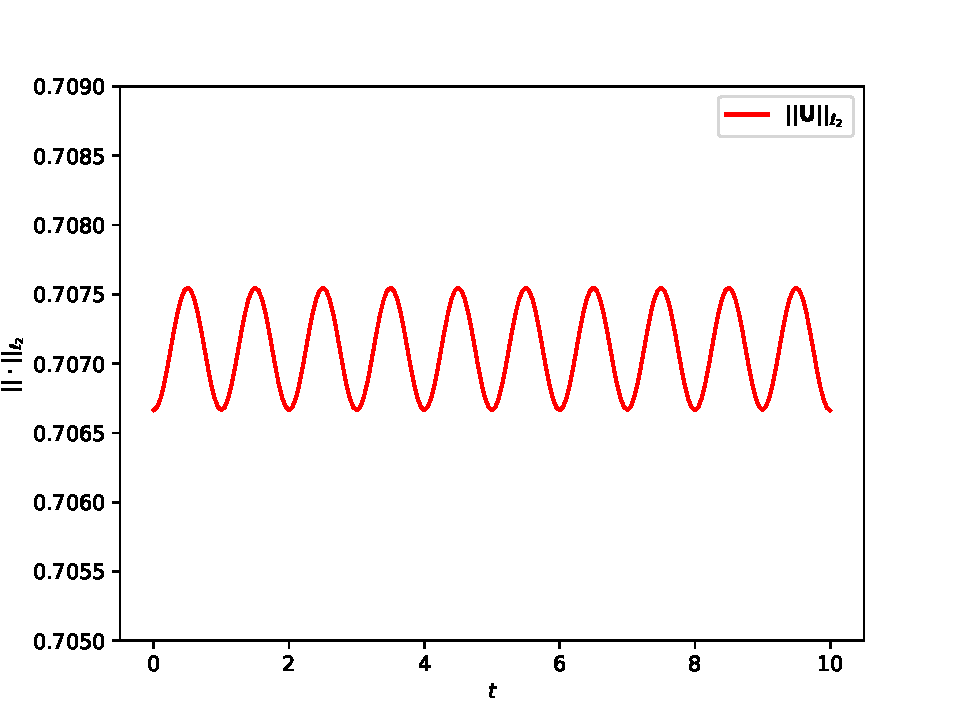
\includegraphics[width=0.85\linewidth]{plots/task4c_sine.pdf}\label{fig:task4c_sine}}\hspace{0mm}
\subfloat[Initial condition $u(x,0)=\sin{(2 \pi x)}$]{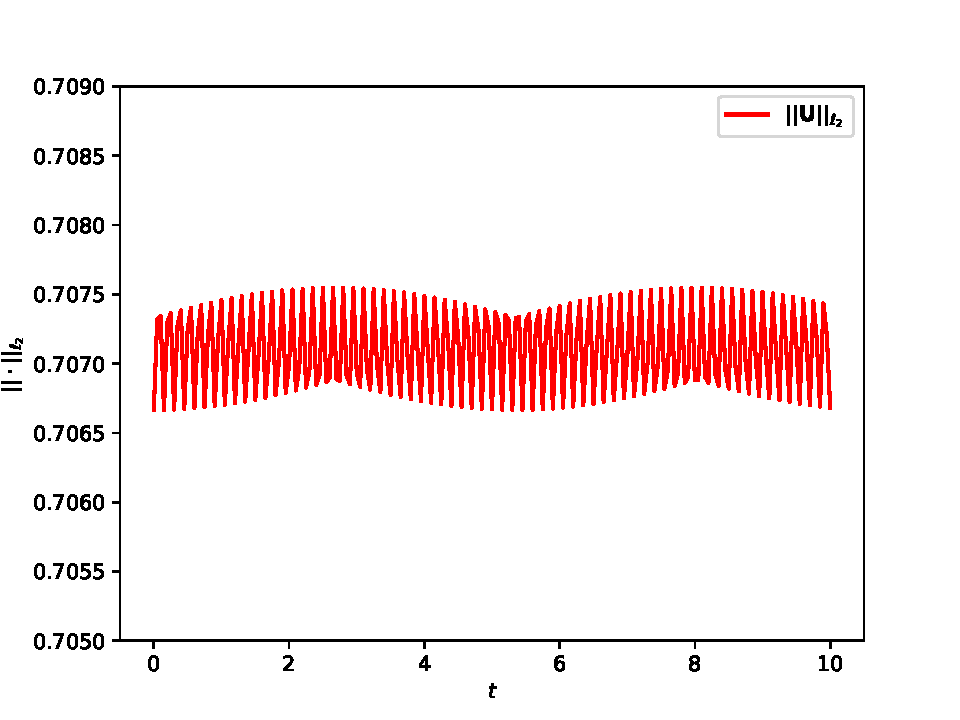
\includegraphics[width=0.85\linewidth]{plots/task4c_sine_2.pdf}\label{fig:task4c_sine_2}}\hspace{0mm}
\caption{Linearized Korteweg-deVries equation on $x \in [-1,1]$ and $t \in [0,10]$, with a periodic boundary condition with period 2. The discrete $\ell_2$ norm of the numerical solution as a function of time, with initial condition $u(x,0)=\sin{(\pi x)}$, is shown in (a) and with initial condition $u(x,0)=\sin{(2 \pi x)}$ in (b). The numerical solution is calculated using the Crank-Nicolson method.}
\end{figure}

\newpage
\ 
\newpage
\newpage

\section{Problem 5 - Poisson Equation in One Dimension}

\subsubsection{a)}

Consider the Poisson equation in 1D

\begin{equation}
\label{task5Poisson}
    -u_{xx} = f(x), \hspace{2mm} u(a) = d_1, \hspace{1mm} u(b) = d_2.
\end{equation}
Assume a uniform partition, i.e. that $x_m = a + mh$, $h = \frac{b-a}{M}$ and $m \in [0,M]$. By discretizing the problem with linear finite elements, a linear system $\mathbf{Au} = \mathbf{f}$ can be created. Since the problem has inhomogeneous Dirichlet boundary conditions, the approach outlined in section 2.5 of \cite{Curry} will be followed, in order to create the system.  
As is done in Curry's note, the inhomogeneous problem will be related to the homogeneous one. The weak form is therefore written with test functions satisfying $v \in H^1_0([a,b])$, i.e. $v(a) = v(b) =0$. The weak form becomes

\begin{align}
    -\int_a^bu''(x)v(x)\mathrm{d}x &= \int_a^bf(x)v(x)\mathrm{d}x, \nonumber \\
    \int_a^bu'(x)v'(x)\mathrm{d}x - [u'(x)v(x)]_a^b &= \int_a^bf(x)v(x)\mathrm{d}x, \nonumber \\
    \int_a^bu'(x)v'(x)\mathrm{d}x &= \int_a^bf(x)v(x)\mathrm{d}x,
    \label{var}
\end{align}

\noindent where $u$ is an element of $H^1([a,b])$. Next, $R_h \in H^1([1,b])$ is introduced, satisfying $R_h(a) = d_1$ and $R_h(b) = d_2$. Then $\hat{u} := u - R_h \in H^1_0([a,b])$ is defined, so the variational \eqref{var} form can be rewritten as 

\begin{equation}
    \int_a^b\hat{u}'(x)v'(x)\mathrm{d}x = \int_a^bf(x)v(x)\mathrm{d}x - \int_a^bR_h'(x) v'(x) \mathrm{d}x.
\label{var2}
\end{equation}

\noindent Using linear finite elements, the functions in \eqref{var2} are now restricted to lie in the finite dimensional subspace $X_h^1$ of $H^1([a,b])$, i.e. the space of piece-wise linear functions with basis $\{\varphi_i\}$ as defined in \cite{Curry}. We partition the grid into $M$ elements, such that $v = \sum_{i = 0}^{M}v_i \varphi_i(x)$ and likewise for $u$ and $\hat{u}$. $R_h$ takes the natural form $R_h = d_1 \varphi_0(x) + d_2 \varphi_M(x)$. Introducing the stiffness matrix $A_{ij} = \int_a^b \varphi'_i(x) \varphi'_j(x) \mathrm{d}x$  such that 

\begin{equation*}
    A =  \frac{1}{h}\begin{pmatrix}
        1 & -1 & 0 & \cdots & \cdots & 0 \\
        -1 & 2 & -1 & \ddots &   & \vdots \\
        0 & -1 & 2 & \ddots & \ddots & \vdots \\
        \vdots & \ddots & \ddots & \ddots & \ddots & 0 \\
        \vdots &  & \ddots & -1 & 2 & -1 \\
        0 & \cdots & \cdots & 0 & -1 & 1
    \end{pmatrix} \in \mathbb{R}^{(M+1) \times (M+1)},
\end{equation*}

\noindent and removing $v$, the equation \eqref{var2} becomes

\begin{equation}
\begin{split}
    A\hat{u} &= F-A(d_1, 0, \dots, 0, d_2)^T \\
             &= 
            \frac{1}{h}\begin{pmatrix}
                Q_0[(x_1 - x) f(x)] \\
                Q_0[(x - x_0) f(x)] + Q_1[(x_2 - x) f(x)] \\
                \vdots \\
                Q_{M-2}[(x - x_{M-2}) f(x)] + Q_{M-1}[(x_M - x) f(x)] \\
                Q_{M-1}[(x - x_{M-1}) f(x)]
            \end{pmatrix}
            -
            \frac{1}{h} \begin{pmatrix}
                d_1 \\
                -d_1 \\
                \vdots \\
                -d_2 \\
                d_2
            \end{pmatrix},
\label{task5system}
\end{split}
\end{equation}
where $Q_k[g(x)]$ denotes the Gaussian quadrature of the function $g$ over the interval $[x_k, x_{k + 1}]$. In the numerical implementation, we have use Gauss-Legendre quadrature with 5 sample points and weights. Then, the boundary conditions are implemented by removing the first and last row and column from the stiffness matrix $A$ on the left side of equation \eqref{task5system}, in addition to the first and last entries of the vector $F - A(d_1, \ldots, d_2)^T$. The resulting matrix and vector are given as

\begin{equation}
\begin{split}
    &\mathbf{A} :=  \frac{1}{h}\begin{pmatrix}
        -2 & -1 &  &  \\
        -1 & \ddots & \ddots &  \\
         & \ddots & \ddots & -1  \\
         &  & -1 & 2  \\
    \end{pmatrix} \in \mathbb{R}^{(M-1) \times (M-1)}, \\  \\
     &\mathbf{f} := 
    \begin{pmatrix}
                Q_0[(x - x_0) f(x)] + Q_1[(x_2 - x) f(x)]  + d_1/h\\
                \vdots \\
                Q_{M-2}[(x - x_{M-2}) f(x)] + Q_{M-1}[(x_M - x) f(x)] + d_2/h 
    \end{pmatrix} \in \mathbb{R}^{(M-1) \times 1},
\end{split}
\label{5a.system}
\end{equation}
respectively. Also, define $\mathbf{u} := \hat{u}$, so the system to be solved can be written as $\mathbf{Au} = \mathbf{f}$. Finally, when this system is solved, the vector $\hat{u}$ is expanded from dimension $M-1$ to $M+1$ by including $d_1$ as first entry and $d_2$ as the last, i.e. take $u(x) = \hat{u}(x) + R_h(x)$. 


\subsubsection{b)}
Now consider $0 \le x \le 1$ with 

\begin{equation}
    f(x) = -2, \quad d_1 = 0, \; d_2 = 1.
\label{5b}
\end{equation}
First, the analytical solution is calculated. The Poisson equation reads $-u_{xx} = -2$, which yields

\begin{equation}
    u(x) = x^2 + c_1x + c_2,
\end{equation}
where $c_1,c_2 \in \mathbb{R}$ are constants. The boundary conditions finally give $c_1 = c_2 = 0$, resulting in

\begin{equation}
    u(x) = x^2.
\end{equation}

When using the finite element method, both uniform mesh refinement (hereafter UFEM) and adaptive mesh refinement (hereafter AFEM) is performed. In the rest of the problem, when performing UFEM, $M = \{8,16,32,64,128,256,512,1024,2048\}$ will be used. On the contrary, AFEM will be performed using \textit{average}-error with $\alpha = 1$, and \textit{max}-error with $\alpha = 0.7$ as it is defined in section \ref{adaptive}.

Convergence plots, where the difference between analytical and numerical solution in $L_2$-norm is calculated, for both UFEM and AFEM are depicted in figure \ref{fig:5b}. It is apparent that all methods converge with order $\mathcal{O}(h^2)$ in $L_2$ norm. It can be shown that this is the expected theoretical result \cite{Curry}.

\begin{figure}[!t]
  \centering
  \subfloat[]{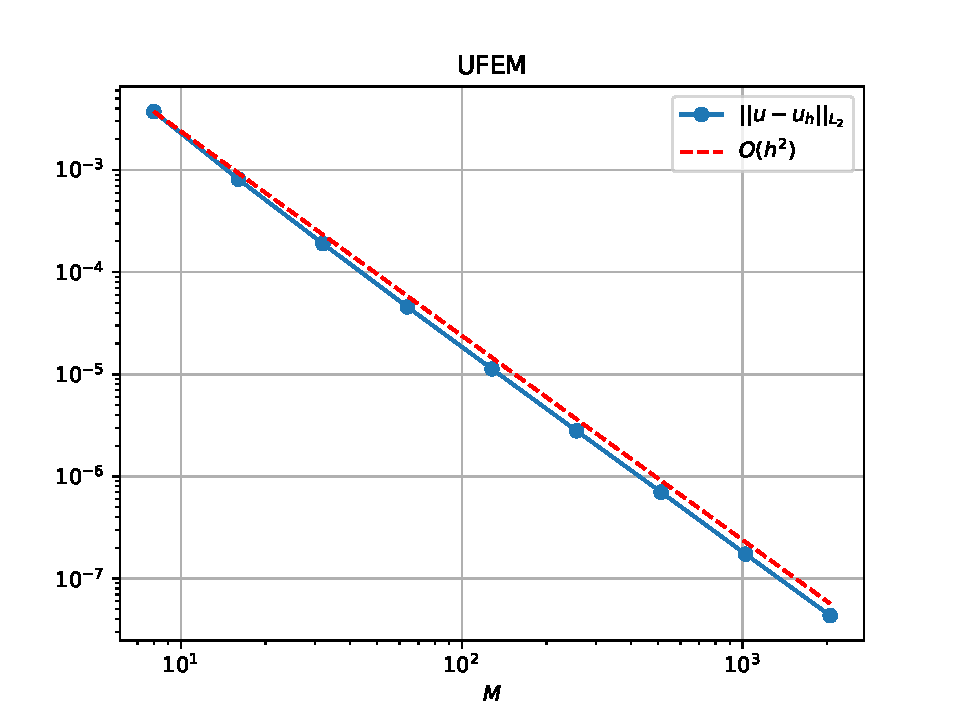
\includegraphics[width=0.5\textwidth]{plots/5b_UFEM.pdf}\label{fig:f1}}
  \hfill
  \subfloat[]{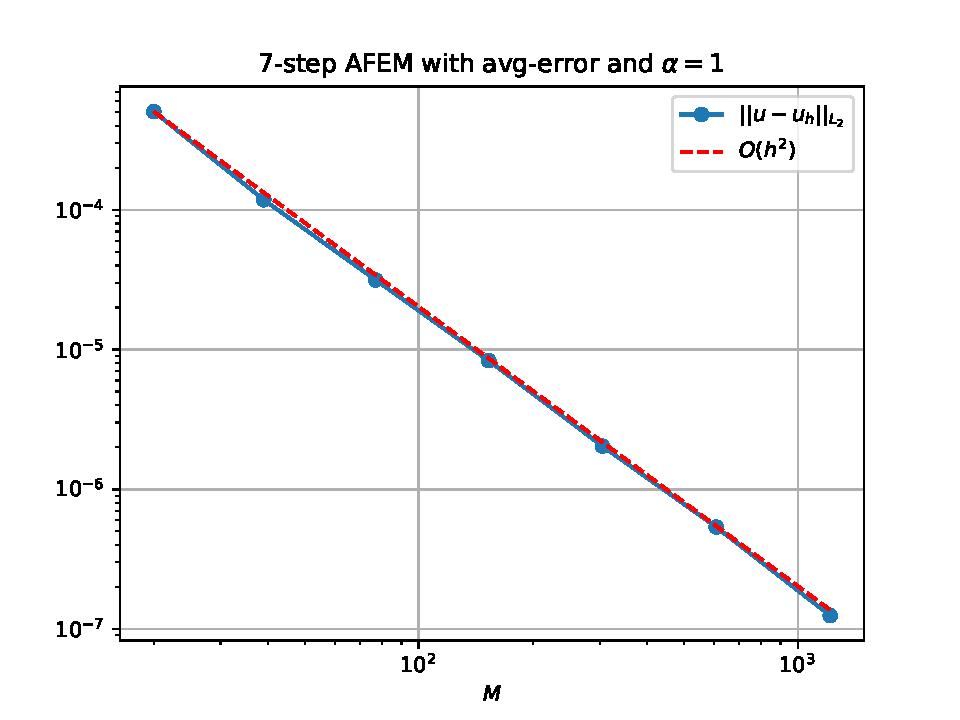
\includegraphics[width=0.5\textwidth]{plots/5b_avgAFEM.pdf}\label{fig:f2}}
  \hfill
  \subfloat[]{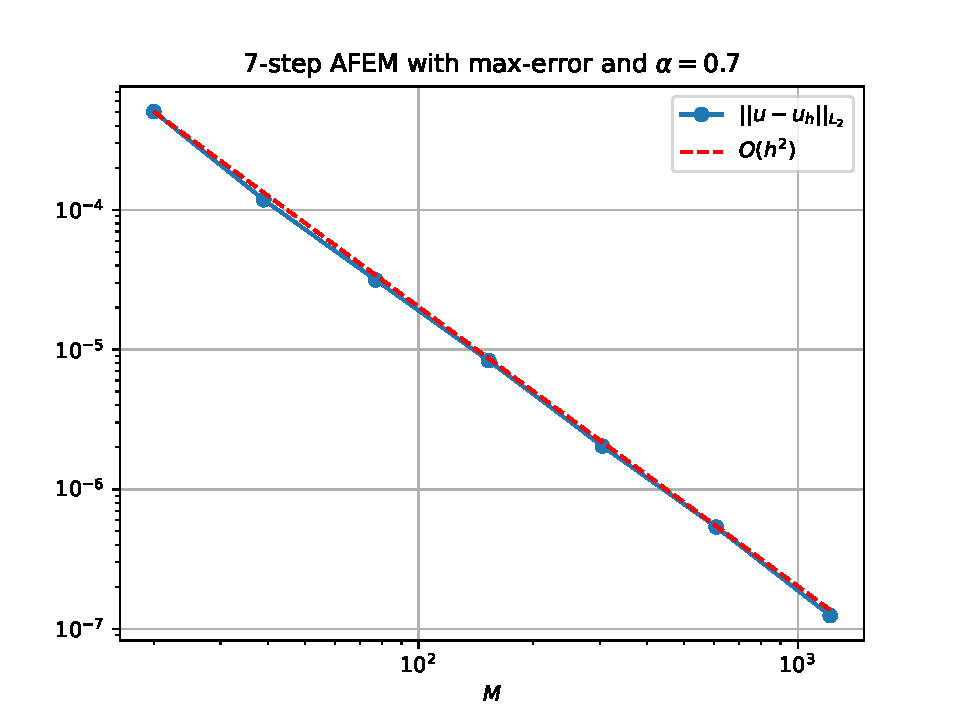
\includegraphics[width=0.5\textwidth]{plots/5b_maxAFEM.pdf}\label{fig:f3}}
  \caption{One dimensional Poisson equation $-u_{xx} = -2$ with $x \in [0,1]$ and $u(0) = 0, u(1) = 1$. The $L^2$-error is displayed in "log-log" plots. $u_h$ is the numerical solution while $u$ is the analytical solution. (a) UFEM. (b) AFEM with average-error and $\alpha = 1$. (c) AFEM with maximum-error and $\alpha = 0.7$.}
  \label{fig:5b}
\end{figure}

\subsubsection{c)}
Next, consider $-1 \le x \le 1$ with 

\begin{equation}
    f(x) = -(40000x^2-200)e^{-100x^2}, \quad d_1 = e^{-100}, \; d_2 = e^{-100}.
\label{5c}
\end{equation}
First, the analytical solution is calculated. The Poisson equation reads

\begin{equation}
    u_{xx} =  200e^{-100x^2} - 40000x^2 \cdot e^{-100x^2},
\end{equation}
which gives

\begin{equation}
    u(x) = e^{-100x^2} + c_1x + c_2
\end{equation}
The boundary conditions readily give that $c_1 = c_2 = 0$, which means the analytical solution is

\begin{equation}
u(x) = e^{-100x^2}.
\end{equation}

\noindent The convergence plots for UFEM and AFEM, in this case, are depicted in figure \ref{fig:5c}. It is apparent that all methods converge with order $\mathcal{O}(h^2)$ in $L_2$ norm.

\begin{figure}[!t]
  \centering
  \subfloat[]{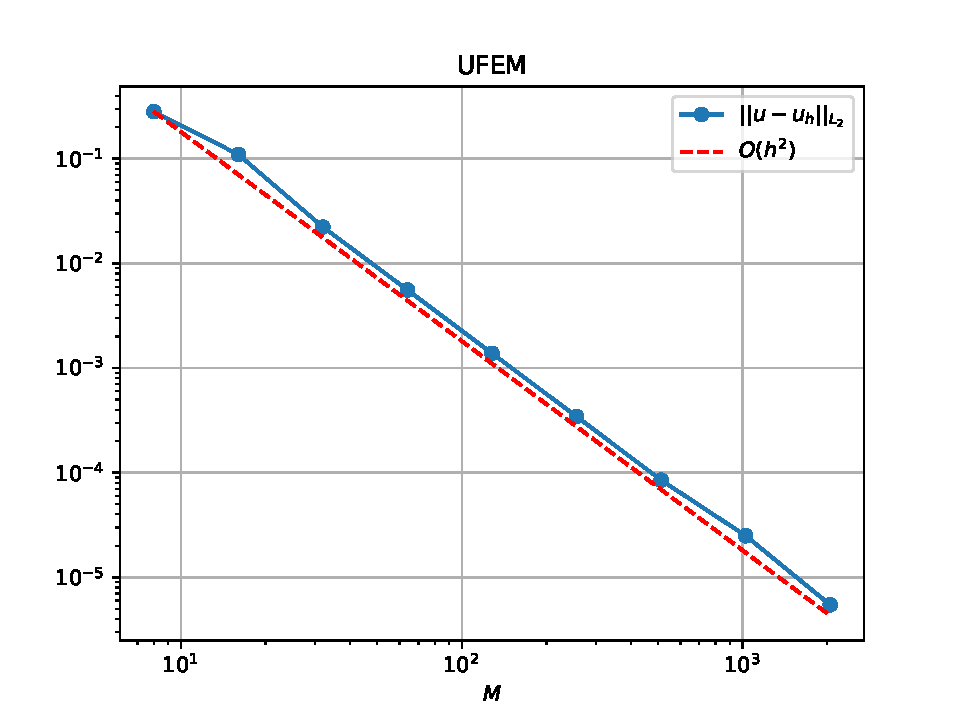
\includegraphics[width=0.5\textwidth]{plots/5c_UFEM.pdf}\label{fig:f1}}
  \hfill
  \subfloat[]{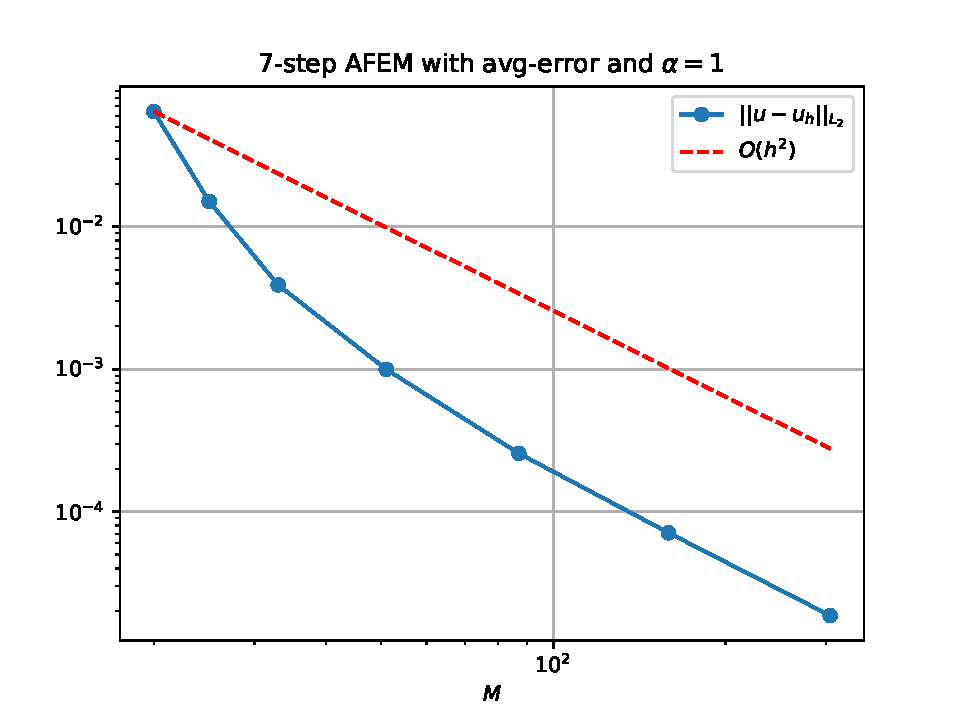
\includegraphics[width=0.5\textwidth]{plots/5c_avgAFEM.pdf}\label{fig:f2}}
  \hfill
  \subfloat[]{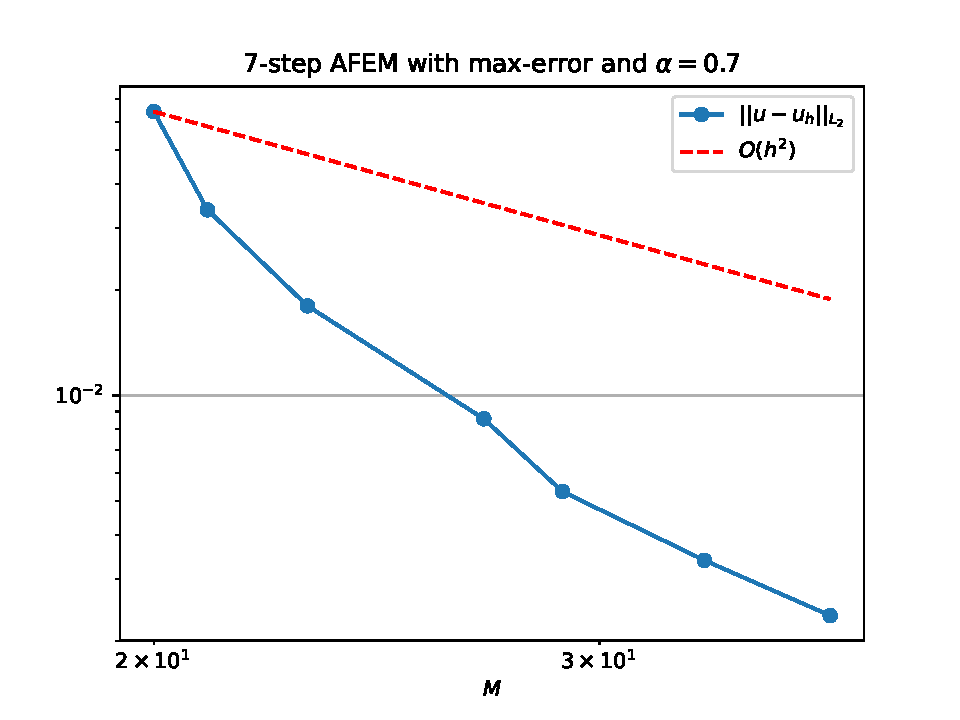
\includegraphics[width=0.5\textwidth]{plots/5c_maxAFEM.pdf}\label{fig:f3}}
  \caption{One dimensional Poisson equation $-u_{xx} = -(40000x^2 - 200)e^{-100x^2}$ with $x \in [-1,1]$ and $u(-1) = u(1) = e^{-100}$. The $L^2$-error is displayed in "log-log" plots. $u_h$ is the numerical solution while $u$ is the analytical solution. (a) UFEM. (b) AFEM with average and $\alpha = 1$. (c) AFEM with maximum and $\alpha = 0.7$.}
  \label{fig:5c}
\end{figure}

\subsubsection{d)}

Now consider $-1 \le x \le 1$ with

\begin{equation}
    f(x) = -(4000000x^2 - 2000)e^{-1000x^2}, \quad d_1 = e^{-1000}, \; d_2 = e^{-1000}.
\label{5d}
\end{equation}
\noindent The derivation of the analytical solution is entirely analogous the one in c). Thus,

\begin{equation}
    u(x) = e^{-1000x^2}.
\end{equation}

\noindent The convergence plots for UFEM and AFEM are depicted in figure \ref{fig:5d}. It is apparent that all methods converge with order of at least $\mathcal{O}(h^2)$ in $L_2$ norm.

\begin{figure}[!t]
  \centering
  \subfloat[]{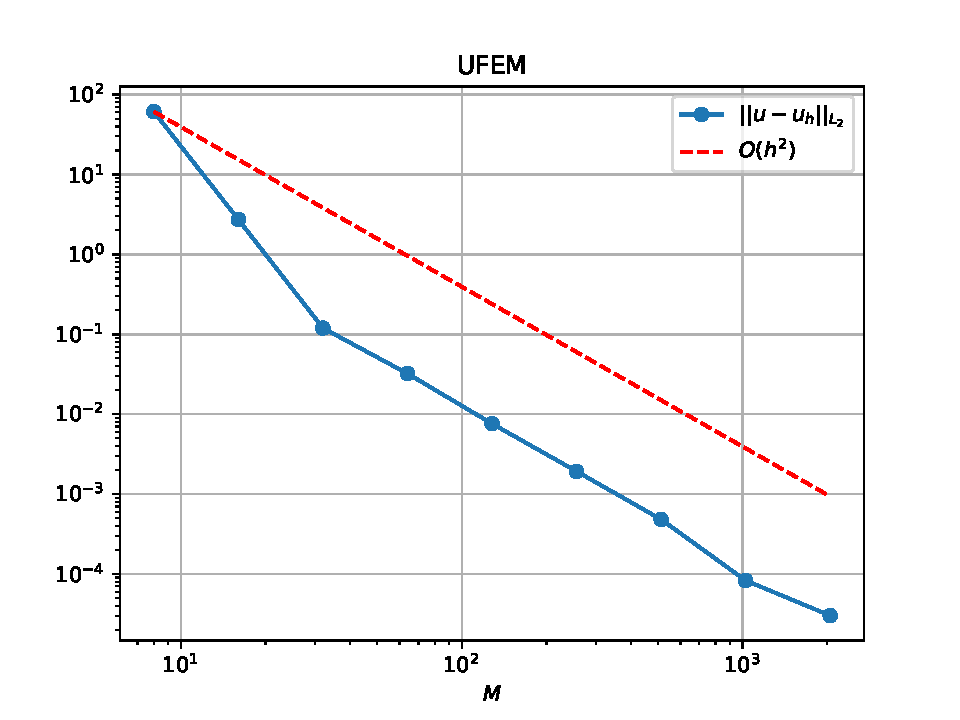
\includegraphics[width=0.5\textwidth]{plots/5d_UFEM.pdf}\label{fig:f1}}
  \hfill
  \subfloat[]{\includegraphics[width=0.5\textwidth]{plots/5d_avgAFEM.pdf}\label{fig:f2}}
  \hfill
  \subfloat[]{\includegraphics[width=0.5\textwidth]{plots/5d_maxAFEM.pdf}\label{fig:f3}}
  \caption{One dimensional Poisson equation $-u_{xx} = -(4000000x^2 - 2000)e^{-1000x^2}$ with $x \in [-1,1]$ and $u(-1) = u(1) = e^{-1000}$. The $L^2$-error is displayed in "log-log" plots. $u_h$ is the numerical solution while $u$ is the analytical solution. (a) UFEM. (b) AFEM with average and $\alpha = 1$. (c) AFEM with maximum and $\alpha = 0.7$.}
  \label{fig:5d}
\end{figure}

\subsubsection{e)}
Finally, consider $0 \le x \le 1$, with

\begin{equation}
    f(x) = \frac{2}{9}x^{-4/3}, \quad d_1 = 0, \; d_2 = 1
\label{5e}
\end{equation}
Integraiton yields that $u$ must be on the form $u(x) = x^{2/3} + c_1x + c_2$, where $c_1,c_2 \in \mathbb{R}$ are constants. The boundary conditions give $c_1 = 0$ and  $c_2 = 0$, so we arrive at the analytical solution

\begin{equation}
    u(x) = x^{2/3}.
\end{equation}

\noindent The convergence plots for UFEM and AFEM are depicted in figure \ref{fig:5e}. We observe that using uniform refinement only yields a convergence of order $\mathcal{O}(h)$ in this case. One possible explanation for this is that the analytical solution, $u(x)$ is not sufficiently smooth. For example, it is assumed that the variational, written as

\begin{equation}
    \int_0^1 u'(x) v'(x) \mathrm{d}x= \int_0^1 f(x)v(x) \mathrm{d}x
\label{varform}
\end{equation}

\noindent should hold for all $v \in H_0^1([0,1])$, where $v(0) = v(1) = 0$. If we let $v(x) = \sin(\pi x)$, the left hand side of \eqref{varform} becomes

\begin{equation}
\begin{split}
    \int_0^1 f(x)v(x) \mathrm{d}x &= \int_0^1 \frac{2}{9}x^{-\frac{4}{3}} \cdot \sin(\pi x) \mathrm{d}x \\
    &= \left[\frac{2}{9}x^{-\frac{4}{3}} \cdot (-\frac{1}{\pi}\cos(\pi x))\right]_0^1 - \int_0^1  \frac{8}{27} x^{-\frac{7}{3}} \cdot \frac{1}{\pi}\cos(\pi x) \mathrm{d}x,
\end{split}
\end{equation}

\noindent where it is readily seen that the first term is not defined for $x = 0$. The AFEM method with average error also seems to have a lower convergence rate compared to the other examples, while AFEM with max-error seems to uphold the convergence of rate $\mathcal{O}(h^2)$.

\begin{figure}[!t]
  \centering
  \subfloat[]{\includegraphics[width=0.5\textwidth]{plots/5e_UFEM.pdf}\label{fig:f1}}
  \hfill
  \subfloat[]{\includegraphics[width=0.5\textwidth]{plots/5e_avgAFEM.pdf}\label{fig:f2}}
  \hfill
  \subfloat[]{\includegraphics[width=0.5\textwidth]{plots/5e_maxAFEM.pdf}\label{fig:f3}}
  \caption{One dimensional Poisson equation $-u_{xx} = -\frac{2}{9}x^{-4/3}$ with $x \in [0,1]$ and $u(0) = 0,  u(1) = 1$. The $L^2$-error is displayed in "log-log" plots. $u_h$ is the numerical solution while $u$ is the analytical solution. (a) UFEM. (b) AFEM with average and $\alpha = 1$. (c) AFEM with maximum and $\alpha = 0.7$.}
  \label{fig:5e}
\end{figure}
\newpage
\ 
\newpage

\newpage


\chapter{Part 2}
\section{Problem 2 - Sine-Gordon Equation}
\label{"part 2"}
Consider the Sine-Gordon equation on $\Omega \times I$, where $\Omega = [a,b]$ and $I = [0, T]$

\begin{align}
    &u_{tt} - u_{xx} + \sin{(u)} = 0, &&(x,t) \in \Omega \times I, \label{sine-gordon} \\
    &u(a,t) = f_1(t), \hspace{1mm} u(b,t) = f_2(t),  &&(x,t) \in \partial\Omega \times I,\label{sine-gordon-BC} \\
    &u(x,0) = u_0(x), \hspace{1mm} u_t(x,0) = u_1(x), &&x \in \Omega \times \{t=0\}. \label{sine-gordon-IC}
\end{align}

\subsubsection*{a)}

The analytical solution will be derived in the following. By introducing the change of variables $s = x - ct$, the equation \eqref{sine-gordon} can be expressed differently, because

\begin{equation*}
\begin{split}
    \frac{\partial u}{\partial t} &= \frac{\partial u}{\partial s}\frac{\partial s}{\partial t} = -c\frac{\partial u}{\partial s}, \\
    \frac{\partial^2 u}{\partial t^2} &= \frac{\partial }{\partial t}\left(-c\frac{\partial u}{\partial s}\right) = -c \frac{\partial }{\partial s}\frac{\partial u}{\partial t} = c^2 \frac{\partial^2 u}{\partial s^2}, \\
    \frac{\partial u}{\partial x} &= \frac{\partial u}{\partial s}\frac{\partial s}{\partial x} = \frac{\partial u}{\partial s}, \\
    \frac{\partial^2 u}{\partial x^2} &= \frac{\partial }{\partial x}\frac{\partial u}{\partial s} = \frac{\partial }{\partial s}\frac{\partial u}{\partial x} = \frac{\partial^2 u}{\partial s^2}. \\
\end{split}
\end{equation*}
This leads to the Sine-Gordon equation \eqref{sine-gordon} on the following form

\begin{equation*}
    \left(1-c^2\right)u_{ss} = \sin{(u)}.
\end{equation*}
Multiplying the equation by $u_s$ and performing integration by parts yields

\begin{align*}
    (1-c^2)\int u_{ss}u_s\mathrm{d}s &= (1-c^2)\left((u_{s})^2 - \int u_{ss}u_s\mathrm{d}s \right) + D_1\nonumber \\
    \implies (1-c^2)\int u_{ss}u_s\mathrm{d}s &= (1-c^2)\frac{1}{2}(u_{s})^2 + D_2, 
\end{align*}

where $D_2 = \frac{1}{2}D_1$, for the left hand side and 

\begin{equation*}
     \int \sin{(u)}u_s \mathrm{d}s = -\cos{(u)} + D_3,
\end{equation*}
for the right hand side. Hence, 

\begin{equation*}
    \frac{1}{2}(1-c^2)u^2_s = -\cos{(u)} + D, 
\end{equation*}
where $D = D_3 - D_2$. The constant $D$ determines one unique solution to the problem. Let $D = 1$ in this case. Thus, note that 

\begin{align*}
    u^2_s &= \frac{2(1 - \cos{(u)})}{(1-c^2)} \nonumber \\
    u^2_s &= \frac{4\sin^2{(\frac{u}{2})}}{(1-c^2)} \nonumber \\
    \frac{u_s}{\sin{(\frac{u}{2})}} &= \pm \frac{2}{\sqrt{1-c^2}}, 
\end{align*}
which, by integrating again, yields 

\begin{align*}
    &\frac{\mathrm{d}u}{\sin{(\frac{u}{2})}} = \pm \frac{2}{\sqrt{1-c^2}} \mathrm{d}s \nonumber \\
    &\mathrm{ln}\tan{\frac{u}{4}} = \pm \frac{s}{\sqrt{1-c^2}} + C \nonumber \\
    u(s) &= 4\arctan{\left(\exp{\left\{\pm \frac{s}{\sqrt{1-c^2}}\right\}}\right)},
\end{align*}
where the integration constant $C$ is set to 0. This means that one possible analytical solution to the Sine-Gordon equation \eqref{sine-gordon} is 

\begin{equation}
    u(x,t) = 4\arctan{\left(\exp{\left\{\pm \frac{x-ct}{\sqrt{1-c^2}}\right\}}\right)}, 
    \label{Part2-analytic-solution}
\end{equation}
when the integration constants are set to 0 and 1. 

\subsubsection*{b)} 
The following statement is proved in this section.
\begin{mydef}
The energy is conserved when $u_x(a,t) = u_x(b,t) = 0$.
\end{mydef}
\begin{proof}
The energy is the quantity that is obtained after multiplying equation \eqref{sine-gordon} by $u_t$ and integrating with respect to both $x$ and $t$. Before integrating, note the following equivalence relation

\begin{equation}
\begin{split}
    &u_tu_{tt} - u_tu_{xx} + u_t\sin{(u)} = 0 \\
    \iff &\frac{\partial}{\partial t}\left(\frac{1}{2}\left(\frac{\partial u}{\partial t}\right)^2 + \frac{1}{2}\left(\frac{\partial u}{\partial x}\right)^2 - \cos{(u)}\right) - \frac{\partial }{\partial x}\left(\frac{\partial u}{\partial t}\frac{\partial u}{\partial x}\right) = 0.
\label{part2b}
\end{split}
\end{equation}
This can be verified by noting that

\begin{equation*}
\begin{split}
    \frac{\partial}{\partial t}\left(\frac{1}{2}\left(\frac{\partial u}{\partial t}\right)^2 + \frac{1}{2}\left(\frac{\partial u}{\partial x}\right)^2 - \cos{(u)}\right) - \frac{\partial }{\partial x}\left(\frac{\partial u}{\partial t}\frac{\partial u}{\partial x}\right) &= 0, \\
    \frac{\partial^2 u}{\partial t^2}\frac{\partial u}{\partial t} + \frac{\partial^2 u}{\partial t \partial x}\frac{\partial u}{\partial x} + \frac{\partial u}{\partial t}\sin{(u)} - \left(\frac{\partial u}{\partial t}\frac{\partial^2 u}{\partial x^2} + \frac{\partial u}{\partial x}\frac{\partial^2 u}{\partial t\partial x}\right) &= 0.
\end{split}
\end{equation*}
Hence, integration of \eqref{part2b} yields

\begin{align}
    0 &=\int_0^{t'}\int_a^b\left(u_tu_{tt} - u_tu_{xx} + u_t\sin{(u)}\right)\mathrm{d}x\mathrm{d}t\nonumber \\
    &=\int_0^{t'} \int_a^b\left\{\frac{\partial}{\partial t}\left(\frac{1}{2}\left(\frac{\partial u}{\partial t}\right)^2 + \frac{1}{2}\left(\frac{\partial u}{\partial x}\right)^2 - \cos{(u)}\right) - \frac{\partial }{\partial x}\left(\frac{\partial u}{\partial t}\frac{\partial u}{\partial x}\right)\right\} \mathrm{d}x\mathrm{d}t, \nonumber \\
    &=\int_0^{t'}\int_a^b \frac{\partial}{\partial t}\left(\frac{1}{2}\left(\frac{\partial u}{\partial t}\right)^2 + \frac{1}{2}\left(\frac{\partial u}{\partial x}\right)^2 - \cos{(u)}\right)\mathrm{d}x\mathrm{d}t - \int_0^{t'}\int_a^b\frac{\partial }{\partial x}\left(\frac{\partial u}{\partial t}\frac{\partial u}{\partial x}\right)\mathrm{d}x\mathrm{d}t.
    \label{energyDoubleIntegration}
\end{align}
Note that

\begin{equation*}
    \int_a^b\frac{\partial }{\partial x}\left(\frac{\partial u}{\partial t}\frac{\partial u}{\partial x}\right)\mathrm{d}x = u_t(b,t^*)u_x(b,t^*)-u_t(a,t^*)u_x(a,t^*) = 0, 
\end{equation*}
when $u_x(b,t^*) = u_x(a,t^*) = 0, \hspace{1mm} \forall t^* \in I$ holds. This means that the second integral in equation \eqref{energyDoubleIntegration} evaluates to zero. Hence, the first integral must also evaluate to zero, which yields

\begin{equation*}
    \begin{split}
        0 &= \int_0^{t'}\int_a^b \frac{\partial}{\partial t} \left(\frac{1}{2}u_t^2 + \frac{1}{2}u_x^2 - \cos{(u)}\right)  \mathrm{d}x\mathrm{d}t \\
        &= \oint_\mathcal{C} \left(-\frac{1}{2}u_t^2 - \frac{1}{2}u_x^2 + \cos{(u)}\right)\mathrm{d}x \quad \text{(Green's Theorem)} \\
        &= -\left[ \int_a^b \left(-\frac{1}{2}u_t^2 - \frac{1}{2}u_x^2 + \cos{(u)}\right)\mathrm{d}x\right]_{t = t'} +  \left[ \int_a^b \left(-\frac{1}{2}u_t^2 - \frac{1}{2}u_x^2 + \cos{(u)}\right)\mathrm{d}x\right]_{t = 0} \\
        &= \left[ \int_a^b E_x\mathrm{d}x\right]_{t = t'} - \left[ \int_a^b E_x\mathrm{d}x\right]_{t = 0} \\
        &= E(t') - E(0), 
    \end{split}
\end{equation*}
where $E_x(x,t) := \frac{1}{2}u_t^2 + \frac{1}{2}u_x^2 - \cos{(u)}$, $E(t') := \left[ \int_a^b E_x\mathrm{d}x\right]_{t = t'}$ and $\mathcal{C}$ is the positively (anticlockwise) oriented boundary of the region $\{(x,t) \hspace{1mm} | \hspace{1mm} a \leq x \leq b, 0 \leq t \leq t' \}$. This shows that the energy $E$ is conserved, since $E(t') = E(0)$. 
\end{proof}

In the literature, e.g. \cite{SG-energy}, the energy density is usually defined as $E_x(x,t) = \frac{1}{2}u_t^2 + \frac{1}{2}u_x^2 + 1 - \cos{(u)}$. This does not contradict our derivation, because an arbitrary constant could have been included inside the parenthesis in the equivalence relation \eqref{part2b}. Therefore, this convention will be used in the following, in order to ensure that the energy is a positive quantity. 

\begin{comment}
% Siste linje du hadde ovenfor, Jim, i tilfelle du vil ha den.
&= \left[-\frac{1}{2}(\|u_t\|^2_{L_2} + \|u_x\|^2_{L_2}) + \int_a^b \cos{u} \mathrm{d}x\right]_{t = t}  + \left[-\frac{1}{2}(\|u_t\|^2_{L_2} + \|u_x\|^2_{L_2}) + \int_b^a \cos{u} \mathrm{d}x\right]_{t = 0}
\end{comment}

\begin{comment}
\textcolor{blue}{Jostein sitt forslag til hva som kan stemme; Jeg tror ikke energien er hele likningen integrert for da hadde den vært null hele tiden.}

From the equation above \eqref{energyDoubleIntegration} we find that
\begin{equation}
\begin{split}
    0 &= \frac{\mathrm{d}}{\mathrm{d}t} \int_0^t \int_a^b \left(\frac{1}{2}u_t^2 + \frac{1}{2}u_x^2 - \cos{u}\right)  \mathrm{d}x\mathrm{d}t = \frac{\mathrm{d}}{\mathrm{d}t} E(t),
\end{split}
\end{equation}
and hence the energy is a constant equal to its initial energy $E(t) = E(0)$. \textcolor{red}{Er nettopp dette jeg har prøvd å vise også :) Hvordan vet du at $E(t)$ er hele dette integralet?} \textcolor{green}{Jim: Står det ikke noe på piazza om at man skal komme fram til et uttrykk uten integraltegn?} \textcolor{blue}{Jo, det står, men vi vet jo fortsatt ikke hvordan E(t) er definert, så det hjelper jo ikke så veldig mye...}
\end{comment}

\subsubsection*{c)}
The Sine-Gordon equation \eqref{sine-gordon} is discretized using the principle of semi-discretization \cite{Owren}. Two systems of ODEs are developed; one with first order and one with second order in time.

\begin{comment}
To begin with, the domain $\Omega \times I$ is discretized along the $x$- and $t$-directions in the following way
\begin{equation*}
\begin{split}
    &x_0 = a \text{,} \hspace{2mm} x_1 = a+\frac{b-a}{M+1} \text{,} \hspace{2mm} \dots \text{,} \hspace{2mm} x_M = a+\frac{M(b-a)}{M+1} \text{,} \hspace{2mm} x_{M+1} = b, \\
    &t_0 = 0 \text{,} \hspace{2mm} t_1 = \frac{T}{N} \text{,} \hspace{2mm} \dots \text{,} \hspace{2mm} t_{N-1} = \frac{T(N-1)}{N} \text{,} \hspace{2mm} t_{N} =T.
\end{split}
\end{equation*}
Let $h = \frac{b-a}{M+1}$ and $k=\frac{T}{N}$.
\end{comment}
To begin with, the $x$-axis is discretized in the following manner

\begin{equation*}
    x_0 = a \text{,} \hspace{2mm} x_1 = a+\frac{b-a}{M+1}, \ldots , x_M = a+\frac{M(b-a)}{M+1},  x_{M+1} = b,
\end{equation*}
letting $h = \frac{b-a}{M+1}$.
A central finite difference approximation is used to discretize the spatial derivative. Let $u_m := u(x_m, t)$. The stencil is then on the form 

\begin{equation*}
    (u_m)_{xx} = \frac{1}{h^2} \delta^2 u_m = \frac{1}{h^2}(u_{m-1} - 2u_m + u_{m+1}) + \mathcal{O}(h^2), \quad 1 \le m \le M, 
\end{equation*}
%where $x_m=a+m h$ and $t_n=n k$ are on the grid defined earlier. 
\noindent Inserting the stencil for the spatial derivative into the Sine-Gordon equation \eqref{sine-gordon} gives

\begin{equation*}
    \ddot{u}_m = \frac{1}{h^2}\delta^2u_m - \sin{(u_m)} + \mathcal{O}(h^2),
\end{equation*}
where the quantity $\ddot{u}_m$ denotes the second order derivative of $u_m$ with respect to time. Note that this is a set of ordinary differential equations (ODE) along lines parallel to the $t$-axis and across the $x$-axis at the grid points $x_m$. Next, the approximate solutions $v_m := v_m(t) \approx u_m(t)$ are introduced, where the truncation error is neglected, by requiring that 

\begin{equation*}
    \ddot{v}_m = \frac{1}{h^2}\delta^2 v_m - \sin{(v_m)} \text{,} \hspace{2mm} 1 \le m \le M.
\end{equation*} 
Considering the Dirichlet boundary conditions \eqref{sine-gordon-BC}, namely that $u(a,t) = v_0(t) = f_1(t)$ and $u(b,t)=v_{M+1}(t)= f_2(t)$, the ODEs can be reformulated in the following manner

\begin{equation}
    \boldsymbol{\ddot{v}} = \frac{1}{h^2} 
    \begin{pmatrix}
    -2 & 1 & 0 & \dots & 0\\
    1 & -2 & 1 & 0 & \dots \\
    \ddots & \ddots & \ddots & \ddots &\ddots \\
    0 & \dots & 1 & -2 & 1 \\
    0 & \dots & 0 & 1 & -2 \\
    \end{pmatrix}
    \boldsymbol{v} + 
    \begin{pmatrix}
    \frac{1}{h^2} f_1(t) - \sin{(v_1)} \\
    -\sin{(v_2)} \\
    \vdots \\
    -\sin{(v_{M-1})} \\
    \frac{1}{h^2} f_2(t) - \sin{(v_M)}\\
    \end{pmatrix} %\text{,} \hspace{2mm} 0 \leq n \leq N
    \label{part2cFirstSystem}
\end{equation}

\noindent where $\boldsymbol{v} = [v_1,v_2,\dots,v_M]^T$ and $\boldsymbol{\ddot{v}} = [\ddot{v}_1,\ddot{v}_2,\dots,\ddot{v}_M]^T$. In compact notation, the system of equations \eqref{part2cFirstSystem} can be written as

\begin{comment}
Note that the boundary functions are evaluated in continuous time, and not with $t=t_n$ on the grid defined earlier. This is because, later, when using ODE-solvers defined below, the system can be dependent of time and this proves therefore to be more accurate \textcolor{red}{Dobbelsjekke dette. Utdype kanskje?} \textcolor{blue}{Ja, det kan være en idé. Ikke helt sikker på hva dette betyr akk nå, men det blir kanskje klarere jo lenger jeg leser :) t-aksen blir jo diskretisert når metodene brukes i praksis uansett?}. 
\end{comment}

\begin{equation}
    \label{SG-disc_2nd_order_in_time}
    \boldsymbol{\ddot{v}} = \frac{1}{h^2}A\boldsymbol{v} + \boldsymbol{g}(t, \boldsymbol{v}). %\text{,} \hspace{2mm} 0 \leq n \leq N.
\end{equation}

\noindent This is a system of equations of second order in time and will be used later, in combination with Runge-Kutta-Nyström methods defined in \textbf{e)}, to solve the Sine-Gordon equation numerically.

By introducing $\boldsymbol{w}=\boldsymbol{\dot{v}}$ and the vector $\boldsymbol{y}=[\boldsymbol{v}^T,\boldsymbol{w}^T]^T$, \eqref{SG-disc_2nd_order_in_time} can be reformulated to a first order system of differential equations in time:

\begin{equation}
    \dot{\boldsymbol{y}} = \begin{pmatrix}
    \boldsymbol{\dot{v}} \\
    \boldsymbol{\dot{w}} \\
    \end{pmatrix}
    = \begin{pmatrix}
    \boldsymbol{w} \\
    \frac{1}{h^2}A\boldsymbol{v} + \boldsymbol{g}(t, \boldsymbol{v})\\
    \end{pmatrix}. %\text{,} \hspace{2mm} 0 \leq n \leq N.
    \label{SG-disc_1st_order_in_time}
\end{equation}

\noindent This system of equations will be used in combination with Runge-Kutta methods defined in \textbf{d)} to find numerical solutions to the Sine-Gordon equation.

\subsubsection*{d)}
Runge-Kutta (RK) integrators can be used to solve an initial value problem on the form
\begin{equation}
    \dot{\boldsymbol{y}} = f(t,\boldsymbol{y}) \text{,} \hspace{2mm} \boldsymbol{y}(t_0) = \boldsymbol{y}^0. \nonumber
\end{equation}
Comparing with the system of equations \eqref{SG-disc_1st_order_in_time} and using the initial conditions \eqref{sine-gordon-IC} yields

\begin{equation*}
    \dot{\boldsymbol{y}} = \begin{pmatrix}
    \boldsymbol{w} \\
    \frac{1}{h^2}A\boldsymbol{v} + \boldsymbol{g}(t,\boldsymbol{v})
    \end{pmatrix} =: F(t,\boldsymbol{y}) \text{,} \hspace{2mm} \boldsymbol{y}(0) = \boldsymbol{y}^0 = \begin{pmatrix}
    \boldsymbol{v}^0\\
    \boldsymbol{w}^0
    \end{pmatrix},
\end{equation*}
where $\boldsymbol{v}^0 = \boldsymbol{v}|_{t=0} = [u_0(x_1), \ldots, u_0(x_M)]^T$, and similarly $\boldsymbol{w}^0 = \boldsymbol{w}|_{t=0} = [u_1(x_1), \ldots, u_1(x_M)]^T$, where $u_0(x) = u(x, 0)$ and $u_1(x) = u_t(x, 0)$.

The explicit Runge-Kutta methods RK2, RK3 and RK4 are used in our implementation. It is given that these methods are of second, third and fourth order, in accordance with their names. This means that the total accumulated error after using the iterative method along the time grid is of order $\mathcal{O}(k^2)$, $\mathcal{O}(k^3)$ and $\mathcal{O}(k^4)$ for the RK2, RK3 and RK4 methods respectively. Let $\boldsymbol{Y}^n \approx \boldsymbol{y}(t_n)$ be the numerical solutions produced by the integrators at time $t=t_n$. A step with the explicit RK2 method takes the form

\begin{equation*}
    \begin{split}
        &s_1 = F(t,\boldsymbol{Y}^n) \\
        &s_2 = F(t+k,\boldsymbol{Y}^n+k s_1)\\
        \boldsymbol{Y}^{n+1} &= \boldsymbol{Y}^n + \frac{k}{2}\left(s_1+s_2\right),
    \end{split}
\label{RK2-method}
\end{equation*}

\noindent where the calculations are repeated iteratively for $0 \leq n \leq N-1$. The iterative scheme is run until $t_N=T$, so the step length in the time direction may be defined as $k=\frac{T}{N}$. Similarly, a step with the RK3 and RK4 methods take the form

%\begin{equation*}
%\begin{aligned}
%    &\text{RK3}   &    & \text{RK4} \\
%    &s_1 = F(t,Y^n)  &   &s_1 = F(t,Y^n) \\
%    &s_2 = F(t+\frac{k}{2},Y^n + \frac{k}{2}s_1) &   &s_2 = F(t+\frac{k}{2},Y^n+\frac{k}{2}s_1) \\
%    &s_3 = F(t+k,Y-k s_1 + 2k s_2) &  &s_3 = F(t + \frac{k}{2}, Y^n + \frac{k}{2}s_2) \\
%    &     &    & s_4 = F(t+k,Y^n+k s_3)  \\
%    Y^{n+1} &= Y^n + \frac{k}{6}\left(s_1 + 4s_2 +  s_3\right)   &  Y^{n+1} &= Y^n + \frac{k}{6} \left(s_1+2s_2+2s_3+s_4\right).
%    \label{RK_3&4}
%\end{aligned}
%\end{equation*}

\setlength{\arrayrulewidth}{0.5mm}
\setlength{\tabcolsep}{18pt}
\renewcommand{\arraystretch}{2.3}
\begin{center}
    \begin{tabular}{ |c | c| }
          \hline			
          RK3 & RK4 \\
          \hline
          $s_1 = F(t,\boldsymbol{Y}^n)$  &   $s_1 = F(t,\boldsymbol{Y}^n)$ \\
          $s_2 = F(t+\frac{k}{2}, \boldsymbol{Y}^n + \frac{k}{2}s_1)$ &   $s_2 = F(t+\frac{k}{2}, \boldsymbol{Y}^n+\frac{k}{2}s_1)$ \\
    $s_3 = F(t+k,\boldsymbol{Y}^n-k s_1 + 2k s_2)$ & $s_3 = F(t + \frac{k}{2}, \boldsymbol{Y}^n + \frac{k}{2}s_2)$ \\
         &    $s_4 = F(t+k,\boldsymbol{Y}^n+k s_3)$  \\
          \hline
          $\boldsymbol{Y}^{n+1} = \boldsymbol{Y}^n + \frac{k}{6}\left(s_1 + 4s_2 +  s_3\right)$ & $\boldsymbol{Y}^{n+1} = \boldsymbol{Y}^n + \frac{k}{6} \left(s_1+2s_2+2s_3+s_4\right)$. \\
         \hline
    \end{tabular}
\end{center}

In order to perform $h$- and $k$-refinement?, the analytical solution, as well as a domain, needs to be specified for the three RK-integrators. The analytical solution is chosen to be equation \eqref{Part2-analytic-solution} with a minus sign in the exponential function. Moreover, the constant in the change of variables is set to $c=\frac{1}{2}$. Furthermore, the domain that is studied is $\Omega \times I = [-5,5] \times [0,5]$. Hence, the analytical solution is

\begin{equation}
    u(x,t) = 4\arctan{\left(\exp{\left\{-\frac{2x-t}{\sqrt{3}}\right\}}\right)},
    \label{Part2-analytic-solution-specified}
\end{equation}
and the associated boundary and initial conditions \eqref{sine-gordon-BC}
and \eqref{sine-gordon-IC} now become

\begin{equation}
\begin{aligned}
\label{Part2-specified-BC&IC_d&e}
    f_1(t) &= 4\arctan{\left(\exp{\left\{\frac{10+t}{\sqrt{3}}\right\}}\right)},  & f_2(t) & = 4\arctan{\left(\exp{\left\{-\frac{10-t}{\sqrt{3}}\right\}}\right)}, \\
    u_0(x) &= 4\arctan{\left( \exp{\left\{-\frac{2x}{\sqrt{3}}\right\}} \right)},  & u_1(x) &= \frac{4\exp{\left\{- \frac{2x}{\sqrt{3}}\right\}}}{\sqrt{3}\left(1 + \exp{\left\{- \frac{4x}{\sqrt{3}} \right\}} \right)}.
\end{aligned}
\end{equation}

\begin{figure}[t]
    \centering
    \includegraphics[width = 0.85\linewidth]{plots/part2d_sol.pdf}
    \caption{Sine-Gordon equation solved on $x \in [-5,5]$ and $t \in [0,5]$ with Dirichlet boundary conditions and initial condition $u(x,0)=4\arctan{\left( \exp{\left\{-\frac{2x}{\sqrt{3}}\right\}} \right)}$. The numerical solution is calculated using RK4 with $M=N=20$ and plotted in a \textit{seismic} color map. The analytical solution is plotted in grey.}
    \label{fig:part2d_sol}
\end{figure}

The numerical and analytical solution \eqref{Part2-analytic-solution-specified} to the Sine-Gordon equation is shown in figure \ref{fig:part2d_sol}. Here, the numerical solution is calculated using the RK4-method on a mesh grid of low resolution. 

Next, $h$- and $k$-refinement for the three Runge-Kutta integrators is considered. Due to the CFL-condtition, there is a constraint on the fraction $k/h$. The constraint depends on the chosen integrator. The constraint prevents us from performing $k$-refinement in the usual way by setting $M$ to a large value and increasing $N$ from a small value. To avoid this problem, a reference solution is used, namely a numerical solution calculated in the same manner, but with parameters $M_{ref}$ and $N_{ref}$. Note that this reference solution replaces the analytical solution when computing the relative error. The refinement along the time direction is thus performed by finding numerical solutions with $M=M_{ref}$ and increasing $N$ while ensuring that $N<<N_{ref}$. Then, the relative error with respect to the reference solution can be computed. We set $M=M_{ref}$ so that the error along the $x$-axis for the numerical solutions and the reference solution cancel each other out. This way, the observed error is a consequence of error in time and the CFL-condition is still fulfilled, which means that the solutions are stable. This approach is similar to what has been done in \cite{LOVE201333}. The plot of the $k$-refinement, with $M_{ref}=400, N_{ref}=10000$, is shown in figure \ref{fig:part2d_RK_tref} for all the three Runge-Kutta integrators. As is apparent, the relative errors match the expected orders for all three methods. More specifically, the relative error decreases as $\mathcal{O}(k^2)$, $\mathcal{O}(k^3)$ and $\mathcal{O}(k^4)$ for the RK2, RK3 and RK4 methods respectively. 

\begin{figure}
\centering
\subfloat[$h$-refinement]{\includegraphics[width=0.9\linewidth]{plots/part2_RK_href.pdf}\label{fig:part2d_RK_href}}\hspace{0mm}
\subfloat[$k$-refinement]{\includegraphics[width=0.85\linewidth]{plots/part2_RK_tref.pdf}\label{fig:part2d_RK_tref}}\hspace{0mm}
\caption{Sine-Gordon equation solved on $x \in [-5,5]$ and $t \in [0,5]$ with Dirichlet boundary conditions and initial condition $u(x,0)=4\arctan{\left( \exp{\left\{-\frac{2x}{\sqrt{3}}\right\}} \right)}$. The relative error obtained with $h$-refinement and $N=1000$ is plotted in (a), while the relative error obtained with $k$-refinement and $M_{ref}=400, N_{ref}=10000$ is plotted in (b). This is done for the different Runge-Kutta integrators in both cases.}
\end{figure}

\begin{comment}
Consider the PDE $f_t + a f_x = 0$. The CFL-condition states that for the numerical solution of this equation to converge, $|a|\frac{k}{h} \le 1$ must be satisfied \cite{Owren}. The sine-Gordon equation can be written in this format as
\end{comment}

The $h$-refinement is executed in the usual manner, i.e. the relative error is calculated with respect to the analytical solution \eqref{Part2-analytic-solution-specified}. Figure \ref{fig:part2d_RK_href} shows a plot of the $h$-refinement for all the Runge-Kutta integrators. Since the central difference approximation is used along the $x$-axis when deriving the difference scheme, second order convergence of the relative error for all the Runge-Kutta methods is expected. As seen in the figure, the results from the implementation match these expectations.  

\subsubsection*{e)}
Runge-Kutta-Nyström (RKN) integrators can be used to solve initial value problems of second-order ODE's on the form

\begin{equation*}
    \ddot{y} = f(t,y,\dot{y}) \text{,} \hspace{2mm} y(t_0) = y^0 \text{,} \hspace{2mm} \dot{y}(t_0) = \dot{y}^0. 
\end{equation*}
In our case, we have the second-order ODE

\begin{equation*}
\begin{split}
    \boldsymbol{\ddot{v}} &= \frac{1}{h^2}A\boldsymbol{v} + \boldsymbol{g}(t,\boldsymbol{v}) := G(t,\boldsymbol{v}),\\ &\boldsymbol{v}|_{t=0}=\boldsymbol{v}^0 \text{,} \hspace{2mm} \boldsymbol{\dot{v}}|_{t=0} = \boldsymbol{\dot{v}}^0,
\end{split}
\end{equation*}
where the initial conditions are $\boldsymbol{v}^0 = [u_0(x_1), \ldots, u_0(x_M)]^T$ and $\boldsymbol{\dot{v}}^0 = [u_1(x_1), \ldots, u_1(x_M)]^T$.

In our implementation, the explicit and symplectic integrators RKN-12 and RKN-34 are used. It is given that RKN-12 is a method of second order and the RKN-34 is a fourth order method, which means that their total accumulated error is of order $\mathcal{O}(k^2)$ and $\mathcal{O}(k^4)$ respectively. Let $\boldsymbol{V}^n \approx \boldsymbol{v}(t_n)$ and $\dot{\boldsymbol{V}}^n \approx \dot{\boldsymbol{v}}(t_n)$ be the numerical solutions produced by the integrators at time $t = t_n$. The RKN-12 algorithm takes the form    

\begin{equation*}
\begin{split}
    &s_1 = G(t_n,\boldsymbol{V}^n) \\
    \dot{\boldsymbol{V}}^{n+1} &= \dot{\boldsymbol{V}}^n + k s_1 \\
    \boldsymbol{V}^{n+1} &= \boldsymbol{V}^n + k\dot{\boldsymbol{V}}^n + k^2 \frac{s_1}{2},
\end{split}
\end{equation*}
and, similarly, the RKN-34 algorithm looks like

\begin{comment}
\begin{equation*}
\begin{split}
    &s_1 = G(t_n,\boldsymbol{v}) \\
    \boldsymbol{\dot{v}}^{n+1} &= \boldsymbol{\dot{v}}^n + k s_1 \\
    \boldsymbol{v}^{n+1} &= \boldsymbol{v}^n + k\boldsymbol{\dot{v}}^n + k^2 \frac{s_1}{2},
\end{split}
\end{equation*}
\end{comment}


\begin{equation*}
    \begin{split}
        &s_1 = G\left(t_n+(\frac{1}{2}-\delta)k,\boldsymbol{V}^n+(\frac{1}{2}-\delta)k\dot{\boldsymbol{V}}^n\right)\\
        &s_2 = G\left(t_n+\frac{k}{2},\boldsymbol{V}^n+\frac{k}{2} \dot{\boldsymbol{V}}^n + \frac{k^2}{24\delta} s_1\right)\\
        &s_3 = G\left(t+(\frac{1}{2}+\delta)k, \boldsymbol{V}^n+(\frac{1}{2}+\delta)k\dot{\boldsymbol{V}}^n + k^2(\frac{1}{12\delta}s_1 + (\delta-\frac{1}{12\delta})s_2)\right)\\
        \dot{\boldsymbol{V}}^{n+1} &= \dot{\boldsymbol{V}}^n + k\left(\frac{s_1+s_3}{24\delta^2} + (1-\frac{1}{12\delta^2})s_2\right) \\
        \boldsymbol{V}^{n+1} &= \boldsymbol{V}^{n} + k\dot{\boldsymbol{V}}^n + k^2\left( (\frac{1}{48\delta^2}+\frac{1}{24\delta})s_1+ (\frac{1}{2}-\frac{1}{24\delta^2})s_2 + (\frac{1}{48\delta^2}-\frac{1}{24\delta})s_3\right),
    \end{split}
\end{equation*}

\begin{comment}
\begin{equation*}
    \begin{split}
        &s_1 = G\left(t+(\frac{1}{2}-\delta)k,\boldsymbol{v}^n+(\frac{1}{2}-\delta)k\boldsymbol{\dot{v}}^n\right)\\
        &s_2 = G\left(t+\frac{k}{2},\boldsymbol{v}^n+\frac{k}{2}\boldsymbol{\dot{v}}^n + \frac{k^2}{24\delta} s_1\right)\\
        &s_3 = G\left(t+(\frac{1}{2}+\delta)k,\boldsymbol{v}^n+(\frac{1}{2}+\delta)k\boldsymbol{\dot{v}}^n + k^2(\frac{1}{12\delta}s_1 + (\delta-\frac{1}{12\delta})s_2)\right)\\
        \boldsymbol{\dot{v}}^{n+1} &=\boldsymbol{\dot{v}}^n + k\left(\frac{s_1+s_3}{24\delta^2} + (1-\frac{1}{12\delta^2})s_2\right) \\
        \boldsymbol{v}^{n+1} &= \boldsymbol{v}^n + k\boldsymbol{\dot{v}}^n + k^2\left( (\frac{1}{48\delta^2}+\frac{1}{24\delta})s_1+ (\frac{1}{2}-\frac{1}{24\delta^2})s_2 + (\frac{1}{48\delta^2}-\frac{1}{24\delta})s_3\right),
    \end{split}
\end{equation*}
\end{comment}
where the generating coefficient is $\delta = \frac{1}{12}(2-\sqrt[3]{4}-\sqrt[3]{16})$, not to be confused with the central difference operator. These calculations will be executed iteratively for $0 \leq n \leq N-1$. 

\begin{figure}
\centering
\subfloat[$h$-refinement]{\includegraphics[width=0.9\linewidth]{plots/part2_RKN_href.pdf}\label{fig:part2e_RKN_href}}\hspace{0mm}
\subfloat[$k$-refinement]{\includegraphics[width=0.85\linewidth]{plots/part2_RKN_tref.pdf}\label{fig:part2e_RKN_tref}}\hspace{0mm}
\caption{Sine-Gordon equation solved on $x \in [-5,5]$ and $t \in [0,5]$ with Dirichlet boundary conditions and initial condition $u(x,0)=4\arctan{\left( \exp{\left\{-\frac{2x}{\sqrt{3}}\right\}} \right)}$. The relative error obtained with $h$-refinement and $N=15000$ is plotted in (a), while the relative error obtained with $k$-refinement and $M_{ref}=400, N_{ref}=10000$ is plotted in (b). This is done for RKN-12 and RKN-34 in both cases.}
\end{figure}

The same problem as in \textbf{d)} arises when executing $k$-refinement. By performing the $k$-refinement as explained in \textbf{d)}, with $M_{ref}=400, N_{ref}=10000$, it is observed that the relative error using the RKN-34 integrator decreases with $\mathcal{O}(k^4)$ and the error with the RKN-12 integrator is of order $\mathcal{O}(k^2)$, which is precisely as expected. This can be seen in figure \ref{fig:part2e_RKN_tref}. 

The $h$-refinement plots with the RKN integrators are shown in figure \ref{fig:part2e_RKN_href}. The relative error is, as in \textbf{d)}, calculated with respect to the analytical solution. As expected, due to the central difference approximation, the relative error decreases in order $\mathcal{O}(h^2)$. Furthermore, it can be observed that the relative error with the RKN-12 method seems to be unstable for large values of $M$. We have observed that the RKN-12 integrator has a very strict CFL-condition, i.e. it needs a large $N$. In this case, the $h$-refinement is calculated with $N=15000$, while in \textbf{d)} it was sufficient to let $N=1000$. If $N$ is chosen a lot smaller will the graph for RKN-12, shown in figure \ref{fig:part2e_RKN_href}, deviate from the expected curve. 

\subsubsection*{f)}

Consider the boundary value problem (BVP)

\begin{align}
    &u_{tt} - u_{xx} + \sin{(u)} = 0, &&(x,t) \in \Omega \times I,  \\
    &u(-2,t) = 0, \hspace{1mm} u(2,t) = 0,  &&(x,t) \in \partial\Omega \times I, \\
    &u(x,0) = \sin{(\pi x)^2e^{-x^2}}, &&x \in \Omega \times \{t=0\}, \\
    &u_t(x,0) = \sin{(\pi x)^4e^{-x^2}}, &&x \in \Omega \times \{t=0\}, 
\end{align}
where $\Omega = [-2, 2]$ and $I = [0,4]$. The RK4 and RKN-34 integrators are applied, in order to approximate the solution of the BVP. The numerical solution is shown in three dimensions in figure \ref{fig:part2f_3d_plott}. Figure \ref{fig:part2f_sol} shows the numerical solution in the $x-z$-plane, at different times. Here, it is observed that the solution is anti-symmetric at $t=4$ in relation to its initial condition.

\begin{figure}
\centering
\subfloat[3d-plot of numerical solution]{\includegraphics[width=0.9\linewidth]{plots/part2f_3d_plott.pdf}\label{fig:part2f_3d_plott}}\hspace{0mm}
\subfloat[Numerical solution at $t=0$ and $t=4$.]{\includegraphics[width=0.85\linewidth]{plots/part2f_sol.pdf}\label{fig:part2f_sol}}\hspace{0mm}
\caption{Sine-Gordon equation solved on $x \in [-2,2]$ and $t \in [0,4]$ with homogeneous Dirichlet conditions and initial condition $u(x,0)=\sin(\pi x)^2 \mathrm{e}^{-x^2}, u_t(x,0) = \sin{(\pi x)^4e^{-x^2}}$. The numerical solution is calculated using RK4 with $M=350$ and $N=500$. Figure (a) shows a 3d-plot of the numerical solution and (b) shows the solution at time $t=0$ and $t=4$.}
\end{figure}

From task \textbf{b)}, the energy is on the form 
\begin{equation*}
    E(t) = \int_{-2}^2 \left(\frac{1}{2}u_t^2(x,t) + \frac{1}{2}u_x^2(x,t)+ 1 -\cos{(u(x,t))}\right) \mathrm{d}x,
\end{equation*}
and fulfills the relation

\begin{equation*}
    E(t) = E(0) + \int_0^t \left( u_t(2,t')u_x(2,t')-u_t(-2,t')u_x(-2,t') \right) \mathrm{d}t'.
\end{equation*}
The Dirichlet boundary conditions yield $u_t(-2,t)=u_t(2,t)=0$, which means that the energy is conserved in the system. From numerical calculations, shown in figure \ref{fig:part2f-energy-form}, it is clear that the energy oscillates around a fixed value until $t=4$, when the solution is anti-symmetric with regards to the starting position and the energy reaches its initial energy $E(0)$ precisely. 

\begin{figure}[t]
    \centering
    \includegraphics[width = 0.85\linewidth]{plots/part2f_energy.pdf}
    \caption{The energy of the Sine-Gordon equation solved on $x \in [-2,2]$ and $t \in [0,4]$ with homogeneous Dirichlet conditions and initial condition $u(x,0)=\sin(\pi x)^2 \mathrm{e}^{-x^2}, u_t(x,0) = \sin{(\pi x)^4e^{-x^2}}$, is plotted as a function of time. The numerical solution is calculated using RK4 with $M=350$ and $N=500$.} 
    \label{fig:part2f-energy-form}
\end{figure}

The integral in the energy-relation at a given time step, is calculated with Gaussian quadrature \textcolor{blue}{La til "quadrature" i koden også, siden denne gir Gaussisk. Kan se på forskjellen.}\textcolor{red}{QUADPACK} \textcolor{blue}{La til en kommentar om interpolasjon: Ok?}. More precisely, after the quantities in the integrand are found, the values in the discrete grid points are interpolated using cubic interpolation, before the integral of the resulting function is approximated with Gaussian quadratue. The quantities $u_t$ and $u$ are found by integrating with the RK4 or the RKN-34 method, while the spatial derivative $u_x$ is found by differentiation. By using a central difference approximation, explained in section \ref{section_2.2}, the truncation error in $x$ is of second order. In order to achieve second order accuracy at the boundaries, the formula \eqref{Second-order-first-der-B.C}, as introduced in Task 1, is used. Hence, the approximate derivative is given by 

\begin{equation}
    (\boldsymbol{V}^n)' = \frac{1}{2h} 
    \begin{pmatrix}
    -3 & 4 & -1 & &\\
    -1 & 0 & 1 & & \\
    &\ddots & \ddots & \ddots& \\
    & &-1 & 0 & 1 \\
    & & 1 & -4 & 3
    \end{pmatrix}
    \boldsymbol{V}^n,
\end{equation}
where $\boldsymbol{V} = [V_0, V_1, \dots, V_{M+1}]^T$ is the numerical solution at time step $t=t_n$.

The normalized energy difference $\Delta E = \frac{|E(4)-E(0)|}{E(0)}$, hereby denoted the \textit{energy difference}, is calculated for different types of refinement, with both the RK4 and RKN-34 method. $(h=ck)$-refinement, or rather $(N=cM)$-refinement, is performed, for different values of the constant $c$. The $c$ values chosen are $c=\{1.5, 2.0, 2.5\}$ and the $M$ values are doubled for each refinement in the range $M=32$ to $M=2048$. The corresponding plots are shown in figure \ref{fig:part2f_Eref}. From the figure it is observed that the energy difference is smaller for the RK4 than the RKN-34 method, especially for large values of $M$ and $N$ \textcolor{red}{Dette endres litt når man bruker "quadrature" (Gaussisk). Og, er ikke dette en motsigelse mot energien som ble plottet tidligere, der vi skrives at energien er lik i t = 0 som t = 4?}. Furthermore, it looks like the difference between the two methods decreases with larger values of the constant $c$. This is due to a higher resolution grid along in the time direction, and hence, greater accuracy.  

\begin{figure}[!t]
  \centering
  \subfloat[$c=1.5$]{\includegraphics[width=0.5\textwidth]{plots/part2_Eref_a.pdf}\label{fig:Eref_a}}
  \hfill
  \subfloat[$c=2$]{\includegraphics[width=0.5\textwidth]{plots/part2_Eref_b.pdf}\label{fig:Eref_b}}
  \hfill
  \subfloat[$c=2.5$]{\includegraphics[width=0.5\textwidth]{plots/part2_Eref_c.pdf}\label{fig:Eref_c}}
  \caption{Sine-Gordon equation solved on $x \in [-2,2]$ and $t \in [0,4]$ with homogeneous Dirichlet conditions and initial condition $u(x,0)=\sin(\pi x)^2 \mathrm{e}^{-x^2}, u_t(x,0) = \sin{(\pi x)^4e^{-x^2}}$. The energy difference is calculated for $(N=cM)$-refinement with $c=\{1.5,2.0,2.5\}$ for both the RK4 and RKN-34 methods.}
  \label{fig:part2f_Eref}
\end{figure}

Next, the computation time for the RK4 and RKN-34 methods is compared. To this end, consider a wider range of $M$ values, doubling for each refinement, starting at $M=32$ until $M=4096$. First, $(N=cM)$-refinement, with $c=2$, is performed. The computation times for both methods are shown in figure \ref{fig:time_a} as a function of the number of degrees of freedom in the system, i.e $M \cdot N$. The two methods look almost equally efficient, except for some values where RK4 is slightly slower. Next, the grid is refined in such a way that $N=15000$, i.e. constant at a large value, and the $M$ values are increased. The computation times are displayed in figure \ref{fig:time_b}. A slightly larger difference between the integrators is present, where the RK4 method is the slowest of the two. The reason why RK4 is slower may be due to the increased number of function evaluations of $F$.

The results show that RK4 conserves energy better, but is a bit slower, compared to the RKN-34 method. This is a usual trade-off in numerics where one must choose between accuracy and efficiency. When one wants to conclude on which method is superior, the specific usage must be taken into account. Therefore, one cannot conclude that either of the two integrators is better in all cases, but one has to prioritize which qualities are most important in each specific case. \textcolor{red}{Noe mer vi har misset i konklusjonen?}

\begin{figure}
  \centering
  \subfloat[]{\includegraphics[width=0.85\textwidth]{plots/part2_time_a.pdf}\label{fig:time_a}}\hspace{0mm}
  \subfloat[]{\includegraphics[width=0.85\textwidth]{plots/part2_time_b.pdf}\label{fig:time_b}}\hspace{0mm}
  \caption{Sine-Gordon equation solved on $x \in [-2,2]$ and $t \in [0,4]$ with homogeneous Dirichlet conditions and initial condition $u(x,0)=\sin(\pi x)^2 \mathrm{e}^{-x^2}, u_t(x,0) = \sin{(\pi x)^4e^{-x^2}}$. The computation times for both RK4 and RKN-34 are calculated with $(N=2M)$-refinement, and $N=15000$ with $M$-refinement, as shown in (a) and (b) respectively.}
  \label{fig:part2f_time}
\end{figure}



\newpage
\ 
\newpage


\appendix

\printbibliography

\end{document}